\documentclass[final,a4paper,10pt,abstracton]{scrreprt}

%_DRAFT\usepackage{draftwatermark}\SetWatermarkScale{5}

% This and that
%------------------
\usepackage{etex} % use the etex engine, more variables etc.
\usepackage[utf8]{inputenc}
\usepackage{cmap}    % Correct encoding for Umlaute in pdf
\usepackage[T1]{fontenc}    % Correct hyphenation for non-ASCII characters
\usepackage[english]{babel}
\usepackage{calc}
\usepackage[left]{eurosym}
\usepackage{thumbpdf}
\usepackage{cite} % Order citations automatically (such as [1-4,5,8])
\usepackage{array} % Extend array and tabular with column formatting
\usepackage{hyperref}
\hypersetup{final,
	        plainpages=false,
	        pdfpagelabels,
	        pagebackref,
	        %hyperfootnotes=false,
	        colorlinks=true,
	        linkcolor=blue,
	        urlcolor=red,
	        citecolor=blue,
	        pdfpagemode=UseOutlines,
	        pdfstartview=FitH,
	        pdfborder={0 0 0}}
\usepackage{url}
\usepackage[per-mode=symbol,bracket-unit-denominator=false,detect-all,load-configurations=binary]{siunitx}
\DeclareSIUnit\loc{LOC}
\DeclareSIUnit\permil{\textperthousand}

\providecommand{\todo}[1]{{\Large TODO: #1}}
\providecommand{\newterm}[1]{\emph{#1}}
\providecommand{\indexed}[1]{\index{#1}#1}
\providecommand{\product}[1]{{\scshape #1}\index{#1@\textsc{#1}}}
\newcommand{\HRule}{\rule{\linewidth}{0.5mm}}
\newcommand{\ie}{i.\,e.\ }
\newcommand{\eg}{e.\,g.\ }
\newcommand{\cf}{cf.\ }
\newcommand{\dotfillbox}[1]{\makebox[#1]{\dotfill}}


% Tables
%-------------
\usepackage{tabularx}
\usepackage{ltxtable}

% Split a cell into multiple rows/columns 
\usepackage{multicol}
\usepackage{multirow}

%\usepackage{slashbox} % Diagonal cells
\usepackage{booktabs}
\usepackage{rotating}


% Graphics
%--------------
\usepackage[all]{xy}
\usepackage{xcolor}
\definecolor{light}{gray}{0.8}
\definecolor{tuerkis}{cmyk}{0.5,0.15,0,0.3}
\usepackage{graphicx}
\usepackage{tikz}
\usetikzlibrary{arrows,positioning,shapes,topaths,calc,fit,backgrounds,matrix,shadows,automata,patterns,decorations.pathmorphing,decorations.pathreplacing,decorations.text,circuits.logic.US,trees,mindmap}
\usepackage{gnuplot-lua-tikz} % GNUplot plots


% Math
%--------
\usepackage{amsmath,amssymb,amstext,amsthm,amsfonts}
%\usepackage{dsfont} %Font for nice set symbols (R, N, Z, ...)
\usepackage{nicefrac} %"Marktfrauenbruch"
% Set symbols
\newcommand{\R}{\ensuremath{\mathds{R}}}
\renewcommand{\P}{\ensuremath{\mathds{P}}}
\newcommand{\N}{\ensuremath{\mathds{N}}}
\newcommand{\Z}{\ensuremath{\mathds{Z}}}
\newcommand{\Q}{\ensuremath{\mathds{Q}}}
\newcommand{\F}{\ensuremath{\mathds{F}}}
\newcommand{\C}{\ensuremath{\mathds{C}}}
% Operators
\newcommand{\entspricht}{\ensuremath{\mathrel{\widehat{=}}}} % entspricht
\providecommand{\abs}[1]{\left\lvert #1 \right\rvert} % Betrag
\providecommand{\norm}[1]{\left\lVert #1 \right\rVert} % Norm
\providecommand{\floor}[1]{\left\lfloor #1 \right\rfloor}   
\providecommand{\ceil}[1]{\left\lceil #1 \right\rceil}   
\providecommand{\svert}{\; \vert \;} %Single vertical bar
\DeclareMathOperator{\grad}{grad} % Gradient
\DeclareMathOperator{\rot}{rot} % Rotation
\DeclareMathOperator{\Div}{div} % Divergenz
\DeclareMathOperator{\rg}{rg} % Rang
\DeclareMathOperator{\Grad}{Grad} % Grad (eines Polynoms)
\DeclareMathOperator{\Abb}{Abb} % Abbildungsmenge
\DeclareMathOperator{\Sym}{Sym} % Bijektionenmenge
\DeclareMathOperator{\Hom}{Hom} % Homomorphismenmenge
\DeclareMathOperator{\End}{End} % Endomorphismenmenge
\DeclareMathOperator{\Aut}{Aut} % Automorphismenmenge
\DeclareMathOperator{\deF}{def} 
\DeclareMathOperator{\ran}{ran} 
\DeclareMathOperator{\dist}{d}
\DeclareMathOperator{\rx}{rx}
\DeclareMathOperator{\tx}{tx} 
\DeclareMathOperator{\req}{req}
\DeclareMathOperator{\avg}{avg}
\DeclareMathOperator{\vol}{vol}
\DeclareMathOperator{\identical}{id} 
\providecommand{\id}{\ensuremath{\textsf{id}}} % identische Abbildung
\DeclareMathOperator{\prob}{\mathbf{P}} % Probablility
\DeclareMathOperator{\E}{\mathbf{E}} % Expected value
\DeclareMathOperator{\percentile}{P} % Percentil
\DeclareMathOperator{\definedas}{\mathrel{\mathop:}=}

% Arbitrarily long double arrows
\makeatletter
\def\Relbar{\mathrel{\smash=}}
\def\Leftarrowfill@{\arrowfill@\Leftarrow\Relbar\Relbar}
\def\Rightarrowfill@{\arrowfill@\Relbar\Relbar\Rightarrow}
\newcommand{\xRightarrow}[2][]{\ext@arrow 0359\Rightarrowfill@{#1}{#2}}
\newcommand{\xLeftarrow}[2][]{\ext@arrow 3095\Leftarrowfill@{#1}{#2}}
\makeatother 


% Informatics
%----------------
\usepackage[ruled, vlined, algo2e]{algorithm2e}

\usepackage[final]{listings}
\lstset{numbers=left, numberstyle=\tiny, stepnumber=2, numbersep=5pt, frame=lines, basicstyle=\small, language=c}

\newcommand{\np}{\ensuremath{\mathcal{NP}}}
\renewcommand{\O}{\ensuremath{\mathcal{O}}}


% Typography
%------------------
\usepackage{microtype}
\usepackage{slantsc} % Combine sc fonts with italic, bold, ...
%\usepackage{geometry} % Page dimensions
\clubpenalty = 9000 % No Schusterjungen
\widowpenalty = 9000 \displaywidowpenalty = 9000 % No Hurenkinder
% Roman numbers
\newcommand{\romannum}[1]{
	\ifnum#1<1 
		\ifnum#1=0 
			o
		\else 
			-\romannumeral -#1
		\fi 
	\else 
		\romannumeral #1
	\fi}
\DeclareRobustCommand{\Romannum}[1]{\MakeUppercase{\romannum{#1}}}	


\title{The CernVM File System}
%\subtitle{Technical Report}
\author{Jakob Blomer}

\providecommand{\cern}{{\scshape cern}}
\providecommand{\cernvm}{{\scshape CernVM}}
\providecommand{\cvmfs}{{\scshape CernVM-FS}}
\providecommand{\leveldb}{{\scshape leveldb}}
\providecommand{\sqlite}{{\scshape SQLite}}
\providecommand{\redirfs}{{\scshape redirfs}}
\providecommand{\autofs}{{\scshape autofs}}
\providecommand{\nagios}{{\scshape Nagios}}
\providecommand{\squid}{{\scshape Squid}}
\providecommand{\fuse}{{\scshape Fuse}}
\providecommand{\fusex}{{\scshape Fuse4X}}
\providecommand{\osxfuse}{{\scshape OSXFuse}}
\providecommand{\aufs}{{\scshape aufs}}
\providecommand{\nfs}{{\scshape nfs}}
\providecommand{\afs}{{\scshape afs}}
\providecommand{\rpm}{{\scshape rpm}}
\providecommand{\dpkg}{{\scshape dpkg}}
\providecommand{\yum}{{\scshape yum}}
\providecommand{\cmake}{{\scshape cmake}}
\providecommand{\parrot}{{\scshape parrot}}
\providecommand{\cernvmfs}{{\scshape CernVM File System}}
\providecommand{\zep}{{\scshape zeppelin}}
\providecommand{\scvmfs}{{{\itshape\scshape s}\scshape cvmfs}}
\providecommand{\preliminary}[1]{#1\ \textcolor{red}{\emph{preliminary~information}}}
\providecommand{\deprecated}[1]{#1\ \textcolor{red}{\emph{deprecated~information}}}
\providecommand{\msgname}[1]{\emph{#1}}

\newcommand{\textapprox}{\raisebox{0.5ex}{\texttildelow}}

\usepackage[nottoc]{tocbibind}
\usepackage{makeidx}
\makeindex

\begin{document}
\selectlanguage{english}
\renewcommand\today{August 2015}
\newcommand\cvmfsversion{2.2.0}

\pagestyle{empty}
\begin{titlepage}
	\begin{addmargin}[-\oddsidemargin]{-\evensidemargin}
  		\newlength{\saveparindent}
		\setlength{\saveparindent}{\parindent}
		\setlength{\parindent}{0cm}

  		\sf
		\center
		\vspace*{-1cm}
		\mbox{
	  		\parbox{4cm}{
				\resizebox{4cm}{!}{\begin{pgfpicture}
\pgfpathmoveto{\pgfqpoint{5.858cm}{9.523cm}}
\pgfpathlineto{\pgfqpoint{16.845cm}{9.523cm}}
\pgfpathlineto{\pgfqpoint{16.845cm}{20.265cm}}
\pgfpathlineto{\pgfqpoint{5.858cm}{20.265cm}}
\pgfpathclose
\pgfusepath{clip}
\begin{pgfscope}
\begin{pgfscope}
\end{pgfscope}
\begin{pgfscope}
\pgfpathmoveto{\pgfqpoint{0cm}{0cm}}
\pgfpathlineto{\pgfqpoint{21cm}{0cm}}
\pgfpathlineto{\pgfqpoint{21cm}{29.7cm}}
\pgfpathlineto{\pgfqpoint{0cm}{29.7cm}}
\pgfpathclose
\pgfusepath{clip}
\definecolor{eps2pgf_color}{rgb}{0.121569,0.337255,0.984314}\pgfsetstrokecolor{eps2pgf_color}\pgfsetfillcolor{eps2pgf_color}
\pgfpathmoveto{\pgfqpoint{8.912cm}{15.808cm}}
\pgfpathcurveto{\pgfqpoint{8.761cm}{15.793cm}}{\pgfqpoint{8.49cm}{15.793cm}}{\pgfqpoint{8.339cm}{15.793cm}}
\pgfpathlineto{\pgfqpoint{8.339cm}{16.471cm}}
\pgfpathlineto{\pgfqpoint{8.851cm}{16.471cm}}
\pgfpathcurveto{\pgfqpoint{8.927cm}{16.471cm}}{\pgfqpoint{9.002cm}{16.456cm}}{\pgfqpoint{9.078cm}{16.456cm}}
\pgfpathcurveto{\pgfqpoint{9.078cm}{16.471cm}}{\pgfqpoint{9.063cm}{16.502cm}}{\pgfqpoint{9.063cm}{16.517cm}}
\pgfpathcurveto{\pgfqpoint{9.063cm}{16.532cm}}{\pgfqpoint{9.078cm}{16.562cm}}{\pgfqpoint{9.078cm}{16.577cm}}
\pgfpathcurveto{\pgfqpoint{9.002cm}{16.577cm}}{\pgfqpoint{8.927cm}{16.562cm}}{\pgfqpoint{8.851cm}{16.562cm}}
\pgfpathlineto{\pgfqpoint{8.339cm}{16.562cm}}
\pgfpathlineto{\pgfqpoint{8.339cm}{17.15cm}}
\pgfpathlineto{\pgfqpoint{8.655cm}{17.15cm}}
\pgfpathlineto{\pgfqpoint{8.912cm}{17.135cm}}
\pgfpathcurveto{\pgfqpoint{8.987cm}{17.135cm}}{\pgfqpoint{9.063cm}{17.12cm}}{\pgfqpoint{9.138cm}{17.12cm}}
\pgfpathcurveto{\pgfqpoint{9.138cm}{17.135cm}}{\pgfqpoint{9.123cm}{17.165cm}}{\pgfqpoint{9.123cm}{17.18cm}}
\pgfpathcurveto{\pgfqpoint{9.123cm}{17.21cm}}{\pgfqpoint{9.138cm}{17.226cm}}{\pgfqpoint{9.138cm}{17.256cm}}
\pgfpathlineto{\pgfqpoint{8.113cm}{17.256cm}}
\pgfpathlineto{\pgfqpoint{8.113cm}{15.687cm}}
\pgfpathlineto{\pgfqpoint{9.153cm}{15.687cm}}
\pgfpathcurveto{\pgfqpoint{9.153cm}{15.702cm}}{\pgfqpoint{9.138cm}{15.732cm}}{\pgfqpoint{9.138cm}{15.748cm}}
\pgfpathcurveto{\pgfqpoint{9.138cm}{15.778cm}}{\pgfqpoint{9.153cm}{15.793cm}}{\pgfqpoint{9.153cm}{15.823cm}}
\pgfpathcurveto{\pgfqpoint{9.078cm}{15.808cm}}{\pgfqpoint{8.987cm}{15.808cm}}{\pgfqpoint{8.912cm}{15.808cm}}
\pgfpathmoveto{\pgfqpoint{11.023cm}{17.256cm}}
\pgfpathlineto{\pgfqpoint{10.933cm}{17.256cm}}
\pgfpathlineto{\pgfqpoint{10.933cm}{15.672cm}}
\pgfpathcurveto{\pgfqpoint{10.948cm}{15.687cm}}{\pgfqpoint{10.978cm}{15.687cm}}{\pgfqpoint{11.008cm}{15.687cm}}
\pgfpathcurveto{\pgfqpoint{11.023cm}{15.687cm}}{\pgfqpoint{11.053cm}{15.687cm}}{\pgfqpoint{11.068cm}{15.672cm}}
\pgfpathlineto{\pgfqpoint{11.068cm}{16.924cm}}
\pgfpathlineto{\pgfqpoint{11.099cm}{16.924cm}}
\pgfpathlineto{\pgfqpoint{12.199cm}{15.823cm}}
\pgfpathcurveto{\pgfqpoint{12.26cm}{15.763cm}}{\pgfqpoint{12.305cm}{15.717cm}}{\pgfqpoint{12.335cm}{15.672cm}}
\pgfpathlineto{\pgfqpoint{12.411cm}{15.672cm}}
\pgfpathlineto{\pgfqpoint{12.411cm}{17.256cm}}
\pgfpathcurveto{\pgfqpoint{12.38cm}{17.256cm}}{\pgfqpoint{12.365cm}{17.241cm}}{\pgfqpoint{12.335cm}{17.241cm}}
\pgfpathcurveto{\pgfqpoint{12.305cm}{17.241cm}}{\pgfqpoint{12.29cm}{17.256cm}}{\pgfqpoint{12.26cm}{17.256cm}}
\pgfpathlineto{\pgfqpoint{12.26cm}{16.064cm}}
\pgfpathlineto{\pgfqpoint{12.245cm}{16.064cm}}
\pgfpathclose
\pgfpathmoveto{\pgfqpoint{7.871cm}{15.928cm}}
\pgfpathcurveto{\pgfqpoint{7.826cm}{15.883cm}}{\pgfqpoint{7.615cm}{15.748cm}}{\pgfqpoint{7.328cm}{15.748cm}}
\pgfpathcurveto{\pgfqpoint{6.936cm}{15.748cm}}{\pgfqpoint{6.65cm}{16.019cm}}{\pgfqpoint{6.65cm}{16.471cm}}
\pgfpathcurveto{\pgfqpoint{6.65cm}{16.848cm}}{\pgfqpoint{6.876cm}{17.195cm}}{\pgfqpoint{7.343cm}{17.195cm}}
\pgfpathcurveto{\pgfqpoint{7.615cm}{17.195cm}}{\pgfqpoint{7.796cm}{17.045cm}}{\pgfqpoint{7.841cm}{16.999cm}}
\pgfpathlineto{\pgfqpoint{7.856cm}{16.999cm}}
\pgfpathcurveto{\pgfqpoint{7.871cm}{17.06cm}}{\pgfqpoint{7.886cm}{17.12cm}}{\pgfqpoint{7.901cm}{17.18cm}}
\pgfpathcurveto{\pgfqpoint{7.735cm}{17.241cm}}{\pgfqpoint{7.539cm}{17.286cm}}{\pgfqpoint{7.358cm}{17.286cm}}
\pgfpathcurveto{\pgfqpoint{6.815cm}{17.286cm}}{\pgfqpoint{6.393cm}{16.984cm}}{\pgfqpoint{6.393cm}{16.471cm}}
\pgfpathcurveto{\pgfqpoint{6.393cm}{15.974cm}}{\pgfqpoint{6.74cm}{15.657cm}}{\pgfqpoint{7.298cm}{15.657cm}}
\pgfpathcurveto{\pgfqpoint{7.494cm}{15.657cm}}{\pgfqpoint{7.705cm}{15.687cm}}{\pgfqpoint{7.856cm}{15.778cm}}
\pgfpathclose
\pgfpathmoveto{\pgfqpoint{9.605cm}{16.532cm}}
\pgfpathlineto{\pgfqpoint{9.605cm}{17.165cm}}
\pgfpathcurveto{\pgfqpoint{9.711cm}{17.165cm}}{\pgfqpoint{9.998cm}{17.18cm}}{\pgfqpoint{10.088cm}{17.165cm}}
\pgfpathcurveto{\pgfqpoint{10.284cm}{17.135cm}}{\pgfqpoint{10.375cm}{17.03cm}}{\pgfqpoint{10.375cm}{16.879cm}}
\pgfpathcurveto{\pgfqpoint{10.375cm}{16.698cm}}{\pgfqpoint{10.239cm}{16.577cm}}{\pgfqpoint{10.043cm}{16.547cm}}
\pgfpathcurveto{\pgfqpoint{9.922cm}{16.517cm}}{\pgfqpoint{9.651cm}{16.532cm}}{\pgfqpoint{9.605cm}{16.532cm}}
\pgfpathmoveto{\pgfqpoint{10.616cm}{15.868cm}}
\pgfpathlineto{\pgfqpoint{10.088cm}{16.471cm}}
\pgfpathcurveto{\pgfqpoint{10.344cm}{16.502cm}}{\pgfqpoint{10.616cm}{16.637cm}}{\pgfqpoint{10.616cm}{16.909cm}}
\pgfpathcurveto{\pgfqpoint{10.616cm}{17.135cm}}{\pgfqpoint{10.435cm}{17.256cm}}{\pgfqpoint{10.043cm}{17.256cm}}
\pgfpathlineto{\pgfqpoint{9.394cm}{17.256cm}}
\pgfpathlineto{\pgfqpoint{9.394cm}{15.672cm}}
\pgfpathcurveto{\pgfqpoint{9.44cm}{15.687cm}}{\pgfqpoint{9.47cm}{15.687cm}}{\pgfqpoint{9.515cm}{15.687cm}}
\pgfpathcurveto{\pgfqpoint{9.545cm}{15.687cm}}{\pgfqpoint{9.59cm}{15.687cm}}{\pgfqpoint{9.621cm}{15.672cm}}
\pgfpathlineto{\pgfqpoint{9.621cm}{16.441cm}}
\pgfpathlineto{\pgfqpoint{9.832cm}{16.441cm}}
\pgfpathlineto{\pgfqpoint{10.028cm}{16.23cm}}
\pgfpathlineto{\pgfqpoint{10.329cm}{15.883cm}}
\pgfpathcurveto{\pgfqpoint{10.39cm}{15.808cm}}{\pgfqpoint{10.435cm}{15.748cm}}{\pgfqpoint{10.495cm}{15.672cm}}
\pgfpathcurveto{\pgfqpoint{10.54cm}{15.687cm}}{\pgfqpoint{10.586cm}{15.687cm}}{\pgfqpoint{10.646cm}{15.687cm}}
\pgfpathcurveto{\pgfqpoint{10.691cm}{15.687cm}}{\pgfqpoint{10.736cm}{15.687cm}}{\pgfqpoint{10.782cm}{15.672cm}}
\pgfpathlineto{\pgfqpoint{10.736cm}{15.732cm}}
\pgfpathclose
\pgfpathmoveto{\pgfqpoint{9.163cm}{12.394cm}}
\pgfpathcurveto{\pgfqpoint{8.998cm}{12.418cm}}{\pgfqpoint{8.836cm}{12.452cm}}{\pgfqpoint{8.677cm}{12.496cm}}
\pgfpathcurveto{\pgfqpoint{9.079cm}{12.099cm}}{\pgfqpoint{9.564cm}{11.791cm}}{\pgfqpoint{10.102cm}{11.601cm}}
\pgfpathlineto{\pgfqpoint{10.285cm}{11.802cm}}
\pgfpathcurveto{\pgfqpoint{9.877cm}{11.933cm}}{\pgfqpoint{9.497cm}{12.134cm}}{\pgfqpoint{9.163cm}{12.394cm}}
\pgfpathmoveto{\pgfqpoint{8.327cm}{17.627cm}}
\pgfpathlineto{\pgfqpoint{8.641cm}{17.624cm}}
\pgfpathcurveto{\pgfqpoint{9.035cm}{18.135cm}}{\pgfqpoint{10.046cm}{18.893cm}}{\pgfqpoint{11.403cm}{18.893cm}}
\pgfpathcurveto{\pgfqpoint{11.698cm}{18.893cm}}{\pgfqpoint{11.985cm}{18.857cm}}{\pgfqpoint{12.259cm}{18.79cm}}
\pgfpathcurveto{\pgfqpoint{12.152cm}{18.903cm}}{\pgfqpoint{12.036cm}{19.008cm}}{\pgfqpoint{11.914cm}{19.106cm}}
\pgfpathcurveto{\pgfqpoint{11.747cm}{19.128cm}}{\pgfqpoint{11.576cm}{19.141cm}}{\pgfqpoint{11.403cm}{19.141cm}}
\pgfpathcurveto{\pgfqpoint{10.19cm}{19.141cm}}{\pgfqpoint{9.068cm}{18.589cm}}{\pgfqpoint{8.327cm}{17.627cm}}
\pgfpathmoveto{\pgfqpoint{11.403cm}{11.624cm}}
\pgfpathcurveto{\pgfqpoint{11.229cm}{11.624cm}}{\pgfqpoint{11.059cm}{11.639cm}}{\pgfqpoint{10.891cm}{11.663cm}}
\pgfpathlineto{\pgfqpoint{10.691cm}{11.444cm}}
\pgfpathcurveto{\pgfqpoint{10.923cm}{11.401cm}}{\pgfqpoint{11.161cm}{11.377cm}}{\pgfqpoint{11.403cm}{11.377cm}}
\pgfpathcurveto{\pgfqpoint{12.506cm}{11.377cm}}{\pgfqpoint{13.503cm}{11.84cm}}{\pgfqpoint{14.21cm}{12.581cm}}
\pgfpathlineto{\pgfqpoint{14.142cm}{12.873cm}}
\pgfpathcurveto{\pgfqpoint{13.475cm}{12.109cm}}{\pgfqpoint{12.495cm}{11.624cm}}{\pgfqpoint{11.403cm}{11.624cm}}
\pgfpathmoveto{\pgfqpoint{14.64cm}{13.119cm}}
\pgfpathcurveto{\pgfqpoint{14.956cm}{13.596cm}}{\pgfqpoint{15.169cm}{14.147cm}}{\pgfqpoint{15.248cm}{14.738cm}}
\pgfpathlineto{\pgfqpoint{15.265cm}{14.736cm}}
\pgfpathlineto{\pgfqpoint{15.889cm}{19.191cm}}
\pgfpathlineto{\pgfqpoint{15.643cm}{19.226cm}}
\pgfpathlineto{\pgfqpoint{15.2cm}{16.058cm}}
\pgfpathcurveto{\pgfqpoint{14.939cm}{17.301cm}}{\pgfqpoint{14.082cm}{18.327cm}}{\pgfqpoint{12.942cm}{18.822cm}}
\pgfpathcurveto{\pgfqpoint{13.044cm}{18.688cm}}{\pgfqpoint{13.138cm}{18.548cm}}{\pgfqpoint{13.223cm}{18.403cm}}
\pgfpathcurveto{\pgfqpoint{14.307cm}{17.773cm}}{\pgfqpoint{15.038cm}{16.6cm}}{\pgfqpoint{15.038cm}{15.259cm}}
\pgfpathcurveto{\pgfqpoint{15.038cm}{14.605cm}}{\pgfqpoint{14.863cm}{13.992cm}}{\pgfqpoint{14.56cm}{13.462cm}}
\pgfpathclose
\pgfpathmoveto{\pgfqpoint{7.769cm}{15.259cm}}
\pgfpathlineto{\pgfqpoint{7.77cm}{15.344cm}}
\pgfpathlineto{\pgfqpoint{7.522cm}{15.35cm}}
\pgfpathlineto{\pgfqpoint{7.521cm}{15.259cm}}
\pgfpathcurveto{\pgfqpoint{7.521cm}{14.938cm}}{\pgfqpoint{7.56cm}{14.619cm}}{\pgfqpoint{7.638cm}{14.31cm}}
\pgfpathcurveto{\pgfqpoint{7.724cm}{13.965cm}}{\pgfqpoint{7.857cm}{13.642cm}}{\pgfqpoint{8.026cm}{13.344cm}}
\pgfpathcurveto{\pgfqpoint{8.161cm}{13.268cm}}{\pgfqpoint{8.303cm}{13.202cm}}{\pgfqpoint{8.448cm}{13.143cm}}
\pgfpathcurveto{\pgfqpoint{8.189cm}{13.506cm}}{\pgfqpoint{7.992cm}{13.918cm}}{\pgfqpoint{7.878cm}{14.371cm}}
\pgfpathcurveto{\pgfqpoint{7.805cm}{14.659cm}}{\pgfqpoint{7.769cm}{14.958cm}}{\pgfqpoint{7.769cm}{15.259cm}}
\pgfpathmoveto{\pgfqpoint{13.376cm}{16.381cm}}
\pgfpathcurveto{\pgfqpoint{13.376cm}{14.377cm}}{\pgfqpoint{11.745cm}{12.747cm}}{\pgfqpoint{9.741cm}{12.747cm}}
\pgfpathcurveto{\pgfqpoint{8.072cm}{12.747cm}}{\pgfqpoint{6.622cm}{13.876cm}}{\pgfqpoint{6.216cm}{15.493cm}}
\pgfpathcurveto{\pgfqpoint{6.144cm}{15.782cm}}{\pgfqpoint{6.107cm}{16.081cm}}{\pgfqpoint{6.107cm}{16.381cm}}
\pgfpathcurveto{\pgfqpoint{6.107cm}{18.385cm}}{\pgfqpoint{7.737cm}{20.016cm}}{\pgfqpoint{9.741cm}{20.016cm}}
\pgfpathcurveto{\pgfqpoint{11.745cm}{20.016cm}}{\pgfqpoint{13.376cm}{18.385cm}}{\pgfqpoint{13.376cm}{16.381cm}}
\pgfpathmoveto{\pgfqpoint{9.741cm}{20.263cm}}
\pgfpathcurveto{\pgfqpoint{7.601cm}{20.263cm}}{\pgfqpoint{5.859cm}{18.522cm}}{\pgfqpoint{5.859cm}{16.381cm}}
\pgfpathcurveto{\pgfqpoint{5.859cm}{16.06cm}}{\pgfqpoint{5.899cm}{15.741cm}}{\pgfqpoint{5.976cm}{15.433cm}}
\pgfpathcurveto{\pgfqpoint{5.984cm}{15.4cm}}{\pgfqpoint{5.995cm}{15.369cm}}{\pgfqpoint{6.004cm}{15.337cm}}
\pgfpathlineto{\pgfqpoint{6.002cm}{15.336cm}}
\pgfpathlineto{\pgfqpoint{6.975cm}{11.854cm}}
\pgfpathlineto{\pgfqpoint{7.214cm}{11.92cm}}
\pgfpathlineto{\pgfqpoint{6.607cm}{14.092cm}}
\pgfpathcurveto{\pgfqpoint{7.321cm}{13.114cm}}{\pgfqpoint{8.47cm}{12.499cm}}{\pgfqpoint{9.741cm}{12.499cm}}
\pgfpathcurveto{\pgfqpoint{10.379cm}{12.499cm}}{\pgfqpoint{10.98cm}{12.654cm}}{\pgfqpoint{11.511cm}{12.928cm}}
\pgfpathlineto{\pgfqpoint{8.408cm}{9.525cm}}
\pgfpathlineto{\pgfqpoint{8.743cm}{9.525cm}}
\pgfpathlineto{\pgfqpoint{12.61cm}{13.765cm}}
\pgfpathlineto{\pgfqpoint{12.608cm}{13.767cm}}
\pgfpathcurveto{\pgfqpoint{13.132cm}{14.341cm}}{\pgfqpoint{13.486cm}{15.073cm}}{\pgfqpoint{13.59cm}{15.882cm}}
\pgfpathlineto{\pgfqpoint{15.075cm}{9.525cm}}
\pgfpathlineto{\pgfqpoint{15.329cm}{9.525cm}}
\pgfpathlineto{\pgfqpoint{13.521cm}{17.264cm}}
\pgfpathlineto{\pgfqpoint{13.521cm}{17.264cm}}
\pgfpathcurveto{\pgfqpoint{13.224cm}{18.532cm}}{\pgfqpoint{12.305cm}{19.564cm}}{\pgfqpoint{11.104cm}{20.016cm}}
\pgfpathlineto{\pgfqpoint{16.843cm}{20.016cm}}
\pgfpathlineto{\pgfqpoint{16.843cm}{20.263cm}}
\pgfusepath{fill}
\end{pgfscope}
\end{pgfscope}
\end{pgfpicture}}
	  		}
	  		\parbox{9cm}{
	    			%\LARGE CERN\\
	    			%\large PH-SFT%\\[0.5cm]
			}
		}
		\vspace*{2cm}
 
  		%{\large \scshape PH-SFT}\\[0.5cm]
  		\HRule\\[0.4cm]
		\huge The CernVM File System\\
		\HRule\\[1.5cm]
		
		
\includegraphics[height=4cm]{figures/cvmfs}\\[1.5cm]
  
		\large Jakob Blomer \qquad Predrag Buncic \qquad Dave Dykstra \qquad Ren\'e Meusel\\[0.5cm]
		\url{jblomer@cern.ch}\\[0.5cm]
		%\today
  
  		\vfill
		 \large Refers to CernVM-FS \cvmfsversion\\Revision ---VERSION---\quad\today\\[0.5cm]
  
		\vfill
		\large Technical Report
		%	\large ISSN 1234-5678	

  		\setlength{\parindent}{\saveparindent}
	\end{addmargin}
\end{titlepage}
\cleardoublepage
\pagenumbering{roman}


\abstract{
	The \cernvmfs\ (\cvmfs) provides a scalable, reliable and low-maintenance software distribution service.
	It was developed to assist High Energy Physics (HEP) collaborations to deploy software on the worldwide-distributed computing infrastructure used to run data processing applications.
	\cvmfs\ is implemented as a POSIX read-only file system in user space (a FUSE module).
	Files and directories are hosted on standard web servers and mounted in the universal namespace \texttt{/cvmfs}. 
	Internally, \cvmfs\ uses content-addressable storage and Merkle trees in order to maintain file data and meta-data.
	\cvmfs\ uses outgoing HTTP connections only, thereby it avoids most of the firewall issues of other network file systems.
	It transfers data and meta-data on demand and verifies data integrity by cryptographic hashes.
	
	By means of aggressive caching and reduction of latency, \cvmfs\ focuses specifically on the software use case.
	Software usually comprises many small files that are frequently opened and read as a whole.
	Furthermore, the software use case includes frequent look-ups for files in multiple directories when search paths are examined.
	
	\cvmfs\ is actively used by small and large HEP collaborations.
	In many cases, it replaces package managers and shared software areas on cluster file systems as means to distribute the software used to process experiment data.
}

\tableofcontents
\clearpage
\pagenumbering{arabic}
\pagestyle{headings}

\chapter{Overview}

The \cernvmfs\ (\cvmfs) is a client-server file system developed to deliver software distributions onto virtual machines in a fast, scalable, and reliable way.
The delivered software is intended to reside in the form of \indexed{binaries} on a \indexed{repository server}, \ie the repository server reflects usually the result of a \texttt{make install}.

\cvmfs\ is implemented as \indexed{File System in User Space} (FUSE\index{FUSE|see{File System in User Space}})~\cite{fuse} module. 
Figure~\ref{fig:concept} shows general idea of distributing software with \cernvm\ and \cvmfs.
Figure~\ref{fig:fuse} shows how \cvmfs\ interlocks with Fuse and a web server in order to deliver files.
It has been designed to make a directory tree stored on a \indexed{web server} look like a local read-only file system on the virtual machine. 
On the client side it requires only outgoing \indexed{HTTP} connectivity to a web server and/or an HTTP proxy server. 
Assuming that the files are read only, \cvmfs\ does aggressive file level caching. 
Both files and file metadata are cached on the local disk as well as on \indexed{proxy server}s, allowing the file system to scale to a very large number of clients.

The first implementation of \cvmfs\ was based on \product{grow-fs}~\cite{parrot, growfs09}, which was originally provided as one of the private file system options available in \indexed{Parrot}. 
Parrot traps the system I/O calls and that is resulting in a performance penalty and occasional compatibility problems with some applications. 
The principal new features in \cvmfs\ compared to \product{grow-fs} are:
\begin{itemize}
	\item Using FUSE kernel module allows for in-kernel caching of file data and file attributes.
	\item Use of content addressable storage format resulting in immutable files and automatic file de-duplication
	\item Capability to work in \indexed{offline mode} providing that all required files are cached.
	\item Possibility to split a directory hierarchy into sub catalogues.
	\item Transparent file compression/decompression.
	\item Dynamical expansion of environment variables embedded in \indexed{symbolic link}s\index{symlink|see{symbolic link}}.
	\item Capability to cope with digitally signed (\indexed{X.509}) file catalogs.
	\item Automatic updates of file catalogs controlled by a \indexed{time to live}\index{TTL|see{time to live}} stored inside file catalogs
	\item Automatic selection of mirror servers based on network round trip time.
	\item Random selection from a set of forward proxy servers, which results in automatic load-balancing of proxy servers
\end{itemize}

Architectural-wise, \cvmfs\ is comparable to a network file system (Figure~\ref{fig:classification}).
Though the task of installing software is done remotely on the repository side, software is still executed locally under control of the user.
This is in contrast to software as a service where control is completely handed over to a third party.
In contrast to general purpose network file systems such as \nfs, \cvmfs\ is particularly crafted for fast and scalable software distribution.
For instance, running and compiling software might easily overload \nfs\ or \product{Lustre}~\cite{lustre03} shared software areas.

\begin{figure}
	\begin{center}
		\resizebox{\textwidth}{!}{%\documentclass[a4paper, 11pt]{article}\usepackage{tikz,ifthen}\usetikzlibrary{arrows,positioning,shapes,topaths,calc,fit,backgrounds,matrix,shadows,decorations.pathreplacing}\begin{document}

\begin{tikzpicture}
	\colorlet{cernvmcolor}{blue!75!black}
	\colorlet{contextcolor}{gray}
	\colorlet{cvmfscolor}{green!50!black}
	\colorlet{httpdcolor}{orange}
	\tikzset{
		component/.style={rectangle,very thick,rounded corners,drop shadow,anchor=south west,fill=white},
		raa/.style={component, draw=cernvmcolor, text=cernvmcolor},
		slc/.style={component, draw=cernvmcolor, text=cernvmcolor},
		kernel/.style={component, draw=cernvmcolor, text=cernvmcolor},
		fuse/.style={component, draw=cernvmcolor, text=cernvmcolor},
		context/.style={component, draw= contextcolor, text=contextcolor},
		cvmfs/.style={component, draw=cvmfscolor, text=cvmfscolor},
		httpd/.style={anchor=south west},
		key/.style={font=\footnotesize}
	}
	
	\def\gap{0.2}
	\def\raaWd{1}
	\def\raaHt{2}
	\def\slcWd{3.5}
	\def\slcHt{2}
	\def\cvmfsWd{2.5}
	\def\cvmfsHt{2}
	\def\kernelHt{1.2}
	\pgfmathsetmacro{\kernelWd}{\raaWd+\gap+\slcWd+\gap+\cvmfsWd}
	\def\fuseHt{0.6}
	\pgfmathsetmacro{\contextWd}{\raaWd+\gap+\slcWd}
	\def\contextHt{1}
	
	%\node[raa,minimum width=\raaWd cm,minimum height=\raaHt cm] (raa) at (0,0) {rAA};
	%\fill[httpdcolor] ($(raa.west)-(3pt,0)$) circle (3pt) node[left,rotate=90,anchor=south,yshift=1ex,key] {\parbox{3cm}{\centering Amazon EC2,\\ HTTP, XML-RPC}};
	%\node[httpdcolor,circle,anchor=east,draw,fill,size=2pt] at (raa.west) {};
	%\draw[<->,very thick,httpdcolor] (raa.west) -- node[httpdcolor,fill=white] {\tiny\parbox{1cm}{\centering HTTP, XML-RPC}} ($(raa.west)-(2cm,0cm)$);
	
	\pgfmathsetmacro{\slcX}{0}
	\pgfmathsetmacro{\slcLargeWd}{\slcWd+\gap+\raaWd}
	\node[slc,minimum width= \slcLargeWd cm,minimum height=\slcHt cm, xshift=\slcX cm] at (0,0) {\parbox{3.5cm}{\centering Operating System \& \\ Applications}};
	
	\pgfmathsetmacro{\cvmfsX}{\raaWd+\gap+\slcWd+\gap}
	\begin{scope}[xshift=\cvmfsX cm]
		\pgfmathsetmacro{\cacheY}{-(\cvmfsHt/2-2*\gap)}
		\node[cvmfs,minimum width=\cvmfsWd cm,minimum height=\cvmfsHt cm] (cvmfs) at (0,0) {};
		\node[shape=cylinder,draw=cvmfscolor,thick,shape border rotate=90,yshift=\cacheY cm,minimum width=1.2cm] at (cvmfs) {};
		
		\path (cvmfs.south) -- node[text=cvmfscolor,near end] {CernVM-FS}  (cvmfs.north);
	\end{scope}
	
	%\pgfmathsetmacro{\kernelX}{\raaWd+\gap}
	\pgfmathsetmacro{\kernelY}{-(\kernelHt+\gap)}
	\begin{scope}[yshift=\kernelY cm]
		\pgfmathsetmacro{\kernelSmallHt}{\kernelHt-\fuseHt-\gap}
		\pgfmathsetmacro{\kernelBigWd}{\kernelWd-\cvmfsWd-\gap}
		\coordinate (p0) at (0,0);
		\coordinate (p1) at (\kernelWd,0);
		\coordinate (p2) at (\kernelWd, \kernelSmallHt);
		\coordinate (p3) at (\kernelBigWd, \kernelSmallHt);
		\coordinate (p4) at (\kernelBigWd, \kernelHt);
		\coordinate (p5) at (0,\kernelHt);
			
		\draw[kernel] (p0) -- (p1) -- (p2) -- (p3) -- (p4) -- (p5) -- cycle;
		\path (p0) -- node[midway] {\textcolor{cernvmcolor}{OS Kernel}} (\kernelBigWd,\kernelHt);
	\end{scope}
	
	%\pgfmathsetmacro{\contextY}{\raaHt+\gap}
	%\node[context,minimum width=\contextWd cm,minimum height=\contextHt cm,yshift=\contextY cm] at (0,0) {Site Contextualization};
	
	\pgfmathsetmacro{\fuseX}{\raaWd+\gap+\slcWd+\gap-0.03}
	\pgfmathsetmacro{\fuseY}{-\fuseHt-\gap-0.03}
	\node[fuse,minimum width=\cvmfsWd cm,minimum height=\fuseHt cm,xshift=\fuseX cm,yshift= \fuseY cm] (fuse) at (0,0) {Fuse};
	
	\begin{scope}[xshift=12cm, yshift=-1cm]
		\node[httpd] (webserver) at (0.5,0.25) {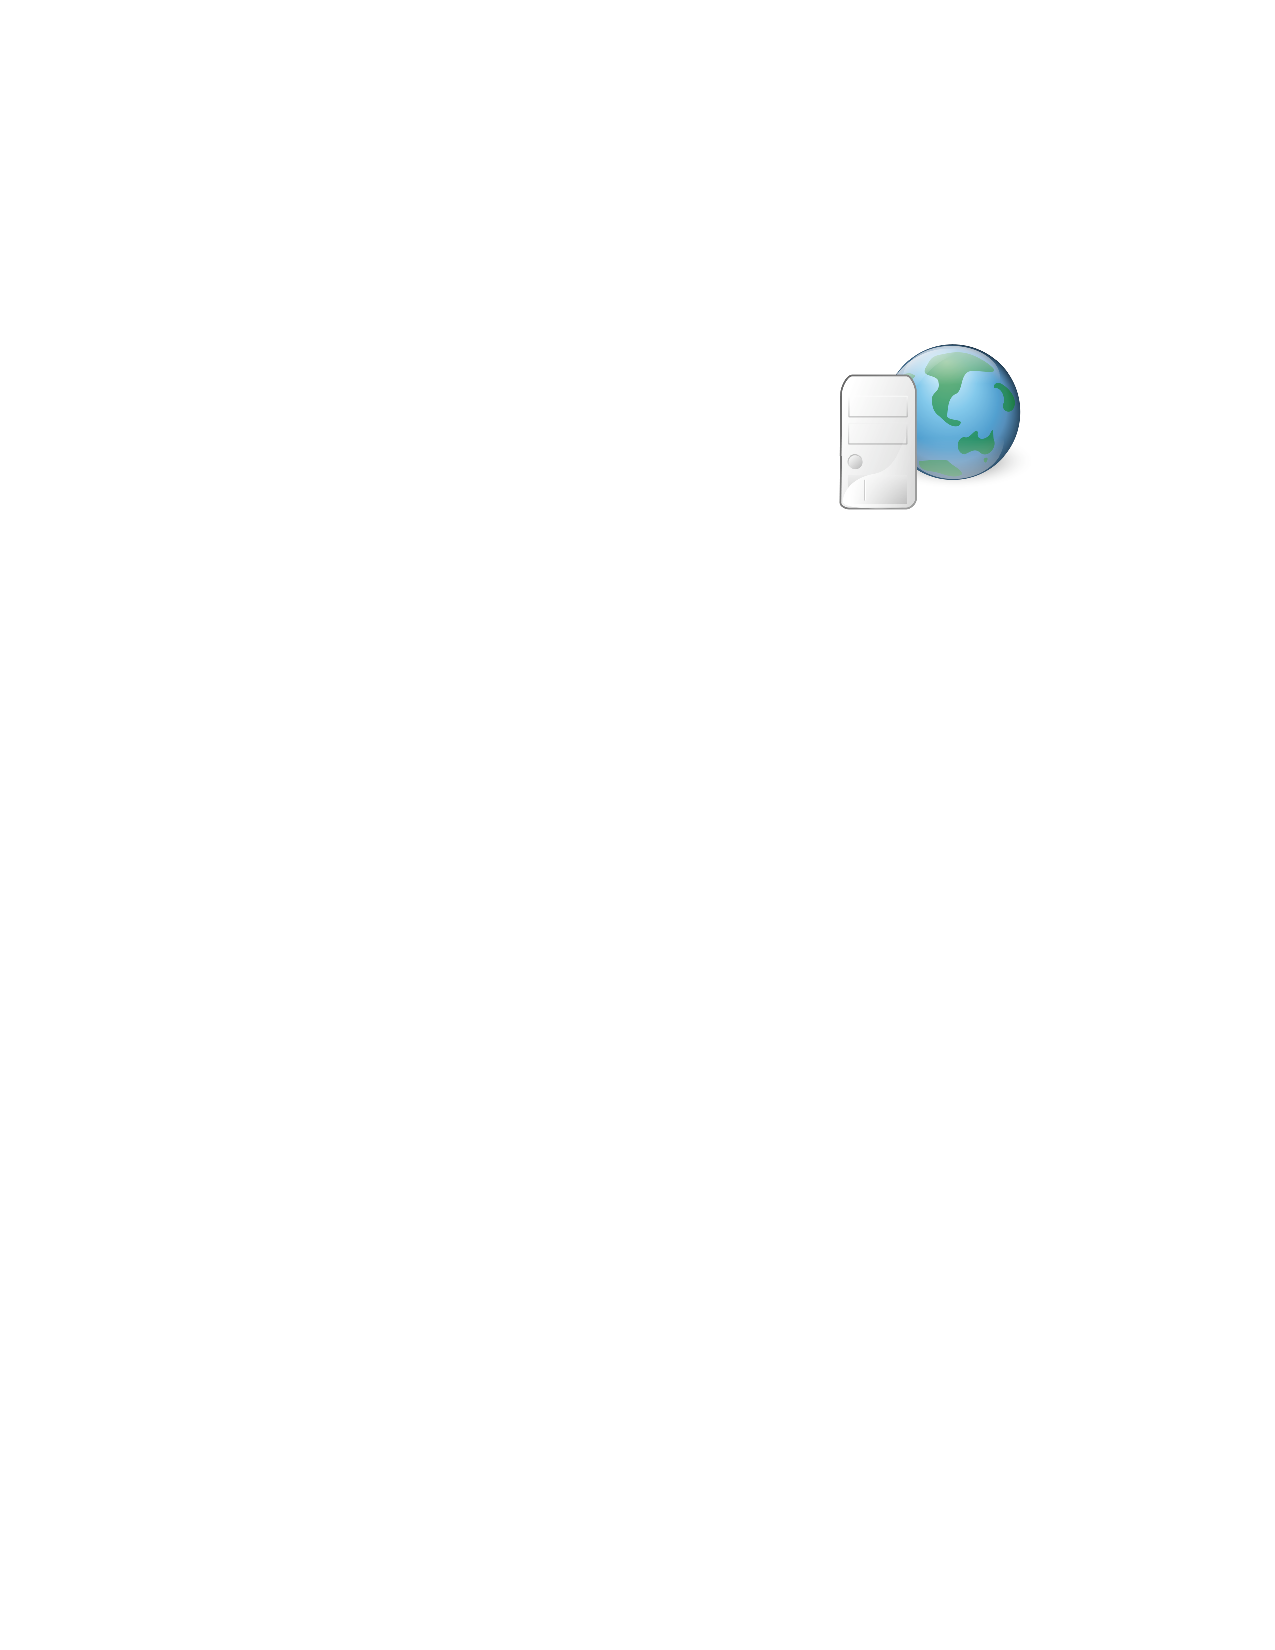
\includegraphics[width=1.5cm]{figures/webserver}};
		\node[shape=cylinder,draw=httpdcolor,thick,shape border rotate=90,xshift=1.25cm,yshift=-0.25cm,minimum width=1.2cm,fill=httpdcolor,fill opacity=0.5] at (0,0) {};
	\end{scope}
	
	\draw[httpdcolor,very thick,<-,curve to,out=180,in=0] (webserver.west) to node[fill=white,key,draw,cloud,aspect=2] {\parbox{2.5cm}{\centering HTTP Content Distribution Network}} ($(cvmfs.east)+(\gap cm,0)$);
	
	\node[key] (volimage) at (1.75cm,-2.25cm) {\parbox{3cm}{\centering File System Buffers}};
	\node[key] (volcache) at (6.25cm,-2.25cm) {\parbox{3.5cm}{\centering CernVM-FS\\ Hard Disk Cache}};
	\node[key] (volrelease) at (13.25cm,-2.25cm) {\parbox{3.5cm}{\centering CernVM-FS ``Repository''\\ (All Releases Available)}};
	\draw[decorate,decoration={expanding waves,segment length=0.1cm,angle=7}] (volimage.east) -- (volcache.west);
	\draw[decorate,decoration={expanding waves,segment length=0.1cm,angle=7}] (volcache.east) -- (volrelease.west);
	
\end{tikzpicture}

%\end{document}
}
	\end{center}
	\caption{Building blocks of \cernvm\ 2. \cernvm\ is built around a minimal SL5. Experiment software is loaded file by file on demand and is locally cached.}
	\label{fig:concept}
\end{figure}

\begin{figure}
	\begin{center}
		%\documentclass[a4paper, 11pt]{article}\usepackage{tikz,ifthen}\usetikzlibrary{arrows,positioning,shapes,topaths,calc,fit,backgrounds,matrix,shadows}\begin{document}

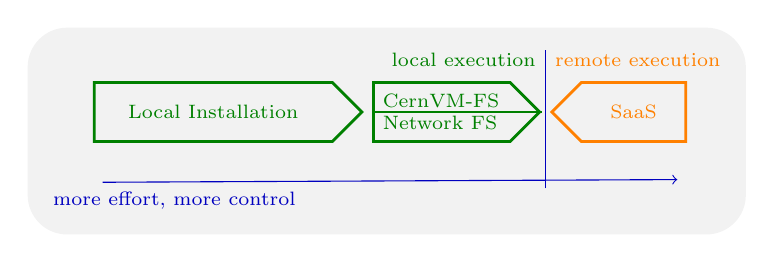
\begin{tikzpicture}
	[cell/.style={node distance=3pt,draw,minimum height=0.75cm,font=\scriptsize,line width=1pt},
	background/.style={
		rectangle,
		fill=gray!10,
		inner sep=0.2cm,
		rounded corners=5mm}
	]
		
	\node[cell,signal,signal to=east,green!50!black,minimum width=3.4cm] (AutoUpd) at (0,0) {Local Installation};
	\node[cell,signal,signal to=east,green!50!black,minimum width=1.7cm] (cvmfs) [right = of AutoUpd] {\parbox{1.5cm}{CernVM-FS\\Network FS}};
	\draw[green!50!black,line width=1pt] (cvmfs.west) -- (cvmfs.east);
	\node[cell,signal,signal to=west,orange,minimum width=1.7cm] (SaaS) [right = of cvmfs] {SaaS};
	\node[yshift=-0.5cm] (scaleleft) at (AutoUpd.south west) {};
	\node[yshift=-0.5cm] (scaleright) at (SaaS.south east) {};
	\draw[->,blue!75!black] (scaleleft) -- node[below, very near start] (morecontrol) {\scriptsize more effort, more control} (scaleright);
	\node[xshift=-0.45cm,yshift=1.3cm] (scaletop) at (SaaS.south west) {};
	\node[xshift=-0.45cm,yshift=-0.7cm] (scalebottom) at (SaaS.south west) {};
	\draw[blue!75!black] (scalebottom) -- node[yshift=0.1cm,left,very near end,green!50!black] {\scriptsize local execution}
								       node[yshift=0.1cm,right,very near end,orange] (remote){\scriptsize remote execution} (scaletop);
					       
	\begin{pgfonlayer}{background}
		\node[background,fit=(morecontrol) (remote)] (bg) {};
		%\node[anchor=north west,green!50!black] at (bg.north west) {\emph{classification}};
	\end{pgfonlayer}
\end{tikzpicture}

%\end{document}
	\end{center}
	\caption{Classification of \cvmfs\ and several alternative options for software installation.}
	\label{fig:classification}
\end{figure}

\begin{figure}
	\begin{center}
		%\documentclass[a4paper, 11pt]{article}\usepackage{tikz,ifthen}\usetikzlibrary{arrows,positioning,shapes,topaths,calc,fit,backgrounds,matrix,shadows}\begin{document}

\begin{tikzpicture}
	[block/.style={node distance=0.5cm,draw,minimum height=0.7cm,font=\footnotesize,minimum width=3cm},
	 fig/.style={}]
	 
	 \colorlet{cvmfscolor}{green!50!black}
	
	\node[block] (open) at (0,0) {\texttt{open(/ChangeLog)}};
	\node[block] (glibc) [below = of open] {glibc};
	
	\node[block, minimum height=2.5cm,yshift=-1cm] (vfs) [below = of glibc] {\parbox{2.5cm}{\centering VFS\\inode cache\\dentry cache}};
	\node[block, minimum height=1cm,yshift=0.25cm] (buffer cache) [below = of vfs] {\parbox{2.5cm}{\centering Buffer cache}};
	\node[block] (ext3) [right = of buffer cache.south east,yshift=0.35cm,xshift=0.5cm] {ext3};
	\node[block] (NFS) [above = of ext3] {NFS};
	\node (dots) [node distance=0,above = of NFS,yshift=0.3cm] {$\vdots$};
	\node[block] (Fuse) [above = of NFS,yshift=0.6cm] {Fuse};
	\node (vfsv) [left = of Fuse] {};
	
	\node[block] (libfuse) [right = of glibc, xshift=0.5cm] {libfuse};
	\node[block, cvmfscolor, very thick] (cvmfs) [above = of libfuse] {CernVM-FS};
	
	\node[fig] (sqlite) [right = of cvmfs,xshift=1cm,yshift=-1.25cm] {\includegraphics[width=1cm]{figures/memcache} 
\includegraphics[width=2.5cm]{figures/sqlite}};
	\node[fig] (cache) [right = of cvmfs,xshift=1cm,yshift=0.5cm] {
\includegraphics[width=1cm]{figures/cache}};
	\node[fig] (webserver) [right = of cache,yshift=1.5cm] {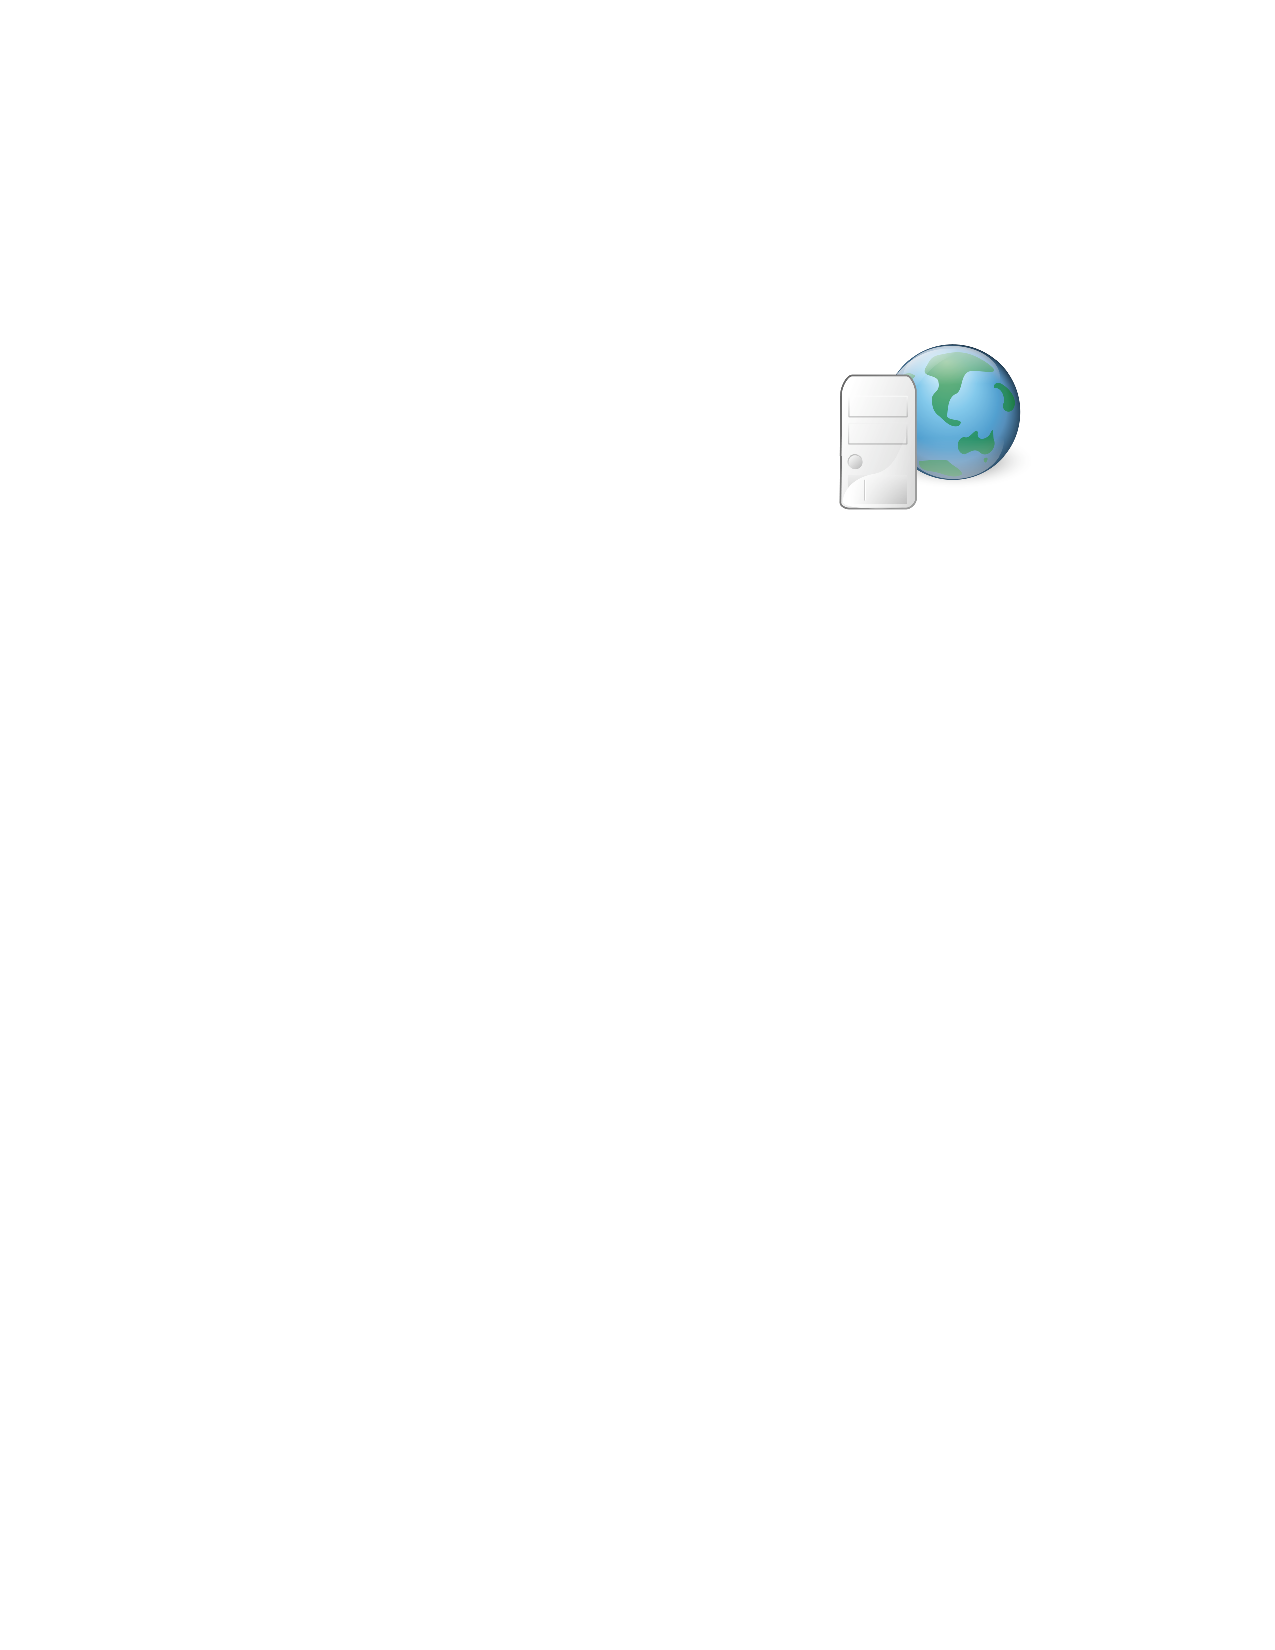
\includegraphics[width=2cm]{figures/webserver}};
	
	\node[node distance=0.8cm] (splitleft) [below=of glibc,xshift=-2cm] {};
	\node[node distance=0.8cm] (splitright) [below=of glibc,xshift=+12cm] {};
	\draw[dashed,blue] (splitleft) -- node[blue,above,very near end,anchor=south west] {\footnotesize user space} node[blue,below,very near end,anchor=north west] {\footnotesize kernel space} (splitright);
	
	\draw[->] (open) -- (glibc);
	\draw[->] (glibc) -- node[fill=white,yshift=-1ex] {\footnotesize  syscall} (vfs);
	\draw[->] (vfsv) -- (Fuse);
	\draw[->] (Fuse) -- node[fill=white,yshift=-1ex] {\footnotesize\tt  /dev/fuse} (libfuse);
	\draw[->] (libfuse) -- (cvmfs);
	
	%\draw[->,curve to,out=300,in=200] (cvmfs.south east) to node {} (sqlite.south west) {};
	\draw[->,very thick,cvmfscolor,curve to,out=180,in=10] (sqlite.west) to node [fill=white] {\footnotesize SHA1} (cvmfs.south east) {};
	\draw[<-,very thick,cvmfscolor] (cvmfs.east) -- node[fill=white] {\footnotesize file descr.} (cache.west) {};
	\draw[->, dashed] (cvmfs.west) -- node[above] {\footnotesize fd} (open.east) {};
	\draw[->,very thick,orange,curve to,out=-40,in=-140] (cache.east) to node [near start, right=0.01cm, fill=white] {\footnotesize HTTP GET} (webserver.south west) {};
	\draw[->,very thick,orange,curve to,out=160,in=40] (webserver.west) to node [near start, left=0.01cm, fill=white] {\footnotesize inflate+verify} (cache.north east) {};

	%\draw[<->, dashed, gray, curve to, out=-45,in=20] (cache.south east) to node {} (ext3.east) {};
	
\end{tikzpicture} 

%\end{document}

	\end{center}
	\caption{Process of opening a file. \cvmfs\ resolves the name by means of an SQLite catalog, which is prepended by a memory cache. Downloaded files are verified against the cryptographic hash of the corresponding catalog entry. The \texttt{read()} and the \texttt{stat()} system call can be entirely served from the in-kernel file system buffers.}
	\label{fig:fuse}
\end{figure}


\chapter{Getting Started}
\label{sct:start}

This section describes how to install the \cvmfs\ client.
\cvmfs\ is supported on Scientific Linux 5 and 6, Ubuntu 12.04, openSuSE 12.2, Fedora 17, and Mac OS X.

\section{Getting the Software}
The \cvmfs\ source code and binary packages are available under \url{https://cernvm.cern.ch/portal/downloads}.
Binary packages are produced for \rpm, \dpkg, and Mac OS X (.pkg).
\yum\ repositories for \SI{64}{\bit} and \SI{32}{\bit} Scientific Linux 5 and 6 are available under \url{http://cvmrepo.web.cern.ch/cvmrepo/yum}.
The \texttt{cvmfs-release} packages can be used to add a these \yum\ repositories to the local \yum\ installation.
The \texttt{cvmfs-release} packages are available under \url{https://cernvm.cern.ch/portal/downloads}.

The \cvmfs\ client is not relocatable and needs to be installed under /usr.
In order to compile and install from sources, use the following \cmake\ command:
\begin{verbatim}
  cmake .
  make
  sudo make install
\end{verbatim}

\section{Installation}
\subsection{Linux}
To install, proceed according to the following steps:
\begin{description}
	\item[Step 1] Install the \cvmfs\ packages.  With yum, run
\begin{verbatim}
  yum install cvmfs-keys cvmfs cvmfs-init-scripts.
\end{verbatim}
			      If yum does not show the latest packages, clean the yum cache by \texttt{yum clean all}.
			      Use \texttt{rpm -vi} to install the packages using just \rpm.
			      On Ubuntu, use \texttt{dpkg -i} on the cvmfs .deb package.
    \item[Step 2] For the base setup, run \texttt{cvmfs\_config setup}.
    				Alternatively, you can do the base setup by hand: ensure that \texttt{user\_allow\_other} is set in /etc/fuse.conf and ensure that \texttt{/cvmfs /etc/auto.cvmfs} is set in /etc/auto.master.
					If you migrate from a previous version of \cvmfs, check the release notes if there is anything special to do for migration.
	\item[Step 3] Create /etc/cvmfs/default.local and open the file for editing.
	\item[Step 4] Select the desired repositories by setting \texttt{CVMFS\_REPOSITORIES=repo1,repo2,...}.
		For ATLAS, for instance, set 
\begin{verbatim}
  CVMFS_REPOSITORIES=atlas.cern.ch,atlas-condb.cern.ch,grid.cern.ch
\end{verbatim}
		Specify the HTTP proxy servers on your site with
\begin{verbatim}
  CVMFS_HTTP_PROXY="http://myproxy1:port|http://myproxy2:port"
\end{verbatim}
		For the syntax of more complex HTTP proxy settings, see Section~\ref{sct:config:network}.
		Make sure your local Squid servers allow access to all the Stratum 1 web servers~\ref{sct:squid}.
		For Cern repositories, the Stratum 1 web servers are listed in /etc/cvmfs/domain.d/cern.ch.conf.
	\item[Step 5] Check if \cvmfs\ mounts the specified repositories by \texttt{cvmfs\_config probe}.
\end{description}

\subsection{Mac OS X}
On Mac OS X, \cvmfs\ is based on \fusex\footnote{\url{http://fuse4x.github.com}}. 
It is not yet integrated with \autofs.
In order to install, proceed according to the following steps:
\begin{description}
	\item[Step 1] Install the \cvmfs\ package by opening the .pkg file.
	\item[Step 2] Create /etc/cvmfs/default.local and open the file for editing.
	\item[Step 3] Select the desired repositories by setting \texttt{CVMFS\_REPOSITORIES=repo1,repo2,...}.
		For CMS, for instance, set 
\begin{verbatim}
  CVMFS_REPOSITORIES=cms.cern.ch
\end{verbatim}
		Specify the HTTP proxy servers on your site with
\begin{verbatim}
  CVMFS_HTTP_PROXY="http://myproxy1:port|http://myproxy2:port"
\end{verbatim}
	If you're unsure about the proxy names, set \texttt{CVMFS\_HTTP\_PROXY=DIRECT}.
    \item[Step 4] Mount your repositories like
\begin{verbatim} 
  sudo mkdir -p /cvmfs/cms.cern.ch
  sudo mount -t cvmfs cms.cern.ch /cvmfs/cms.cern.ch
\end{verbatim}
\end{description}

\section{Usage}
The \cvmfs\ repositories are located under /cvmfs.
Each repository is identified by a \emph{fully qualified repository name}.
The fully qualified repository name consists of a repository identifier and a domain name, similar to DNS records~\cite{rfc1035}.
The domain part of the fully qualified repository name indicates the location of repository creation and maintenance.
For the ATLAS experiment software, for instance, the fully qualified repository name is atlas.cern.ch although the hosting web servers are spread around the world.

Mounting and un-mounting of the \cvmfs\ is controlled by \autofs\ and \product{automount}.
That is, starting from the base directory /cvmfs different repositories are mounted automatically just by accessing them.
For instance, running the command \texttt{ls /cvmfs/atlas.cern.ch} will mount the ATLAS software repository.
This directory gets automatically unmounted after some \product{automount}-defined idle time.

\section{Debugging Hints}
\label{sct:debugginghints}

In order to check for common misconfigurations in the base setup, run
\begin{verbatim}
  cvmfs_config chksetup
\end{verbatim}

\cvmfs\ gathers its configuration parameter from various configuration files that can overwrite each others settings (default configuration, domain specific configuration, local setup, \dots).  
To show the effective configuration for \emph{repository}.cern.ch, run
\begin{verbatim}
  cvmfs_config showconfig repository.cern.ch
\end{verbatim}

In order to exclude \product{autofs}/\product{automounter} as a source of problems, you can try to mount \emph{repository}.cern.ch manually by
\begin{verbatim}
  mkdir -p /mnt/cvmfs
  mount -t cvmfs repository.cern.ch /mnt/cvmfs
\end{verbatim}

In order to exclude SELinux as a source of problems, you can try mounting after SELinux has been disabled by
\begin{verbatim}
  /usr/sbin/setenforce 0
\end{verbatim}

Once you sorted out a problem, make sure that you do not get the original error served from the file system buffers by
\begin{verbatim}
  service autofs restart
\end{verbatim}

In case you need additional assistance, please don't hesitate to contact us at \url{cernvm.support@cern.ch}.
Together with the problem description, please send the system information tarball created by \texttt{cvmfs\_config bugreport}.


\chapter{Client Configuration}

\section{Structure of /etc/cvmfs}
The local configuration of \cvmfs\ is controlled by several files in \texttt{/etc/cvmfs} listed in Table~\ref{tbl:configfiles}.
For every .conf file except for site.conf you can create a corresponding .local file having the same prefix in order to customize the configuration.
The .local file will be sourced after the corresponding .conf file.

In a typical installation, a handful of parameters need to be set in /etc/cvmfs/default.local.
Most likely, this is the list of repositories (\texttt{CVMFS\_REPOSITORIES}), HTTP proxies (see Section~\ref{sct:config:network}), and perhaps the cache directory and the cache quota (see Section~\ref{sct:config:cache})
In a few cases, one might change a parameter for a specific domain or a specific repository, \eg provide an exclusive cache for a specific repository (see Section~\ref{sct:config:cache}).

The .conf and .local configuration files are key-value pairs in the form \texttt{PARAMETER=value}.
They are sourced by /bin/sh.
Hence, a limited set of shell commands can be used inside these files including comments, \texttt{if} clauses, parameter evaluation, and shell math (\texttt{\$((\dots))}).
Special characters have to be quoted.
For instance, instead of \texttt{CVMFS\_HTTP\_PROXY=p1;p2}, write \texttt{CVMFS\_HTTP\_PROXY='p1;p2'} in order to avoid parsing errors.
For a list of all parameters, see Appendix~\ref{apx:parameters}.

\begin{table}
	\begin{center}
		\begin{tabularx}{\linewidth}{lX}
			\toprule
			{\bf\centering File} & {\bf\centering Purpose} \\
			\midrule
			\texttt{config.sh} & Set of internal helper functions \\
			\texttt{default.conf} & Set of parameters reflecting the standard configuration \\
			\texttt{site.conf} & Site specific set of parameters that overwrites the standard configuration.  
				This file is used by the \cernvm\ contextualization. \\
			\texttt{domain.d/\$domain.conf} & Domain-specific parameters and implementations of the functions in \texttt{config.sh} \\
			\texttt{config.d/\$repository.conf} & Repository-specific parameters and implementations of the functions in \texttt{config.sh} \\
			\texttt{keys/*.pub} & Public keys used to verify the digital signature of file catalogs \\
			\bottomrule
		\end{tabularx}
	\end{center}
	\caption{List of configuration files for \cvmfs\ in \texttt{/etc/cvmfs}}
	\label{tbl:configfiles}
\end{table}


\section{Mounting}
Typically, mounting of \cvmfs\ repositories is handled by \autofs.
Just by accessing a repository directory under /cvmfs (\eg /cvmfs/atlas.cern.ch), \autofs\ will take care of mounting.
\autofs\ will also automatically unmount a repository if it is not used for a while.

Instead of using \autofs, \cvmfs\ repositories can be mounted manually with the system's \texttt{mount} command.
In order to do so, use the \texttt{cvmfs} file system type, like
\begin{verbatim}
  mount -t cvmfs atlas /cvmfs/atlas.cern.ch
\end{verbatim}
Likewise, \cvmfs\ repositories can be mounted through entries in /etc/fstab.
A sample entry in /etc/fstab:
\begin{verbatim}
  atlas.cern.ch /mnt/test cvmfs defaults 0 0
\end{verbatim}

Every mount point corresponds to a \cvmfs\ process.
Using \autofs\ or the system's mount command, every repository can only be mounted once.
Otherwise multiple \cvmfs\ processes would collide in the same cache location.
If a repository is needed under several paths, use a \emph{bind mount} or use a private file system mount point (see Section~\ref{sct:privatemount}).

\subsection{Private Mount Points}
\label{sct:privatemount}
In contrast to the system's \texttt{mount} command which requires root privileges, \cvmfs\ can also be mounted like other Fuse file systems by normal users.
In this case, \cvmfs\ uses parameters from one or several user-provided config files instead of using the files under /etc/cvmfs.
\cvmfs\ private mount points do not appear as \texttt{cvmfs2} file systems but as \texttt{fuse} file systems.
The \texttt{cvmfs\_config} and \texttt{cvmfs\_talk} commands do not affect privately mounted \cvmfs\ repositories.
On an interactive machine, private mount points are for instance unaffected by an administrator unmounting all system's \cvmfs\ mount points by \texttt{cvmfs\_config unmount}.

In order to mount \cvmfs\ privately, use the \texttt{cvmfs2} command like
\begin{verbatim}
  cvmfs2 -o config=myparams.conf atlas.cern.ch /home/user/myatlas
\end{verbatim}
A minimal sample myparams.conf file could look like this:
\begin{verbatim}
  CVMFS_CACHE_BASE=/home/user/mycache
  CVMFS_RELOAD_SOCKETS=/home/user/mycache
  CVMFS_SERVER_URL=http://cvmfs-stratum-one.cern.ch/opt/atlas
  CVMFS_HTTP_PROXY=DIRECT
\end{verbatim}

Make sure to use absolute path names for the mount point and for the cache directory.
Use \texttt{fusermount -u} in order to unmount a privately mounted \cvmfs\ repository.

The private mount points can also be used to use the \cvmfs\ Fuse module where it has not been installed under /usr and /etc.
If the public keys are not installed under /etc/cvmfs/keys, the directory of the keys needs to be specified in the config file by \texttt{CVMFS\_KEYS\_DIR=<directory>}.
If the libcvmfs\_fuse.so library is not installed in one of the standard search paths, the \texttt{LD\_LIBRARY\_PATH} variable has to be set accordingly for the \texttt{cvmfs2} command.

\section{Network Settings}
\label{sct:config:network}
\cvmfs\ uses HTTP~\cite{rfc1945,rfc2616} for data transfer.
Repository data can be replicated to multiple web servers and cached by standard web proxies such as Squid.
In a typical setup, repositories are replicated to a handful of web servers in different locations.
These replicas form the \cvmfs\ Stratum 1 service, whereas the replication source server is the \cvmfs\ Stratum 0 server.
On every cluster of machines, there should be two or more web proxy servers that \cvmfs\ can use (see Section~\ref{sct:squid}).
These site-local web proxies reduce the network latency for the \cvmfs\ clients and they reduce the load for the Stratum 1 service.
\cvmfs\ supports choosing a random proxy for load-balancing and automatic fail-over to other hosts and proxies in case of network errors.
Roaming clients can connect directly to the Stratum 1 service.

\subsection{Stratum 1 List}
To specify the Stratum 1 servers, set \texttt{CVMFS\_SERVER\_URL} to a semicolon-separated list of known replica servers (enclose in quotes). 
The so defined URLs are organized as a ring buffer.
Whenever download of files fails from a server, \cvmfs\ automatically switches to the next mirror server.
For repositories under the cern.ch domain, the Stratum 1 servers are specified in /etc/cvmfs/domain.d/cern.ch.conf.

It is recommended to adjust the order of Stratum 1 server so that the closest servers are used with priority.
For roaming clients (\ie clients not using a proxy server), the Stratum 1 servers can be automatically sorted according to round trip time by \texttt{cvmfs\_talk host probe} (see Section~\ref{sct:tools}).
Otherwise, the proxy server would invalidate round trip time measurement.

The special sequence \texttt{@org@} in the \texttt{CVMFS\_SERVER\_URL} string is replaced by the repository name (not fully qualified).
That allows to use the same parameter for many repositories hosted under the same domain.
For instance, \texttt{http://cvmfs-stratum-one.cern.ch/opt/@org@} can resolve to \url{http://cvmfs-stratum-one.cern.ch/opt/atlas}, \url{http://cvmfs-stratum-one.cern.ch/opt/cms}, and so on depending on the repository that is being mounted.
The same works for the sequence \texttt{@fqrn@} with fully qualified repository names (\eg atlas.cern.cn, cms.cern.ch, \dots).

\subsection{Proxy Lists}
\cvmfs\ uses a dedicated HTTP proxy configuration, independent from system-wide settings. 
Instead of a single proxy, \cvmfs\ uses a \emph{chain of load-balanced proxy groups}.
The \cvmfs\ proxies are set by the \texttt{CVMFS\_HTTP\_PROXY} parameter.

Proxies within the same proxy group are considered as a load-balance group and a proxy is selected randomly.
If a proxy fails, \cvmfs\ automatically switches to another proxy from the current group.
If all proxies from a group have failed, \cvmfs\ switches to the next proxy group.
After probing the last proxy group in the chain, the first proxy is probed again.
To avoid endless loops, for each file download the number of switches is restricted by the total number of proxies.

The chain of proxy groups is specified by a string of semicolon separated entries, each group is a list of pipe separated hostnames\footnote{The usual proxy notation rules apply, like \texttt{http://proxy1:8080|http://proxy2:8080;DIRECT}}.
The \texttt{DIRECT} keyword for a hostname avoids using proxies.
Note that the \texttt{CVMFS\_HTTP\_PROXY} parameter is necessary in order to mount.
If you don't use proxies, set the parameter to \texttt{DIRECT}.

Multiple proxy groups are often organized as a primary proxy group at the local site and backup proxy groups at remote sites.
In order to avoid \cvmfs\ being stuck with proxies at a remote site after a fail-over, \cvmfs\ will automatically retry to use proxies from the primary group after some time.
The delay for re-trying a proxies from the primary group is set in seconds by \texttt{CVMFS\_PROXY\_RESET\_AFTER}.
The distinction of primary and backup proxy groups can be turned off by setting this parameter to 0.

\subsection{Timeouts}
\cvmfs\ tries to gracefully recover from broken network links and temporarily overloaded paths.
The timeout for connection attempts and for very slow downloads can be set by \texttt{CVMFS\_TIMEOUT} and \texttt{CVMFS\_TIMEOUT\_DIRECT}.
The two timeout parameters apply to a connection with a proxy server and to a direct connection to a Stratum 1 server, respectively.
A download is considered to be ``very slow'' if the transfer rate is below 100 Bytes/second for more than the timeout interval.
A very slow download is treated like a broken connection.

On timeout errors and on connection failures (but not on name resolving failures), \cvmfs\ will retry the path using an exponential backoff.
This introduces a jitter in case there are many concurrent requests by a cluster of nodes, allowing a proxy server or web server to serve all the nodes consecutively.
\texttt{CVMFS\_MAX\_RETRIES} sets the number of retries on a given path before \cvmfs\ tries to switch to another proxy or host. 
The overall number of requests with a given proxy/host combination is \texttt{\$CVMFS\_MAX\_RETRIES}+1.
\texttt{CVMFS\_BACKOFF\_INIT} sets the maximum initial backoff in seconds.  
The actual initial backoff is picked with milliseconds precision randomly in the interval $[1, \text{\$CVMFS\_BACKOFF\_INIT}\cdot 1000]$.
With every retry, the backoff is then doubled.

\section{Cache Settings}
\label{sct:config:cache}
Downloaded files will be stored in a local cache directory.
The \cvmfs\ cache has a soft quota; as a safety margin, the partition hosting the cache should provide \SI{15}{\percent} more space than the soft quota limit.
Once the quota limit is reached, \cvmfs\ will automatically remove files from the cache according to the least recently used policy~\cite{lru06}.
Removal of files is performed bunch-wise until half of the maximum cache size has been freed.
Currently, \cvmfs\ is not able to access files in the repository that are larger than half of the cache quota.
The quota limit can be set in Megabytes by \texttt{CVMFS\_QUOTA\_LIMIT}.
For typical repositories, a few Gigabytes make a good quota limit.
For repositories hosted at \cern, quota recommendations can be found under \url{http://cernvm.cern.ch/portal/cvmfs/examples}.

The cache directory needs to be on a local file system in order to allow each host the accurate accounting of the cache contents; on a network file system, the cache can potentially be modified by other hosts.
Furthermore, the cache directory is used to create (transient) sockets and pipes, which is usually only supported by a local file system such as ext3 or XFS.
The location of the cache directory can be set by \texttt{CVMFS\_CACHE\_BASE}.

Each repository can either have an exclusive cache or join the \cvmfs\ shared cache.
The shared cache enforces a common quota for all repositories used on the host.
File duplicates across repositories are stored only once in the shared cache.
The quota limit of the shared directory should be at least the maximum of the recommended limits of its participating repositories.
In order to have a repository not join the shared cache but use an exclusive cache, set \texttt{CVMFS\_SHARED\_CACHE=no}.

\subsection{Alien Cache}
An ``alien cache'' provides the possibility to use a data cache outside the control of \cvmfs.
This can be necessary in HPC environments where local disk space is not available or scarce but powerful cluster file systems are available.
The alien cache directory is a directory in addition to the ordinary cache directory.
The ordinary cache directory is still used to store control files.

The alien cache directory is set by the \texttt{CVMFS\_ALIEN\_CACHE} option.
It can be located anywhere including cluster and network file systems
If configured, all data chunks are stored there.
\cvmfs\ ensures atomic access to the cache directory.
It is safe to have the alien directory shared by multiple \cvmfs\ processes and it is safe to unlink files from the alien cache directory anytime.
The contents of files, however, must not be touched by third-party programs.

In contrast to normal cache mode where files are store in mode 0600, in the alien cache files are stored in mode 0660.  
So all users being part of the alien cache directory's owner group can use it.

The skeleton of the alien cache directory should be created upfront.
Otherwise, the first \cvmfs\ process accessing the alien cache determines the ownership.
The \texttt{cvmfs2} binary can create such a skeleton using
\begin{verbatim}
cvmfs2 __MK_ALIEN_CACHE__ $alien_cachedir $owner_uid $owner_gid
\end{verbatim}

Since the alien cache is unmanaged, there is no automatic quota management provided by \cvmfs; the alien cache directory is ever-growing.
The \texttt{CVMFS\_ALIEN\_CACHE} requires \texttt{CVMFS\_QUOTA\_LIMIT=-1} and \texttt{CVMFS\_SHARED\_CHACE=no}.

The alien cache might be used in combination with a special repository replication mode that preloads a cache directory (\cf Section~\ref{sct:replica}).
This allows to propagate an entire repository into the cache of a cluster file system for HPC setups that do not allow outgoing connectivity.

\section{NFS Server Mode}
In case there is no local hard disk space available on a cluster of worker nodes, a single \cvmfs\ client can be exported via NFS~\cite{rfc1813,rfc3530} to these worker nodes.
This mode of deployment will inevitably introduce a performance bottleneck and a single point of failure and should be only used if necessary.

NFS export requires Linux kernel >= 2.6.27 on the NFS server.
It works for Scientific Linux 6 but not for Scientific Linux 5.
NFS clients can run both SL5 and SL6.
The NFS server should run a lock server as well.
For proper NFS support, set \texttt{CVMFS\_NFS\_SOURCE=yes}. 
Also, \autofs\ for \cvmfs\ needs to be turned off and repositories need to be mounted manually.

In the NFS mode, upon mount an additionally directory nfs\_maps.\$repository\_name appears in the \cvmfs\ cache directory.
These \emph{NFS maps} use \leveldb\ to store the virtual inode \cvmfs\ issues for any accessed path.
The virtual inode may be requested by NFS clients anytime later.
As the NFS server has no control over the lifetime of client caches, entries in the NFS maps cannot be removed.

Typically, every entry in the NFS maps requires some 150-200 Bytes. 
A recursive \texttt{find} on /cvmfs/atlas.cern.ch with 25 million entries, for instance, would add up \SI{5}{\giga\byte} in the cache directory. 
For a \cvmfs\ instance that is exported via NFS, the safety margin for the NFS maps needs be taken into account.
It also might be necessary to monitor the actual space consumption.

\subsection{Tuning}
For decent performance, the amount of memory given to the meta-data cache should be increased. 
By default, this is 16M.
It can be increased, for instance, to 256M by setting \texttt{CVMFS\_MEMCACHE\_SIZE} to 256.
Furthermore, the maximum number of download retries should be increased to at least 2 for the NFS use case.

The number of NFS daemons should be increased as well.
A value of 128 NFS daemons has shown perform well.
In Scientific Linux, the number of NFS daemons is set by the \texttt{RPCNFSDCOUNT} parameter in /etc/sysconfig/nfs.

The performance will benefit from large RAM on the NFS server ($\geq\SI{16}{\giga\byte}$) and \cvmfs\ caches hosted on an SSD hard drive.

\subsection{Shared NFS Maps (HA-NFS)}
As an alternative to the existing, \leveldb\ managed NFS maps, the NFS maps can optionally be managed out of the \cvmfs\ cache directory by \sqlite.
This allows the NFS maps to be placed on shared storage and accessed by multiple \cvmfs\ NFS export nodes simultaneously for clustering and active high-availablity setups.
In order to enable shared NFS maps, set \texttt{CVMFS\_NFS\_SHARED} to the path that should be used to host the \sqlite\ database.  
If the path is on shared storage, the shared storage has to support POSIX file locks.
The drawback of the \sqlite\ managed NFS maps is a significant performance penalty which in practice can be covered by the memory caches.

\subsection{Example}
An example entry /etc/exports (note: the fsid needs to be different for every exported \cvmfs\ repository)
\begin{verbatim}
  /cvmfs/atlas.cern.ch 172.16.192.0/24(ro,sync,no_root_squash,\
    no_subtree_check,fsid=101)
\end{verbatim}
A sample entry /etc/fstab entry on a client:
\begin{verbatim}
  172.16.192.210:/cvmfs/atlas.cern.ch /cvmfs/atlas.cern.ch nfs \
    ro,nfsvers=3,noatime,nodiratime,ac,actimeo=60,lookupcache=all 0 0
\end{verbatim}


\section{Hotpatching and Reloading}
\label{sct:hotpatch}

By hotpatching a running \cvmfs\ instance, most of the code can be reloaded without unmounting the file system.
The current active code is unloaded and the code from the currently installed binaries is reloaded.
Hotpatching is logged to syslog.
Since \cvmfs\ is re-initialized during hotpatching and configuration parameters are re-read, hotpatching can be also seen as a ``reload''.

Hotpatching has to be done for all repositories concurrently by
\begin{verbatim}
  cvmfs_config [-c] reload
\end{verbatim}
The optional parameter \texttt{-c} specifies if the \cvmfs\ cache should be wiped out during the hotpatch.
Reloading of the parameters of a specific repository can be done like
\begin{verbatim}
  cvmfs_config reload atlas.cern.ch
\end{verbatim}
In order to see the history of loaded CernVM-FS Fuse modules, run
\begin{verbatim}
  cvmfs_talk hotpatch history
\end{verbatim}
The currently loaded set of parameters can be shown by
\begin{verbatim}
  cvmfs_talk parameters
\end{verbatim}
The \cvmfs\ packages use hotpatching in order to update previous versions.


\section{Auxiliary Tools}
\label{sct:tools}

\subsection{cvmfs\_fsck}
\cvmfs\ assumes that the local cache directory is trustworthy.
However, it might happen that files get corrupted in the cache directory caused by errors outside the scope of \cvmfs.
\cvmfs\ stores files in the local disk cache with their cryptographic content hash key as name, which makes it fairly easy to verify file integrity.
\cvmfs\ contains the \texttt{cvmfs\_fsck} utility to do so for a specific cache directory. 
Its return value is comparable to the system's \texttt{fsck}.
For example,
\begin{verbatim}
  cvmfs_fsck -j 8 /var/lib/cvmfs/shared
\end{verbatim}
checks all the data files and catalogs in \texttt{/var/lib/cvmfs/shared} using 8 concurrent threads.  
Supported options are:

\begin{tabularx}{\linewidth}{lX}
	\texttt{-v}				& Produce more verbose output.\\
	\texttt{-j \#threads}	& Sets the number of concurrent threads that check files in the cache directory. Defaults to 4. \\
	\texttt{-p} 			& Tries to automatically fix problems. \\
	\texttt{-f} 			& Unlinks the cache database.  The database will be automatically rebuilt by \cvmfs\ on next mount.\\
\end{tabularx}

\subsection{cvmfs\_config}
The \texttt{cvmfs\_config} utility provides commands in order to setup the system for use with \cvmfs.
\begin{description}
	\item[setup] The \texttt{setup} command takes care of basic setup tasks, such as creating the cvmfs user and allowing access to \cvmfs\ mount points by all users.
	\item[chksetup] The \texttt{chksetup} command inspects the system and the \cvmfs\ configuration in /etc/cvmfs for common problems.
	\item [showconfig] The \texttt{showconfig} command prints the \cvmfs\ parameters for all repositories or for the specific repository given as argument.
	\item [stat] The \texttt{stat} command prints file system and network statistics for currently mounted repositories.
	\item [status] The \texttt{status} command shows all currently mounted repositories and the process id (PID) of the \cvmfs\ processes managing a mount point.
	\item [probe] The \texttt{probe} command tries to access /cvmfs/\$repository for all repositories specified in \texttt{CVMFS\_REPOSITORIES}.
	\item [reload] The \texttt{reload} command is used to reload or hotpatch \cvmfs\ instances (see Section~\ref{sct:hotpatch}).
	\item [unmount] The \texttt{unmount} command unmounts all currently mounted \cvmfs\ repositories, which will only succeed if there are no open file handles on the repositories.
	\item [wipecache] The \texttt{wipecache} command tries to unmount all currenlty mounted \cvmfs\ repositories and, in case of success, removes all files in the \cvmfs\ cache.
	\item [bugreport] The \texttt{bugreport} command creates a tarball with collected system information which helps to debug a problem (see Section~\ref{sct:debugginghints}). 
\end{description}

\subsection{cvmfs\_talk}
The \texttt{cvmfs\_talk} command provides a way to control a currently running \cvmfs\ process and to extract information about the status of the corresponding mount point.
Most of the commands are for special purposes only or covered by more convenient commands, such as \texttt{cvmfs\_config showconfig} or \texttt{cvmfs\_config stat}.
Two commands might be of particular interest though.
\begin{verbatim}
  cvmfs_talk cleanup 0
\end{verbatim}
will, without interruption of service, immediately cleanup the cache from all files that are not currently pinned in the cache.
\begin{verbatim}
  cvmfs_talk internal affairs
\end{verbatim}
prints the internal status information and performance counters.
It can be helpful for performance engineering.

\subsection{Other}
Information about the current cache usage can be gathered using the \texttt{df} utility.
For repositories created with the \cvmfs\ 2.1 toolchain, information about the overall number of file system entries in the repository as well as the number of entries covered by currently loaded meta-data can be gathered by \texttt{df -i}.

For the \nagios\footnote{\url{http://www.nagios.org}}~\cite{nagios08} monitoring system, a checker plugin is available under \url{http://cernvm.cern.ch/portal/filesystem/downloads}.

\section{Debug Logs}
The \texttt{cvmfs2} binary forks a watchdog process on start.
Using this watchdog, \cvmfs\ is able to create a stack trace in case certain signals (such as a segmentation fault) are received.
The watchdog writes the stack trace into syslog as well as into a file \texttt{stacktrace} in the cache directory.

In addition to the debugging hints in Section~\ref{sct:debugginghints}, \cvmfs\ can be started in debug mode.
In the debug mode, \cvmfs\ will log with high verbosity which makes the debug mode unsuitable for production use.
In order to turn on the debug mode, set \texttt{CVMFS\_DEBUGFILE=/tmp/cvmfs.log}.



\chapter{Setting up a Local Squid Proxy}
\label{sct:squid}

For clusters of nodes with \cvmfs\ clients, we strongly recommend to setup two or more \squid\footnote{\url{http://www.squid-cache.org}} forward proxy servers as well.
The forward proxies will reduce the latency for the local worker nodes, which is critical for cold cache performance. 
They also reduce the load on the Stratum 1 servers.

From what we have seen, a \squid\ server on commodity hardware scales well for at least a couple of hundred worker nodes.
The more RAM and hard disk you can devote for caching the better.
We have good experience with \SIrange{4}{8}{\giga\byte} of memory cache and \SIrange{50}{100}{\giga\byte} of hard disk cache.
We suggest to setup two identical \squid\ servers for reliability and load-balancing.
Assuming the two servers are A and B, set
\begin{verbatim}
  CVMFS_HTTP_PROXY="http://A:3128|http://B:3128"
\end{verbatim}

\squid\ is very powerful and has lots of configuration and tuning options.
For \cvmfs\ we require only the very basic static content caching.
If you already have a \emph{Frontier Squid}\footnote{\url{http://frontier.cern.ch}}~\cite{frontier08, frontier10} installed you can use it as well for \cvmfs.

Otherwise, cache sizes and access control needs to be configured in order to use the \squid\ server with \cvmfs.
In order to do so, browse through your /etc/squid/squid.conf and make sure the following lines appear accordingly:
\begin{verbatim}
  max_filedesc 8192
  maximum_object_size 1024 MB

  cache_mem 128 MB
  maximum_object_size_in_memory 128 KB
  # 50 GB disk cache
  cache_dir ufs /var/spool/squid 50000 16 256
\end{verbatim}

Furthermore, \squid\ needs to allow access to all Stratum 1 servers.
This is controlled through \squid\ ACLs.
For the Stratum 1 servers for the cern.ch, egi.eu, and opensciencegrid.org domains, add the following lines to you \squid\ configuration:
\begin{verbatim}
  acl cvmfs dst cvmfs-stratum-one.cern.ch
  acl cvmfs dst cernvmfs.gridpp.rl.ac.uk
  acl cvmfs dst cvmfs.racf.bnl.gov
  acl cvmfs dst cvmfs02.grid.sinica.edu.tw
  acl cvmfs dst cvmfs.fnal.gov
  acl cvmfs dst cvmfs-atlas-nightlies.cern.ch
  acl cvmfs dst cvmfs-egi.gridpp.rl.ac.uk
  acl cvmfs dst klei.nikhef.nl
  acl cvmfs dst cvmfsrepo.lcg.triumf.ca
  acl cvmfs dst cvmfsrep.grid.sinica.edu.tw
  acl cvmfs dst cvmfs-s1bnl.opensciencegrid.org
  acl cvmfs dst cvmfs-s1fnal.opensciencegrid.org
  http_access allow cvmfs
\end{verbatim}

The \squid\ configuration can be verified by \texttt{squid -k parse}.
Before the first service start, the cache space on the hard disk needs to be prepared by \texttt{squid -z}.
In order to make the increased number of file descriptors effective for Squid, execute \texttt{ulimit -n 8192} prior to starting the squid service.


\chapter{Creating a Repository (Stratum~0)}
\label{sct:createrepo}

% Introduction
% Components
% Installation / Requirements
% Cvmfs server and cvmfs swissknife

\cvmfs\ is a file system with a single source of (new) data.
This single source, the repository \emph{Stratum 0}, is maintained by a dedicated \emph{release manager machine} or \emph{installation box}.
A read-writable copy of the repository is accessible on the release manager machine.
The \cvmfs\ server tool kit is used to \emph{publish} the current state of the repository on the release manager machine.
Publishing is an atomic operation.

All data stored in \cvmfs\ have to be converted into a \cvmfs\ \emph{repository} during the process of publishing.
The \cvmfs\ repository is a form of content-addressable storage.
Conversion includes creating the file catalog(s), compressing new and updated files and calculating content hashes.
Storing the data in a content-addressable format results in automatic file de-duplication.
It furthermore simplifies data verification and it allows for file system snapshots.

In order to provide a writable \cvmfs\ repository, \cvmfs\ uses a union file system that combines a read-only \cvmfs\ mount point with a writable scratch area~\cite{unionfs04,aufs}.
Figure~\ref{fig:installwebserver} outlines the process of publishing a repository.

\pagebreak

\section{\cvmfs\ Server Quick-Start Guide}
\label{sct:quickstart}

\subsection{System Requirements}
\begin{itemize}
\item Apache HTTP server \emph{OR} S3 compatible storage service
\item AUFS union file system in the kernel
\item Officially supported platforms
\begin{itemize}
    \item Scientific Linux 5 (64 bit)
    \item Scientific Linux 6 (64 bit - with custom AUFS enabled kernel)
    \item Ubuntu 13.10 and above (64 bit - with installed AUFS kernel module)
\end{itemize}
\end{itemize}

\subsection{Installation}
\begin{enumerate}
\item Install \texttt{cvmfs} and \texttt{cvmfs-server} packages
\item Ensure enough disk space in \texttt{/var/spool/cvmfs} (\textgreater 50GiB)
\item For local storage: Ensure enough disk space in \texttt{/srv/cvmfs}
\item Create a repository with \texttt{cvmfs\_server mkfs} (See Section~\ref{sct:repocreation})
\end{enumerate}

\subsection{Content Publishing}
\begin{enumerate}
\item \texttt{cvmfs\_server transaction <repository name>}
\item Install content into \texttt{/cvmfs/<repository name>}
\item Create nested catalogs at proper locations
\begin{itemize}
    \item Create \texttt{.cvmfscatalog} files (See Section~\ref{sct:nestedcatalogs}) or
    \item Consider using a \texttt{.cvmfsdirtab} file (See Section~\ref{sct:dirtab})
\end{itemize}
\item \texttt{cvmfs\_server publish <repository name>}
\end{enumerate}

\subsection{Backup Policy}
\begin{itemize}
\item Create backups of signing key files in \texttt{/etc/cvmfs/keys}
\item Entire repository content
\begin{itemize}
   \item For local storage: \texttt{/srv/cvmfs}
   \item Stratum~1s can serve as last-ressort backup of repository content
\end{itemize}
\end{itemize}

\pagebreak

\section{Publishing a new Repository Revision}
\label{sct:repoupdate}

\begin{figure}[h]
	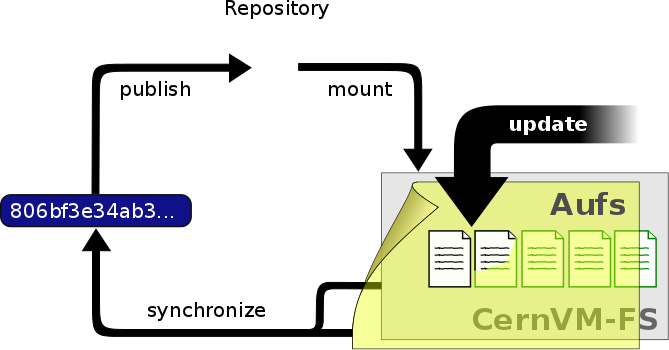
\includegraphics[width=\textwidth]{figures/update_process.png}
	\caption{Updating a mounted \cvmfs\ repository by overlaying it with a copy-on-write \aufs\ volume.
		Any changes will be accumulated in a writable volume (yellow) and can be synchronized into the \cvmfs\ repository afterwards.
		The file catalog contains the directory structure as well as file metadata, symbolic links, and secure hash keys of regular files.
		Regular files are compressed and renamed to their cryptographic content hash before copied into the data store.}
	\label{fig:installwebserver}
\end{figure}

Since the repositories may contain many file system objects\footnote{For ATLAS, for example, ``many'' means order of $10^7$ file system objects (\ie number of regular files, symbolic links, and directories).}, we cannot afford to generate an entire repository from scratch for every update.
Instead, we add a writable file system layer on top of a mounted read-only \cvmfs\ repository using the union file system \aufs~\cite{aufs}.
This renders a read-only \cvmfs\ mount point writable to the user, while all performed changes are stored in a special writable scratch area managed by \aufs.
A similar approach is used by Linux Live Distributions that are shipped on read-only media, but allow \emph{virtual} editing of files where changes are stored on a RAM disk.

If a file in the \cvmfs\ repository gets changed, \aufs\ first copies it to the writable volume and applies any changes to this copy (copy-on-write semantics).
\aufs\ will put newly created files or directories in the writable volume as well.
Additionally it creates special hidden files (called \emph{white-outs}) to keep track of file deletions in the \cvmfs\ repository.

Eventually, all changes applied to the repository are stored in \aufs's scratch area and can be merged into the actual \cvmfs\ repository by a subsequent synchronization step.
Up until the actual synchronization step takes place, no changes are applied to the \cvmfs\ repository.
Therefore, any unsuccessful updates to a repository can be rolled back by simply clearing the writable file system layer of \aufs.

\section{Requirements for a new Repository}
\label{sct:newreporequirements}

In order to create a repository, the server and client part of \cvmfs\ must be installed on the release manager machine.
Furthermore your machine should provide an \aufs\ enabled Kernel as well as a running \texttt{Apache2} web server.
Currently we support Scientific Linux 6 and Ubuntu 12.04 distributions.
Please note, that Scientific Linux 6 \emph{does not} ship with an \aufs\ enabled kernel, therefore we provide a compatible patched kernel as RPMs (see Appendix~\ref{apx:rpms}).


\pagebreak
\section{Notable \cvmfs\ Server Locations and Files}
\label{sct:repoanatomy}
There are a number of possible customisations in the \cvmfs\ server installation.
The following table provides an overview of important configuration files and intrinsical paths together with some customisation hints.
\LTXtable{\textwidth}{figures/tabserveranatomy.tex}


\section{\cvmfs\ Repository Creation and Updating}
\label{sct:repocreateandupdate}
The \cvmfs\ server tool kit provides the \texttt{cvmfs\_server} utility in order to perform all operations related to repository creation, updating, deletion, replication and inspection.
Without any parameters it prints a short documentation of its commands.

\subsection{Repository Creation}
\label{sct:repocreation}

A new repository is created by \texttt{cvmfs\_server mkfs}:
\begin{verbatim}
  cvmfs_server mkfs my.repo.name
\end{verbatim}
The utility will ask for a user that should act as the owner of the repository and afterwards create all the infrastructure for the new \cvmfs\ repository.
Additionally it will create a reasonable default configuration and generate a new release manager certificate and software signing key.
The public key in \texttt{/etc/cvmfs/keys/my.repo.name.pub} needs to be distributed to all client machines.

The \texttt{cvmfs\_server} utility will use \texttt{/srv/cvmfs} as storage location by default.
In case a separate hard disk should be used, a partition can be mounted on /src/cvmfs or /srv/cvmfs can be symlinked to another location (see Section~\ref{sct:repoanatomy}).
Besides local storage it is possible to use an S3 compatible storage service as data backend (see Section~\ref{sct:s3storagesetup}).

Once created, the repository is mounted under \texttt{/cvmfs/my.repo.name} containing only a single file called \texttt{new\_repository}.
The next steps describe how to change the repository content.

\subsubsection{Repositories for Volatile Files}
Repositories can be flagged as containing \emph{volatile} files using the \texttt{-v} option:
\begin{verbatim}
  cvmfs_server mkfs -v my.repo.name
\end{verbatim}
When \cvmfs\ clients perform a cache cleanup, they treat files from volatile repositories with priority.
Such volatile repositories can be useful, for instance, for experiment conditions data.

\subsubsection{S3 Compatible Storage Systems}
\label{sct:s3storagesetup}

\cvmfs\ can store files directly to S3 compatible storage systems, such as \product{Amazon S3}, \product{Huawei UDS} and \product{OpenStack SWIFT}.
The S3 storage settings are given as parameters to \texttt{cvmfs\_server mkfs}:
\begin{verbatim}
  cvmfs_server mkfs -s /etc/cvmfs/.../mys3.conf \
    -w http://s3.amazonaws.com/mybucket my.repo.name
\end{verbatim}

The file ``mys3.conf'' contains the S3 settings (see Table~\ref{tbl:s3confparameters}).
The ``-w'' option is used define the S3 server URL, e.g. http://localhost:3128, which is used for accessing the repository's backend storage on S3.
Note that this URL can be different than the S3 server address that is used for uploads, e.g. if a proxy server is deployed in front of the server.
Note that the buckets need to exist before the repository is created.
In the example above, a single bucket \texttt{mybucket-1-1} needs to be created beforehand.

\LTXtable{\textwidth}{figures/tabs3confparameters.tex}

In addition, if the S3 backend is configured to use multiple accounts or buckets, a proxy server is needed to map HTTP requests to correct buckets.
This mapping is needed because \cvmfs\ does not support buckets but assumes that all files are stored in a flat namespace.
The recommendation is to use a \squid\ proxy server (version $\geq 3.1.10$).
The squid.conf can look like this:
\begin{verbatim}
http_access allow all
http_port 127.0.0.1:3128 intercept
cache_peer swift.cern.ch parent 80 0 no-query originserver
url_rewrite_program /usr/bin/s3_squid_rewrite.py
cache deny all
\end{verbatim}

The bucket mapping logic is implemented in s3\_squid\_rewrite.py file.
This python script needs to read requests from stdin and write mapped URLs to stdout, for instance:
\begin{verbatim}
in: http://localhost:3128/data/.cvmfswhitelist
out: http://swift.cern.ch/cernbucket-9-91/data/.cvmfswhitelist
\end{verbatim}

\subsection{Repository Update}
\label{sct:repoupdateprocedure}
Typically a repository publisher does the following steps in order to create a new revision of a repository:
\begin{enumerate}
	\item Run \texttt{cvmfs\_server transaction} to switch to a copy-on-write enabled \cvmfs\ volume
	\item Make the necessary changes to the repository, \eg add new directories, patch certain binaries, \dots
	\item Test the software installation
	\item Do one of the following:
	\begin{itemize}
		\item Run \texttt{cvmfs\_server publish} to finalize the new repository revision \emph{or}
		\item Run \texttt{cvmfs\_server abort} to clear all changes and start over again
	\end{itemize}
\end{enumerate}

\cvmfs\ supports having more than one repository on a single server machine.
In case of a multi-repository host, the target repository of a command needs to be given as a parameter when running the \texttt{cvmfs\_server} utility.
The \texttt{cvmfs\_server resign} command should run every 30 days to update the signatures of the repository.
Most \texttt{cvmfs\_server} commands allow for wildcards to do manipulations on more than one repository at once, \eg \texttt{cvmfs\_server migrate *.cern.ch} would migrate all present repositories ending with \texttt{.cern.ch}.

\subsection{Repository Import}
The \cvmfs\ 2.1 server tools support the import of a \cvmfs\ file storage together with its corresponding signing keychain.
With \texttt{cvmfs\_server import} both \cvmfs\ 2.0 and 2.1 compliant repository file storages can be imported.

\texttt{cvmfs\_server import} works similar to \texttt{cvmfs\_server mkfs} (see \ref{sct:repocreation}) except it uses the provided data storage instead of creating a fresh (and empty) storage.
In case of a \cvmfs\ 2.0 file storage \texttt{cvmfs\_server import} also takes care of the file catalog migration into the \cvmfs\ 2.1 schema.

\subsubsection{Legacy Repository Import}
We strongly recommend to install \cvmfs\ 2.1 on a fresh or at least a properly cleaned  machine without any traces of the \cvmfs\ 2.0 installation before installing \cvmfs\ 2.1 server tools.

The command \texttt{cvmfs\_server import} requires the full \cvmfs\ 2.0 data storage which is located at /srv/cvmfs by default as well as the repository's signing keys.
Since the \cvmfs\ 2.1 server backend supports multiple repositories in contrast to its 2.0 counterpart, we recommend to move the repository's data storage to /srv/cvmfs/<FQRN> upfront to avoid later inconsistencies.

The following steps describe the transformation of a repository from \cvmfs\ 2.0 into 2.1. As an example we are using a repository called \textbf{legacy.cern.ch}.
\begin{enumerate}
	\item Make sure that you have backups of both the repository's backend storage and its signing keys
	\item Install and test the \cvmfs\ 2.1 server tools on the machine that is going to be used as new Stratum 0 maintenance machine
	\item Place the repository's backend storage data in /srv/cvmfs/\textit{legacy.cern.ch} \\ (default storage location)
	\item Transfer the repository's signing keychain to the machine (f.e. to \textapprox/legacy\_keys/)
	\item Run \texttt{cvmfs\_server import} like this:
\begin{verbatim}
    cvmfs_server import
      -o <username of repo maintainer> \
      -k ~/legacy_keys \
      -l               \ # for 2.0.x file catalog migration
      -s               \ # for further repository statistics
      legacy.cern.ch
\end{verbatim}
    \item Check the imported repository with \texttt{cvmfs\_server check legacy.cern.ch} for integrity (see \ref{sct:checkintegrity})
\end{enumerate}


\subsection{Customizable Actions Using Server Hooks}
\label{sct:serverhooks}
The \texttt{cvmfs\_server} utility allows release managers to trigger custom actions before and after crucial repository manipulation steps. This can be useful for example for logging purposes, establishing backend storage connections automatically or other workflow triggers, depending on the application.

There are six designated server hooks that are potentially invoked during the repository update procedure described in Section \ref{sct:repoupdateprocedure}:
\begin{itemize}
	\item When running \texttt{cvmfs\_server transaction}:
	\begin{itemize}
		\item \emph{before} the given repository is transitioned into transaction mode
		\item \emph{after} the transition was successful
	\end{itemize}
	\item When running \texttt{cvmfs\_server publish}:
	\begin{itemize}
		\item \emph{before} the publish procedure for the given repository is started
		\item \emph{after} it was published and remounted successfully
	\end{itemize}
	\item When running \texttt{cvmfs\_server abort}:
	\begin{itemize}
		\item \emph{before} the unpublished changes will be erased for the given repository
		\item \emph{after} the repository was successfully reverted to the last published state
	\end{itemize}
\end{itemize}
All server hooks must be defined in a single shell script file called:
\begin{verbatim}
/etc/cvmfs/cvmfs_server_hooks.sh
\end{verbatim}
The \texttt{cvmfs\_server} utility will check the existence of this script and source it.
To subscribe to the described hooks one needs to define one or more of the following shell script functions:
\begin{itemize}
	\setlength{\itemsep}{1pt}
	\item \texttt{transaction\_before\_hook()}
	\item \texttt{transaction\_after\_hook()}
\end{itemize}
\begin{itemize}
	\item \texttt{publish\_before\_hook()}
	\item \texttt{publish\_after\_hook()}
\end{itemize}
\begin{itemize}
	\item \texttt{abort\_before\_hook()}
	\item \texttt{abort\_after\_hook()}
\end{itemize}
The defined functions get called at the specified positions in the repository update process and are provided with the fully qualified repository name as their only parameter~(\texttt{\$1}).
Undefined functions automatically default to a NO-OP.
An example script is located at \texttt{cvmfs/cvmfs\_server\_hooks.sh.demo} in the \cvmfs\ sources.


\section{Maintaining a CernVM-FS Repository}

\cvmfs\ is a versioning, snapshot-based file system.
Similar to versioning systems, changes to /cvmfs/\dots are temporary until they are committed (\texttt{cvmfs\_server publish}) or discarded (\texttt{cvmfs\_server abort}).
That allows you to test and verify changes, for instance to test a newly installed release before publishing it to clients.
Whenever changes are published (committed), a new file system snapshot of the current state is created.
These file system snapshots can be tagged with a name, which makes them \emph{named snapshots}.
A named snapshot is meant to stay in the file system.
One can rollback to named snapshots and it is possible, on the client side, to mount any of the named snapshots in lieu of the newest available snapshot.

Two named snapshots are managed automatically by \cvmfs, \texttt{trunk} and \texttt{trunk-previous}.
This allows for easy unpublishing of a mistake, by rolling back to the \texttt{trunk-previous} tag.

\subsection{Integrity Check}
\label{sct:checkintegrity}
\cvmfs\ provides an integrity checker for repositories.
It is invoked by
\begin{verbatim}
cvmfs_server check
\end{verbatim}

The integrity checker verifies the sanity of file catalogs and verifies that referenced data chunks are present.
Ideally, the integrity checker is used after every publish operation.
Where this is not affordable due to the size of the repositories, the integrity checker should run regularly.

Optionally \texttt{cvmfs\_server check} can also verify the data integrity (command line flag \texttt{-i}) of each data object in the repository.
This is a time consuming process and we recommend it only for diagnostic purposes.


\subsection{Named Snapshots}
\label{sct:namedsnapshots}

Named snapshots or \emph{tags} are an easy way to organise checkpoints in the file system history.
\cvmfs\ clients can explicitly mount a repository at a specific named snapshot to expose the file system content published with this tag.
It also allows for rollbacks to previously created and tagged file system revisions.
Tag names need to be unique for each repository and are not allowed to contain spaces or spacial characters.
Besides the actual tag's name they can also contain a free descriptive text and store a creation timestamp.

Named snapshots are best to use for larger modifications to the repository, for instance when a new major software release is installed.
Named snapshots provide the ability to easily undo modifications and to preserve the state of the file system for the future.
Nevertheless, named snapshots should not be used excessively.
Less than 50 named snapshots are a good number of named snapshots in many cases.

By default, new repositories will automatically create a generic tag if no explicit tag is given during publish.
The automatic tagging can be turned off using the -g option during repository creation or by setting \texttt{CVMFS\_AUTO\_TAG=false} in the /etc/cvmfs/repositories.d/\$repository/server.conf file.

\subsubsection{Creating a Named Snapshot}
Tags can be added while publishing a new file system revision.
To do so, the -a and -m options for \texttt{cvmfs\_server publish} are used.
The following command publishes a \cvmfs\ revision with a new revision that is tagged as ``release-1.0'':
\begin{verbatim}
cvmfs_server transaction
# Changes
cvmfs_server publish -a release-1.0 -m "first stable release"
\end{verbatim}

\subsubsection{Managing Existing Named Snapshots}
Management of existing tags is done by using the \texttt{cvmfs\_server tag} command.
Without any command line parameters, it will print all currently available named snapshots.
Snapshots can be inspected (\texttt{-i <tag name>}), removed (\texttt{-r <tag name>}) or created (\texttt{-a <tag name> -m <tag description> -h <catalog root hash>}).
Furthermore machine readable modes for both listing (\texttt{-l -x}) as well as inspection (\texttt{-i <tag name> -x}) is available.

\subsubsection{Rollbacks}
A repository can be rolled back to any of the named snapshots.
Rolling back is achieved through the command \texttt{cvmfs\_server rollback -t release-1.0}
A rollback is, like restoring from backups, not something one would do often.
Use caution, a rollback is irreversible.

\subsection{Manage Nested Catalogs}
\label{sct:nestedcatalogs}

\cvmfs\ stores meta-data (path names, file sizes, \dots) in file catalogs.
When a client accesses a repository, it has to download the file catalog first and then it downloads the files as they are opened.
A single file catalog for an entire repository can quickly become large and impractical.
Also, clients typically do not need all of the repository's meta-data at the same time.
For instance, clients using software release 1.0 do not need to know about the contents of software release 2.0.

With nested catalogs, \cvmfs\ has a mechanism to partition the directory tree of a repository into many catalogs.
Repository maintainers are responsible for sensible cutting of the directory trees into nested catalogs.
They can do so by creating and removing magic files named \texttt{.cvmfscatalog}.

For example, in order to create a nested catalog for software release 1.0 in the hypothetical repository experiment.cern.ch, one would invoke
\begin{verbatim}
cvmfs_server transaction
touch /cvmfs/experiment.cern.ch/software/1.0/.cvmfscatalog
cvmfs_server publish
\end{verbatim}

In order to merge a nested catalog with its parent catalog, the corresponding \texttt{.cvmfscatalog} file needs to be removed.
Nested catalogs can be nested on arbitrary many levels.

\subsection{Recommendations for Nested Catalogs}
\label{sct:nestedcatalogrecommendations}
Nested catalogs should be created having in mind which files and directories are accessed together.
This is typically the case for software releases, but can be also on the directory level that separates platforms.
For instance, for a directory layout like
\begin{verbatim}
/cvmfs/experiment.cern.ch
  |- /software
  |    |- /i686
  |    |    |- 1.0
  |    |    |- 2.0
  |    `    |- common
  |    |- /x86_64
  |    |    |- 1.0
  |    `    |- common
  |- /grid-certificates
  |- /scripts
\end{verbatim}
it makes sense to have nested catalogs at
\begin{verbatim}
/cvmfs/experiment.cern.ch/software/i686
/cvmfs/experiment.cern.ch/software/x86_64
/cvmfs/experiment.cern.ch/software/i686/1.0
/cvmfs/experiment.cern.ch/software/i686/2.0
/cvmfs/experiment.cern.ch/software/x86_64/1.0
\end{verbatim}

A nested catalog at the top level of each software package release is generally the best approach because once package releases are installed they tend to never change, which reduces churn and garbage generated in the repository from old catalogs that have changed.
In addition, each run only tends to access one version of any package so having a separate catalog per version avoids loading catalog information that will not be used.
A nested catalog at the top level of each platform may make sense if there is a significant number of platform-specific files that aren't included in other catalogs.

It could also make sense to have a nested catalog under grid-certificates, if the certificates are updated much more frequently than the other directories.
It would not make sense to create a nested catalog under /cvmfs/experiment.cern.ch/software/i686/common, because this directory needs to be accessed anyway whenever its parent directory is needed.
As a rule of thumb, a single file catalog should contain more than 1000 files and directories but not contain more than $\approx$200\,000 files.
Section~\ref{sct:inspectnestedcatalogs} describes how to find catalogs that do not satisfy this recommendation.

Restructuring the repository's directory tree is an expensive operation in CernVM-FS.
Moreover, it can easily break client applications when they switch to a restructured file system snapshot.
Therefore, the software directory tree layout should be relatively stable before filling the CernVM-FS repository.

\subsection{Managing Nested Catalogs with \texttt{.cvmfsdirtab}}
\label{sct:dirtab}
Rather than managing \texttt{.cvmfscatalog} files by hand, a repository administrator may create a file called \texttt{.cvmfsdirtab}, in the top directory of the repository, which contains a list of paths relative to the top of the repository where \texttt{.cvmfscatalog} files will be created.
Those paths may contain shell wildcards such as asterisk (\texttt{*}) and question mark (\texttt{?}).
This is useful for specifying patterns for creating nested catalogs as new files are installed.
A very good use of the patterns is to identify directories where software releases will be installed.

In addition, lines in \texttt{.cvmfsdirtab} that begin with an exclamation point (\texttt{!}) are shell patterns that will be excluded from those matched by lines without an exclamation point.
For example a \texttt{.cvmfsdirtab} might contain these lines for the repository of the previous subsection:
\begin{verbatim}
/software/*
/software/*/*
! */common
/grid-certificates
\end{verbatim}
This will create nested catalogs at
\begin{verbatim}
/cvmfs/experiment.cern.ch/software/i686
/cvmfs/experiment.cern.ch/software/i686/1.0
/cvmfs/experiment.cern.ch/software/i686/2.0
/cvmfs/experiment.cern.ch/software/x86_64
/cvmfs/experiment.cern.ch/software/x86_64/1.0
/cvmfs/experiment.cern.ch/grid-certificates
\end{verbatim}
Note that unlike the regular lines that add catalogs, asterisks in the exclamation point exclusion lines can span the slashes separating directory levels.

\subsection{Inspecting Nested Catalog Structure}
\label{sct:inspectnestedcatalogs}
The following command visualizes the current nested file catalog layout of a repository.

\begin{verbatim}
cvmfs_server list-catalogs
\end{verbatim}

Additionally this command allows to spot degenerated nested catalogs.
As stated in Section~\ref{sct:nestedcatalogrecommendations} the recommended maximal file entry count of a single catalog should not exceed $\approx$200\,000.
One can use the switch \texttt{list-catalogs -e} to inspect the current nested catalog entry counts in the repository.
Furthermore \texttt{list-catalgos -s} will print the file sizes of the catalogs in bytes.

\subsection{Migrate File Catalogs}
In rare cases the further development of \cvmfs\ makes it necessary to change the internal structure of file catalogs.
Updating the \cvmfs\ installation on a Stratum 0 machine might require a migration of the file catalogs.

It is recommended that \texttt{cvmfs\_server list} is issued after any \cvmfs\ update to review if any of the maintained repositories need a migration.
Outdated repositories will be marked as ``INCOMPATIBLE'' and \texttt{cvmfs\_server} refuses all actions on these repositories until the file catalogs have been updated.

In order to run a file catalog migration use \texttt{cvmfs\_server migrate} for each of the outdated repositories.
This will essentially create a new repository revision that contains the exact same  file structure as the current revision.
However, all file catalogs will be recreated from scratch using the updated internal structure.
Note that historic file catalogs of all previous repository revisions stay untouched and are not migrated.

After \texttt{cvmfs\_server migrate} has successfully updated all file catalogs repository maintenance can continue as usual.



\section{Repository Garbage Collection}
\label{sct:garbagecollection}
Since \cvmfs\ is a versioning file system it is following an insert-only policy regarding its backend storage.
When files are deleted from a \cvmfs\ repository, they are not automatically deleted from the underlying storage.
Therefore legacy revisions stay intact and usable forever (cf. Section~\ref{sct:namedsnapshots}) at the expense of an ever-growing storage volume both on the Stratum~0 and the Stratum~1s.

For this reason, applications that frequently install files into a repository and delete older ones -- for example the output from nightly software builds -- might quickly fill up the repository's backend storage.
Furthermore these applications might actually never make use of the aforementioned long-term revision preservation rendering most of the stored objects ``garbage''.

\cvmfs\ supports garbage-collected repositories that automatically remove unreferenced data objects and free storage space.
This feature needs to be enabled on the Stratum~0 and automatically scans the repository's catalog structure for unreferenced objects both on the Stratum~0 and the Stratum~1 installations on every publish respectively snapshot operation.

\subsection{Garbage Sweeping Policy}
The garbage collector of \cvmfs\ is using a mark-and-sweep algorithm to detect unused files in the internal catalog graph.
%For this it classifies all available repository revisions into \emph{preserved} and \emph{condemned} revisions.
%All stored objects that are referenced only in the condemned but \emph{not} in the preserved revisions -- including catalog files -- are considered garbage and will be removed.
%
Revisions that are referenced by named snapshots (cf. Section~\ref{sct:namedsnapshots}) or that are recent enough are preserved while all other revisions are condemned to be removed.
By default this time-based threshold is \emph{three days} but can be changed using the configuration variable \texttt{CVMFS\_AUTO\_GC\_TIMESPAN} both on Stratum~0 and Stratum~1.
The value of this variable is expected to be parseable by the \texttt{date} command, for example \texttt{3 days ago} or \texttt{1 week ago}.

\subsection{Enabling Garbage Collection}
\label{sct:enablegc}

\subsubsection{Creating a Garbage Collectable Repository}
Repositories can be created as \emph{garbage-collectable} from the start by adding \texttt{-z} to the \texttt{cvmfs\_server mkfs} command (cf. Section~\ref{sct:repocreation}).
It is generally recommended to also add \texttt{-g} to switch off automatic tagging in a garbage collectable repository.

\subsubsection{Enabling Garbage Collection on an Existing Repository (Stratum 0)}
Existing repositories can be reconfigured to be garbage collectable by adding\\ \texttt{CVMFS\_GARBAGE\_COLLECTION=true} and \texttt{CVMFS\_AUTO\_GC=true} to the \texttt{server.conf} of the repository.
Furthermore it is recommended to switch off automatic tagging by setting \texttt{CVMFS\_AUTO\_TAG=false} for a garbage collectable repository.
The garbage collection will be enabled with the next published transaction.

\subsubsection{Enabling Garbage Collection on an Existing Replication (Stratum 1)}
In order to use automatic garbage collection on a stratum 1 replica \texttt{CVMFS\_AUTO\_GC=true} needs to be added in the \texttt{server.conf} file of the stratum 1 installation.
This will only work if the upstream stratum 0 repository has garbage collection enabled.

\section{Limitations on Repository Content}
Because \cvmfs\ provides what appears to be a POSIX filesystem to clients, it is easy to think that it is a general purpose filesystem and that it will work well with all kinds of files.
That is not the case, however, because \cvmfs\ is optimized for particular types of files and usage.
This section contains guidelines for limitations on the content of repositories for best operation.

\subsection{Data files}
First and foremost, \cvmfs\ is designed to distribute executable code that is shared between a large number of jobs that run together at grid sites, clouds, or clusters.
Worker node cache sizes and web proxy bandwidth are generally engineered to accommodate that application.
The total amount read per job is expected to be roughly limited by the amount of RAM per job slot.
The same files are also expected to be read from the worker node cache multiple times for the same type of job, and read from a caching web proxy by multiple worker nodes.

If there are data files distributed by \cvmfs\ that follow similar access patterns and size limits as executable code, it will probably work fine.
In addition, if there are files that are larger but read slowly throughout long jobs, as opposed to all at once at the beginning, that can also work well if the same files are read by many jobs.
That is because web proxies have to be engineered for handling bursts at the beginning of jobs and so they tend to be lightly loaded a majority of the time.

In general, a good rule of thumb is to calculate the maximum rate at which jobs typically start and limit the amount of data that might be read from a web proxy to \SI{100}{\mega\byte\per\second} per thousand jobs, assuming a reasonable amount of overlap of jobs onto the same worker nodes.
Also, limit the amount of data that will be put into any one worker node cache to \SI{5}{\giga\byte}.
Of course, if you have a special arrangement with particular sites to have large caches and bandwidths available, these limits can be made higher at those sites.
Web proxies may also need to be engineered with faster disks if the data causes their cache hit ratios to be reduced.

Also, keep in mind that the total amount of data distributed is not unlimited.
The files are stored and distributed compressed, and files with the same content stored in multiple places in the same repository are collapsed to the same file in storage, but the storage space is used not only on the original repository server, it is also replicated onto multiple Stratum 1 servers.
Generally if only executable code is distributed, there is no problem with the space taken on Stratum 1s, but if many large data files are distributed they may exceed the Stratum 1
storage capacity.
Data files also tend to not compress as well, and that is especially the case of course if they are already compressed before installation.

\subsection{Tarballs, zip files, and other archive files}
If the contents of a tarball, zip file, or some other type of archive file is desired to be distributed by \cvmfs, it is usually better to first unpack it into its separate pieces first.
This is because it allows better sharing of content between multiple releases of the file;
some pieces inside the archive file might change and other pieces might not in the next release, and pieces that don't change will be stored as the same file in the repository.
\cvmfs\ will compress the content of the individual pieces, so even if there's no sharing between releases it shouldn't take much more space.

\subsection{File permissions}
Care should be taken to make all the files in a repository readable by ``other''.
This is because permissions on files in the original repository are generally the same as those seen by end clients, except the files are owned by the ``cvmfs'' user and group.
The write permissions are ignored by the client since it is a read-only filesystem.
However, unless the client has set
\begin{verbatim}
  CVMFS_CHECK_PERMISSIONS=no
\end{verbatim}
(and most do not), unprivileged users will not be able to read files unless they are readable by ``other'' and all their parent directories have at least ``execute'' permissions.
It makes little sense to publish files in \cvmfs\ if they won't be able to be read by anyone.

\subsection{Hardlinks}
By default \cvmfs\ does not allow hardlinks of a file to be in different directories.
If there might be any such hardlinks in a repository, set the option
\begin{verbatim}
    CVMFS_IGNORE_XDIR_HARDLINKS=true
\end{verbatim}
in the repository's \texttt{server.conf}.
The file will not appear to be hardlinked to the client, but it will still be stored as only one file in the repository just like any other files that have identical content.
Note that if, in a subsequent publish operation, only one of these cross-directory hardlinks gets changed, the other hardlinks remain unchanged (the hardlink got ``broken'').


\chapter{Setting up a Replica Server (Stratum~1)}
\label{sct:replica}

While a \cvmfs\ Stratum 0 repository server is able to serve clients directly, a large number of clients is better be served by a set of Stratum~1 replica servers.
Multiple Stratum~1 servers improve the reliability, reduce the load, and protect the Stratum 0 master copy of the repository from direct accesses.
Stratum~0 server, Stratum~1 servers and the site-local proxy servers can be seen as content distribution network.
Figure~\ref{fig:stratum1} shows the situation for the repositories hosted in the cern.ch domain.

\begin{figure}
	\begin{center}
		\resizebox{\textwidth}{!}{%\documentclass[a4paper, 11pt]{article}\usepackage{tikz,ifthen}\usetikzlibrary{circuits.logic.US,arrows,positioning,shapes,topaths,calc,fit,backgrounds,matrix,shadows,decorations.pathreplacing,decorations.text,trees}\usepackage[margin=2cm]{geometry}\begin{document}\sf


\begin{tikzpicture}
	\colorlet{rwcolor}{blue}
	\colorlet{publiccolor}{blue}
	\colorlet{mirrorcolor}{black}
	\colorlet{proxycolor}{gray}
	\tikzset{
		rw/.style={very thick,rwcolor},
		public/.style={very thick, publiccolor},
		mirror/.style={thick, mirrorcolor, fill=white},
		replication/.style={thick, ->},
		repltree/.style={%edge from parent fork down, 
			fill=red!30,rounded corners,
			edge from parent={red,-o,thick,draw}}
%		raa/.style={component, draw= contextcolor, text= contextcolor},
%		slc/.style={component, draw=cernvmcolor, text=cernvmcolor},
%		kernel/.style={component, draw=cernvmcolor, text=cernvmcolor},
%		fuse/.style={component, draw=cernvmcolor, text=cernvmcolor},
%		context/.style={component, draw= contextcolor, text=contextcolor},
%		cvmfs/.style={component, draw=cvmfscolor, text=cvmfscolor},
%		httpd/.style={anchor=south west},
%		key/.style={font=\footnotesize}
	}

	\def\rinner{2.25cm}
	\def\router{4cm}
	\def\rmirror{1.5cm}
	\def\websize{1cm}

	
	\begin{scope}
		[grow cyclic, thick, proxycolor,
			level 1/.style={level distance=16mm,sibling angle=60}, 
			level 2/.style={level distance=8mm,sibling angle=45}, 
			level 3/.style={level distance=4mm,sibling angle=30}]
		
		\coordinate[rotate=-90, yshift=\router+\rmirror*0.5] % going down 
			child foreach \x in {1,2,3}
				{child foreach \x in {1,2,3} 
					{child foreach \x in {1,2,3}}};
	\end{scope}
	
	\begin{scope}
		[rotate=180,
		  grow cyclic, thick, proxycolor,
			level 1/.style={level distance=16mm,sibling angle=60}, 
			level 2/.style={level distance=8mm,sibling angle=45}, 
			level 3/.style={level distance=4mm,sibling angle=30}]
		
		\coordinate[rotate=-90, yshift=-\router-\rmirror*0.5] % going down 
			child foreach \x in {1,2,3}
				{child foreach \x in {1,2,3} 
					{child foreach \x in {1,2,3}}};
	\end{scope} 


	\node (rw) at (0,0) {\parbox{3cm}{\centering\small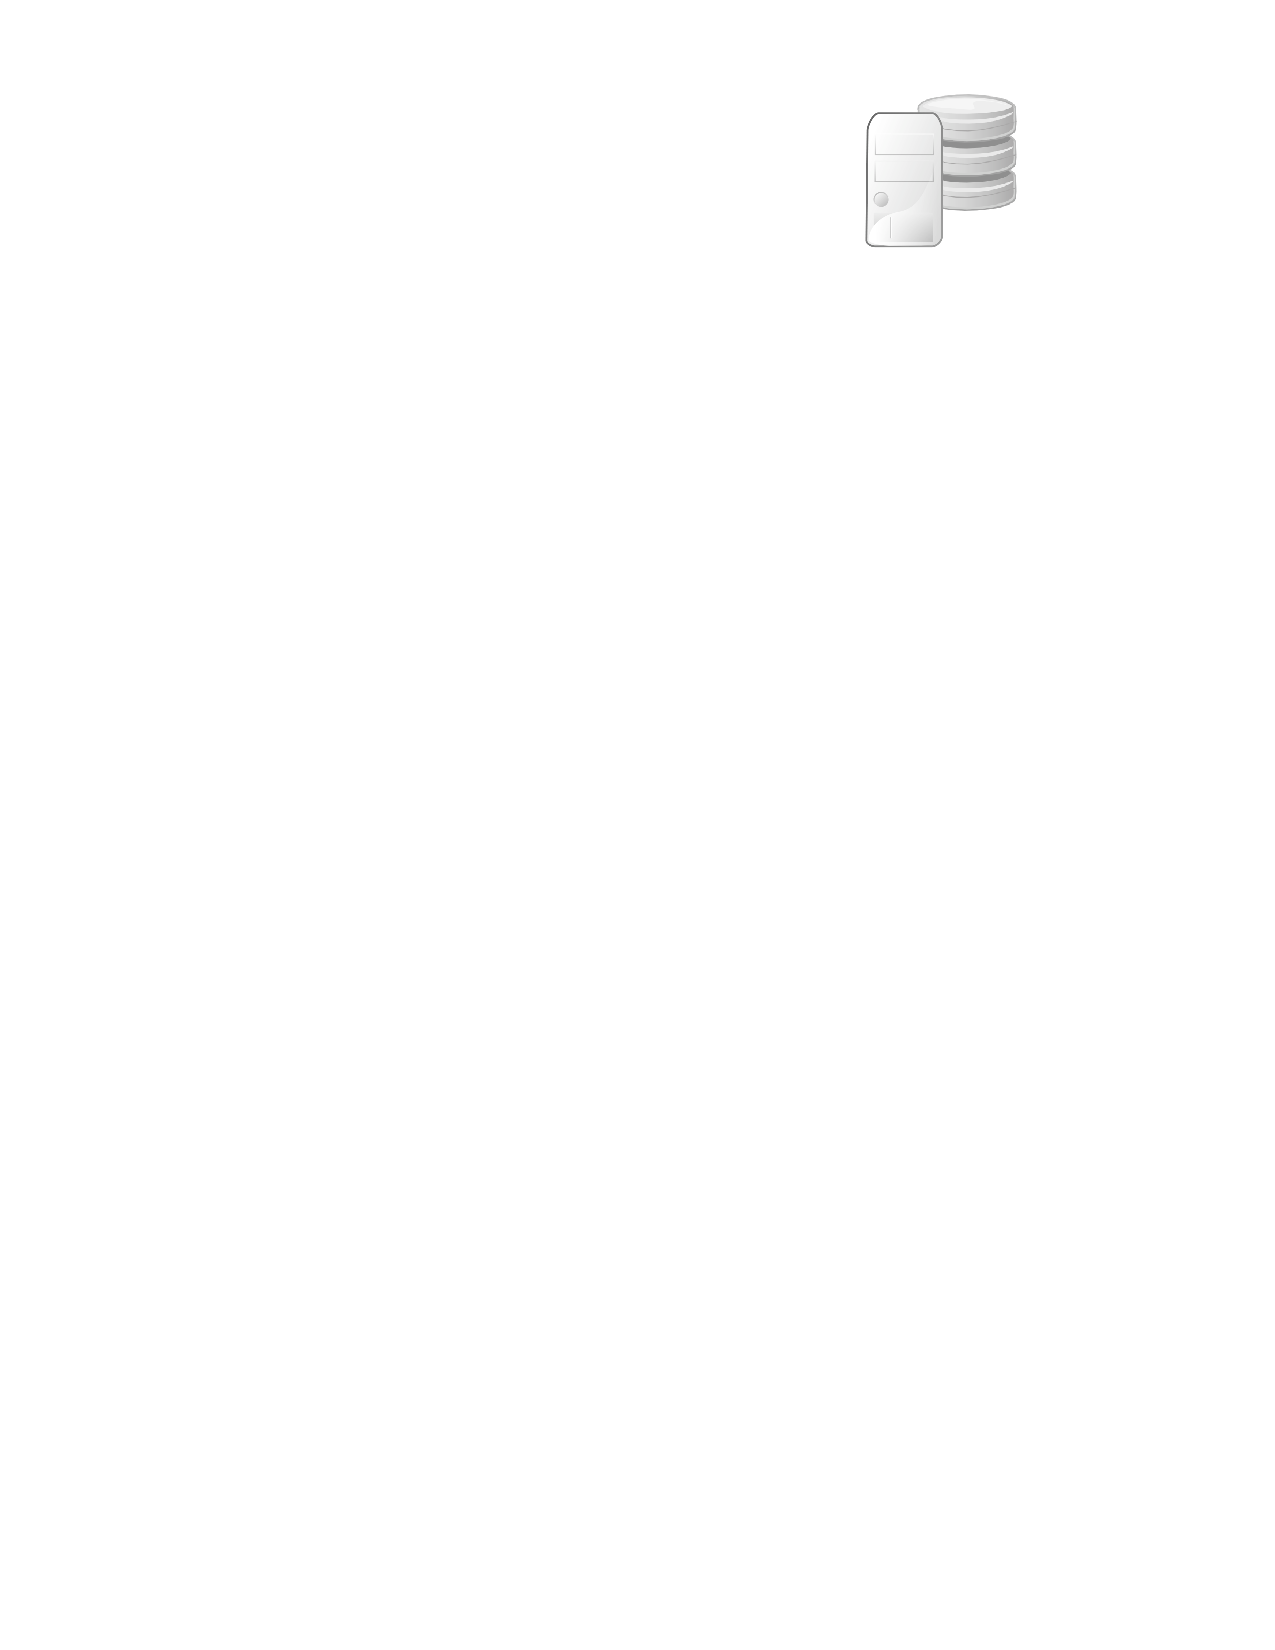
\includegraphics[height=\rinner]{figures/reposerver}\\\emph{Stratum 0 R/W}}};
	\draw[public] (0,0) circle (\router);
	
	\node[mirror] (cern) at (0,\router) {\parbox{\rmirror}{\small\centering CERN\\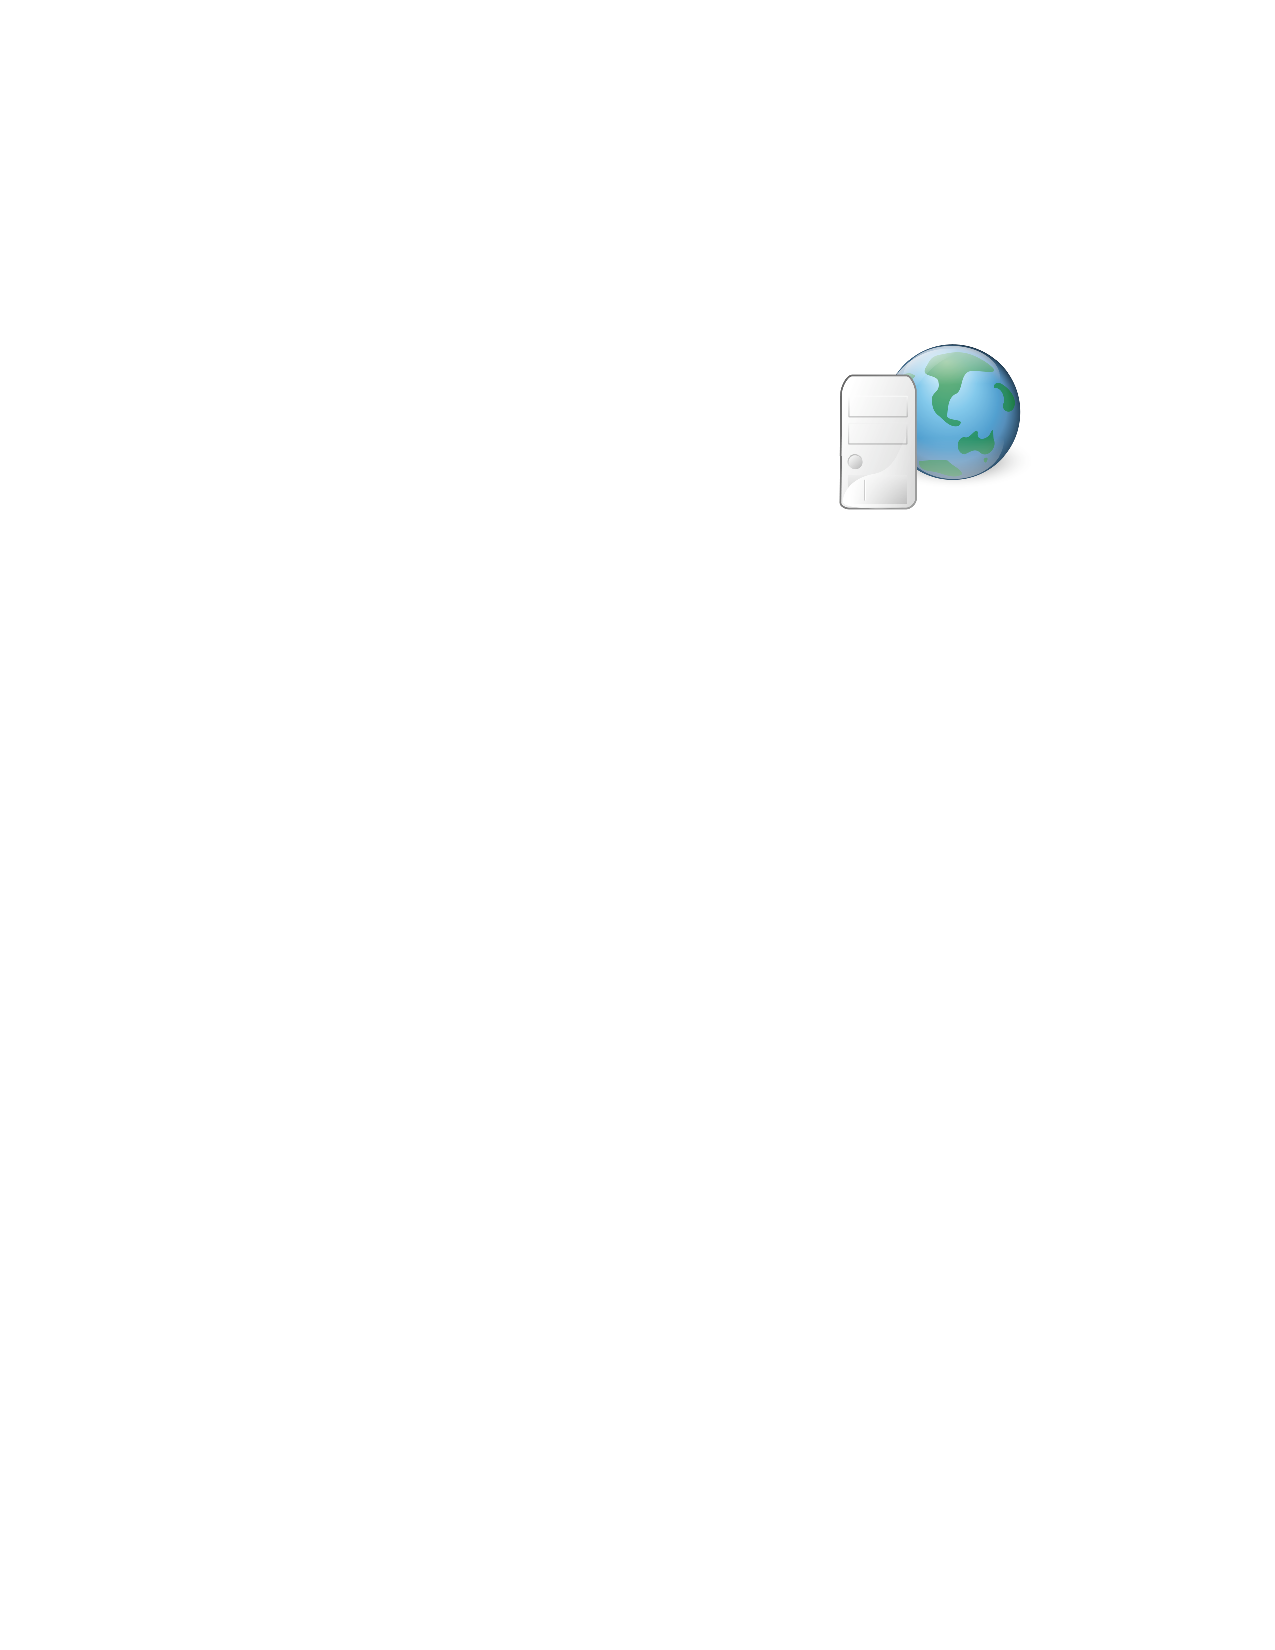
\includegraphics[height=\websize]{figures/webserver}}};
	%\draw[mirror] (cern) circle (\rmirror);
	\node[mirror] (ral) at (\router,0) {\parbox{\rmirror}{\small\centering RAL (U.K.)\\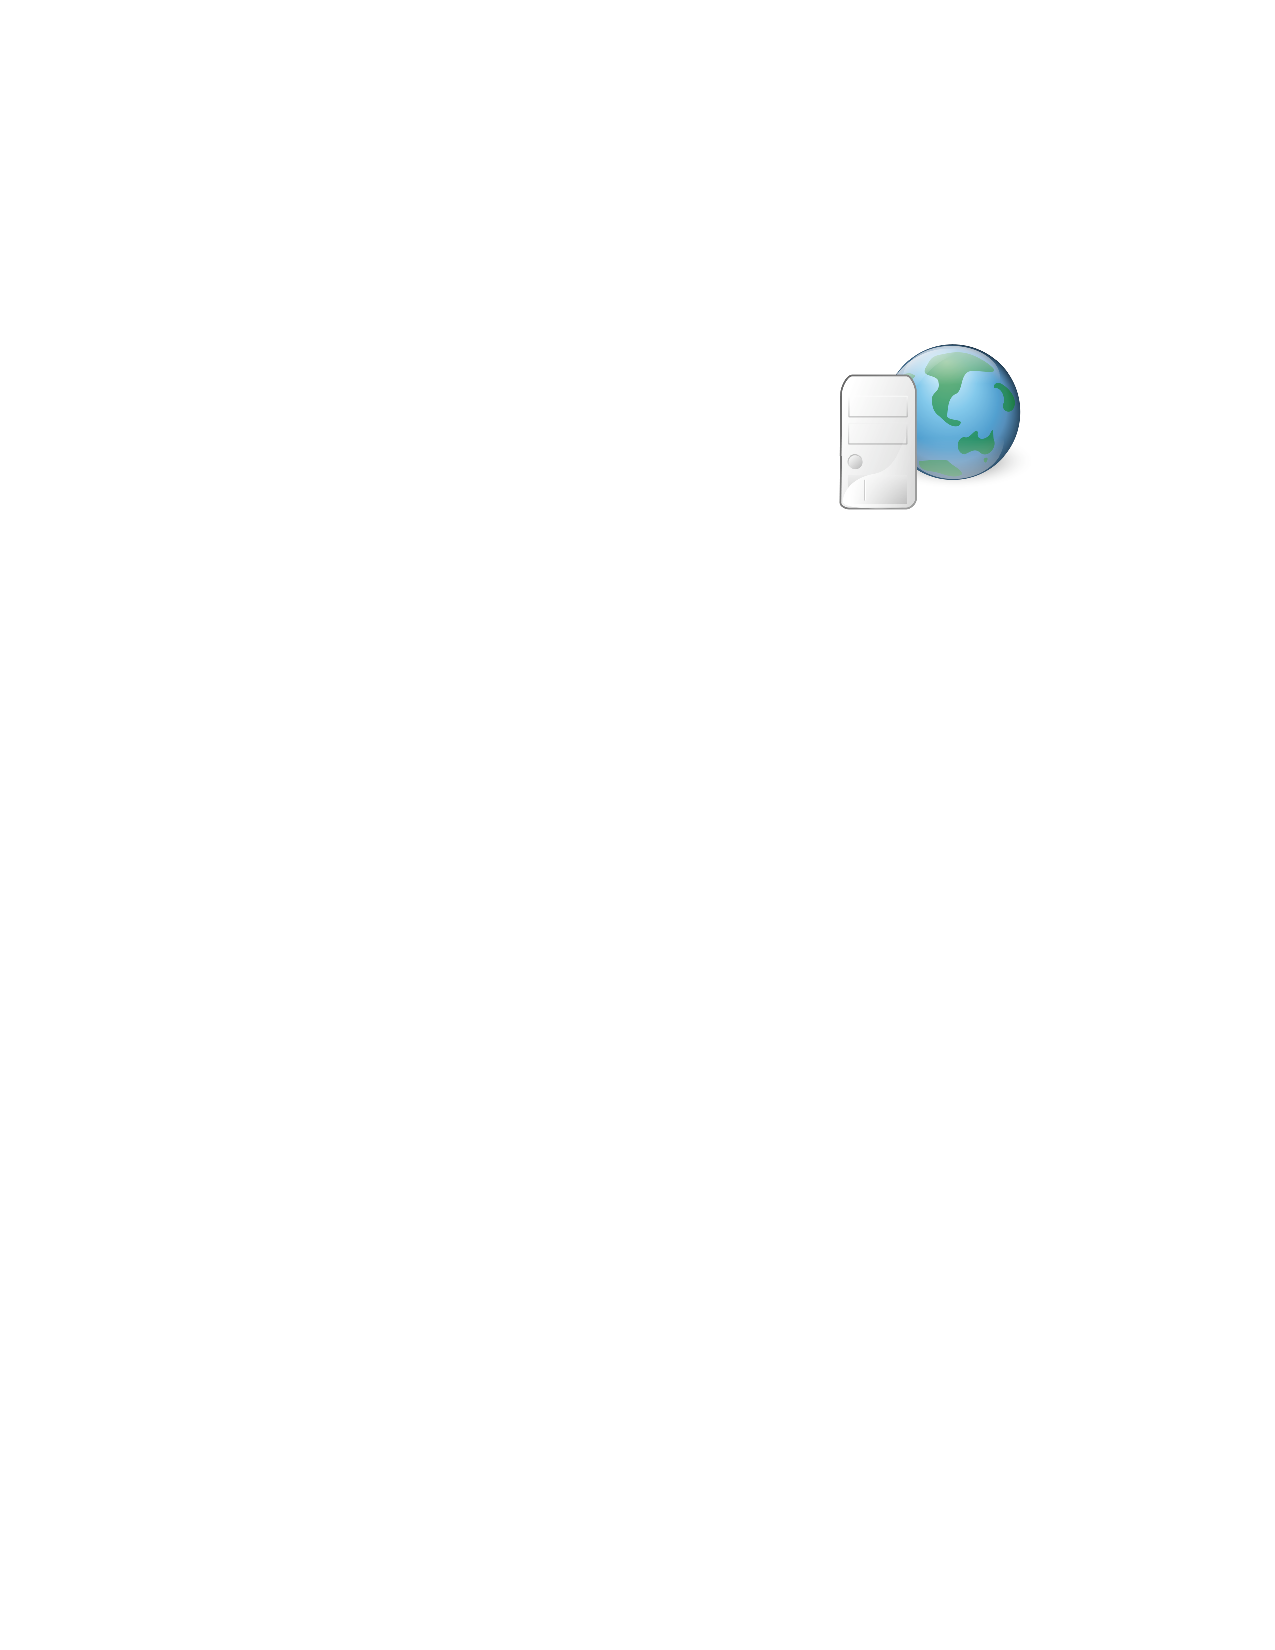
\includegraphics[height=\websize]{figures/webserver}}};
	%\draw[mirror] (ral) circle (\rmirror);
	\node[mirror] (bnl) at (-\router,0) {\parbox{\rmirror}{\small\centering FermiLab\\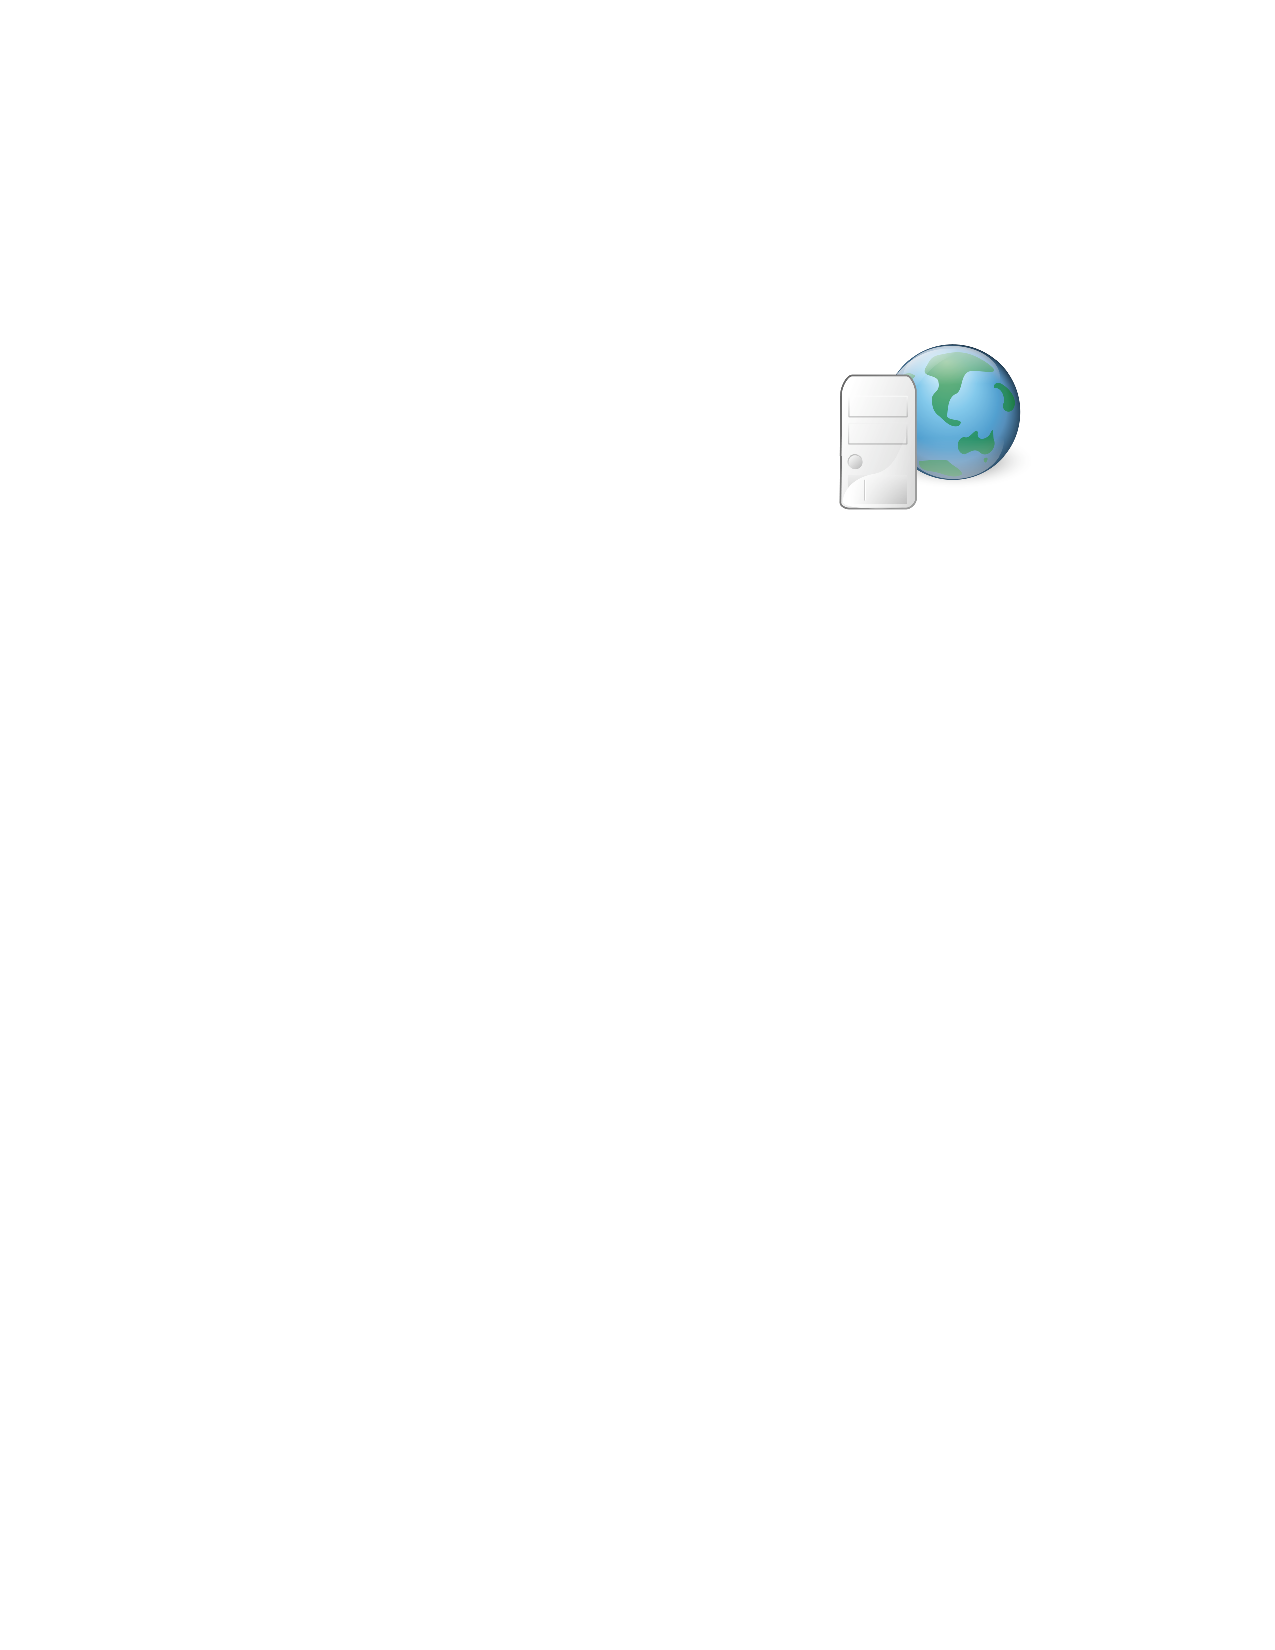
\includegraphics[height=\websize]{figures/webserver}}};
	\node[mirror] (fermilab) at (canvas polar cs:angle=225,radius=\router) {\parbox{\rmirror}{\small\centering BNL\\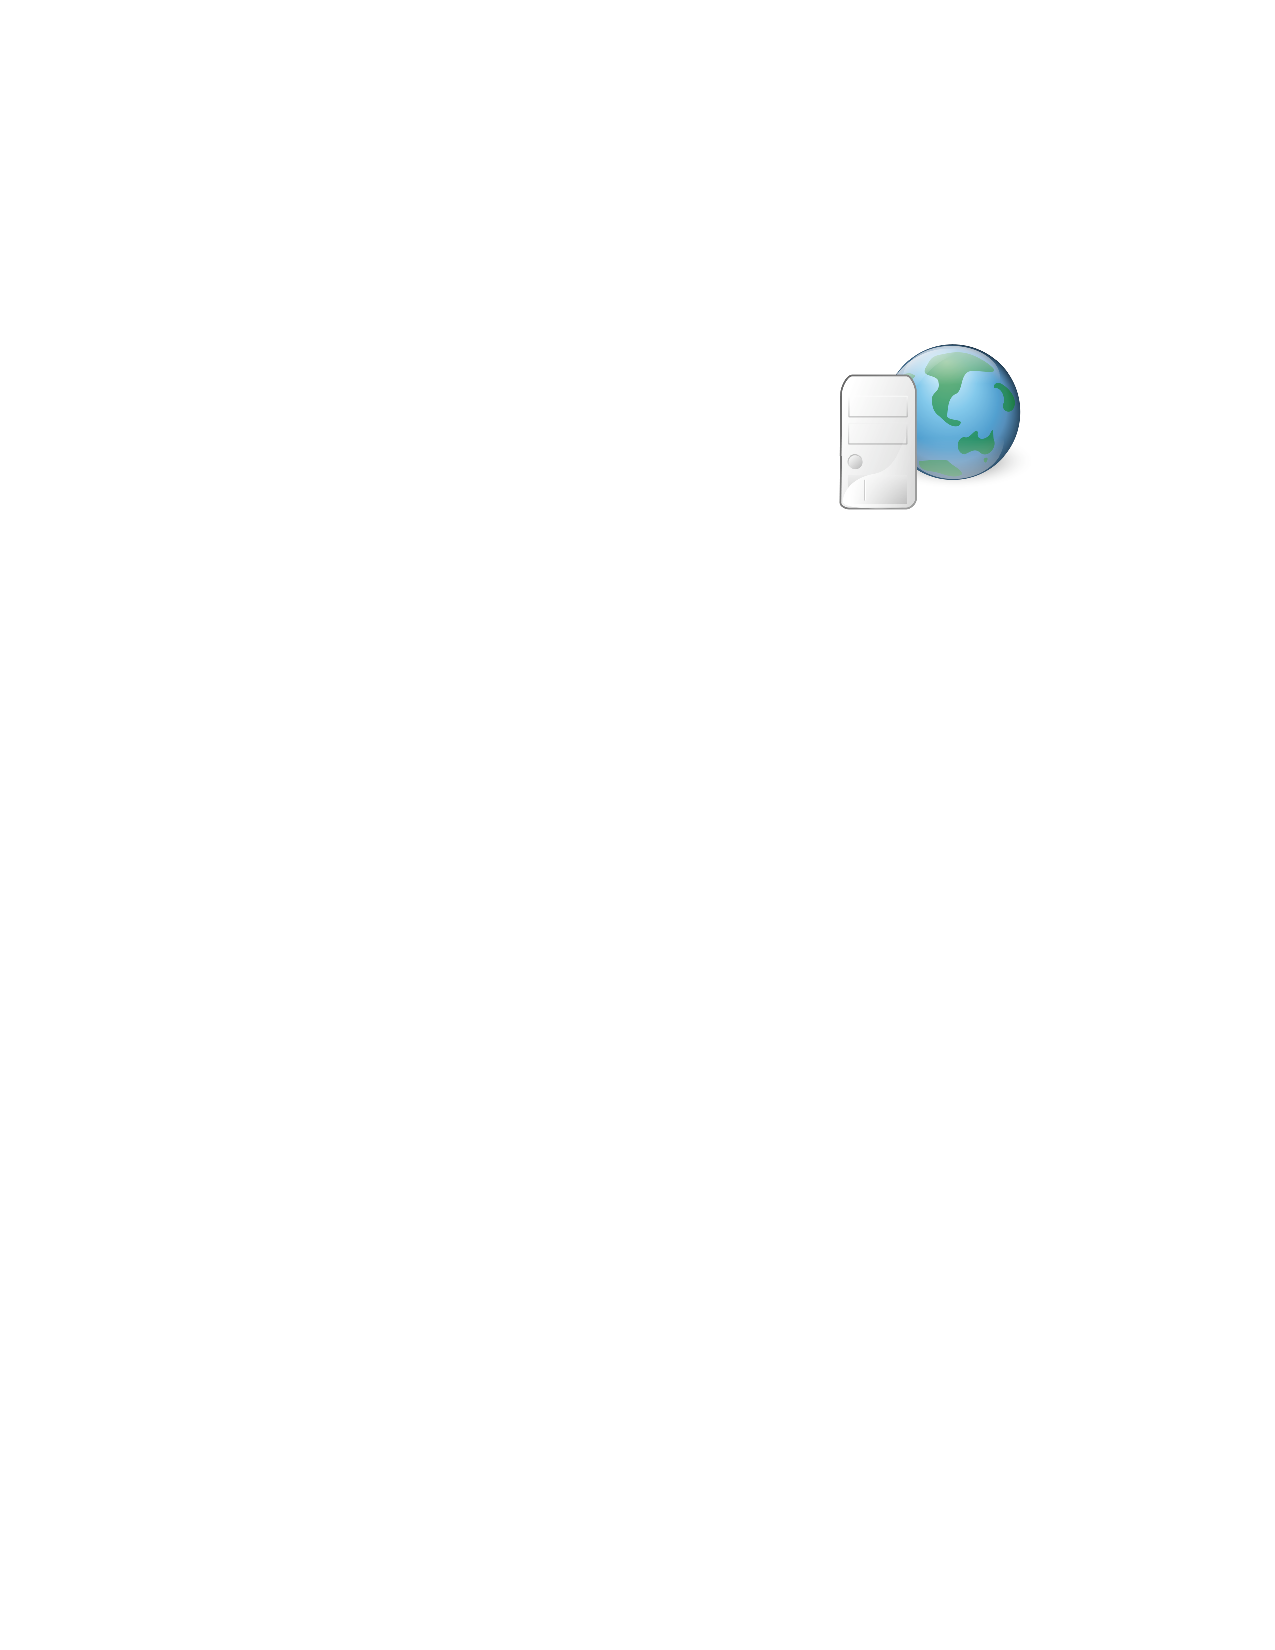
\includegraphics[height=\websize]{figures/webserver}}};
	\node[mirror] (desy) at (canvas polar cs:angle=-45,radius=\router) {\parbox{\rmirror}{\small\centering DESY\\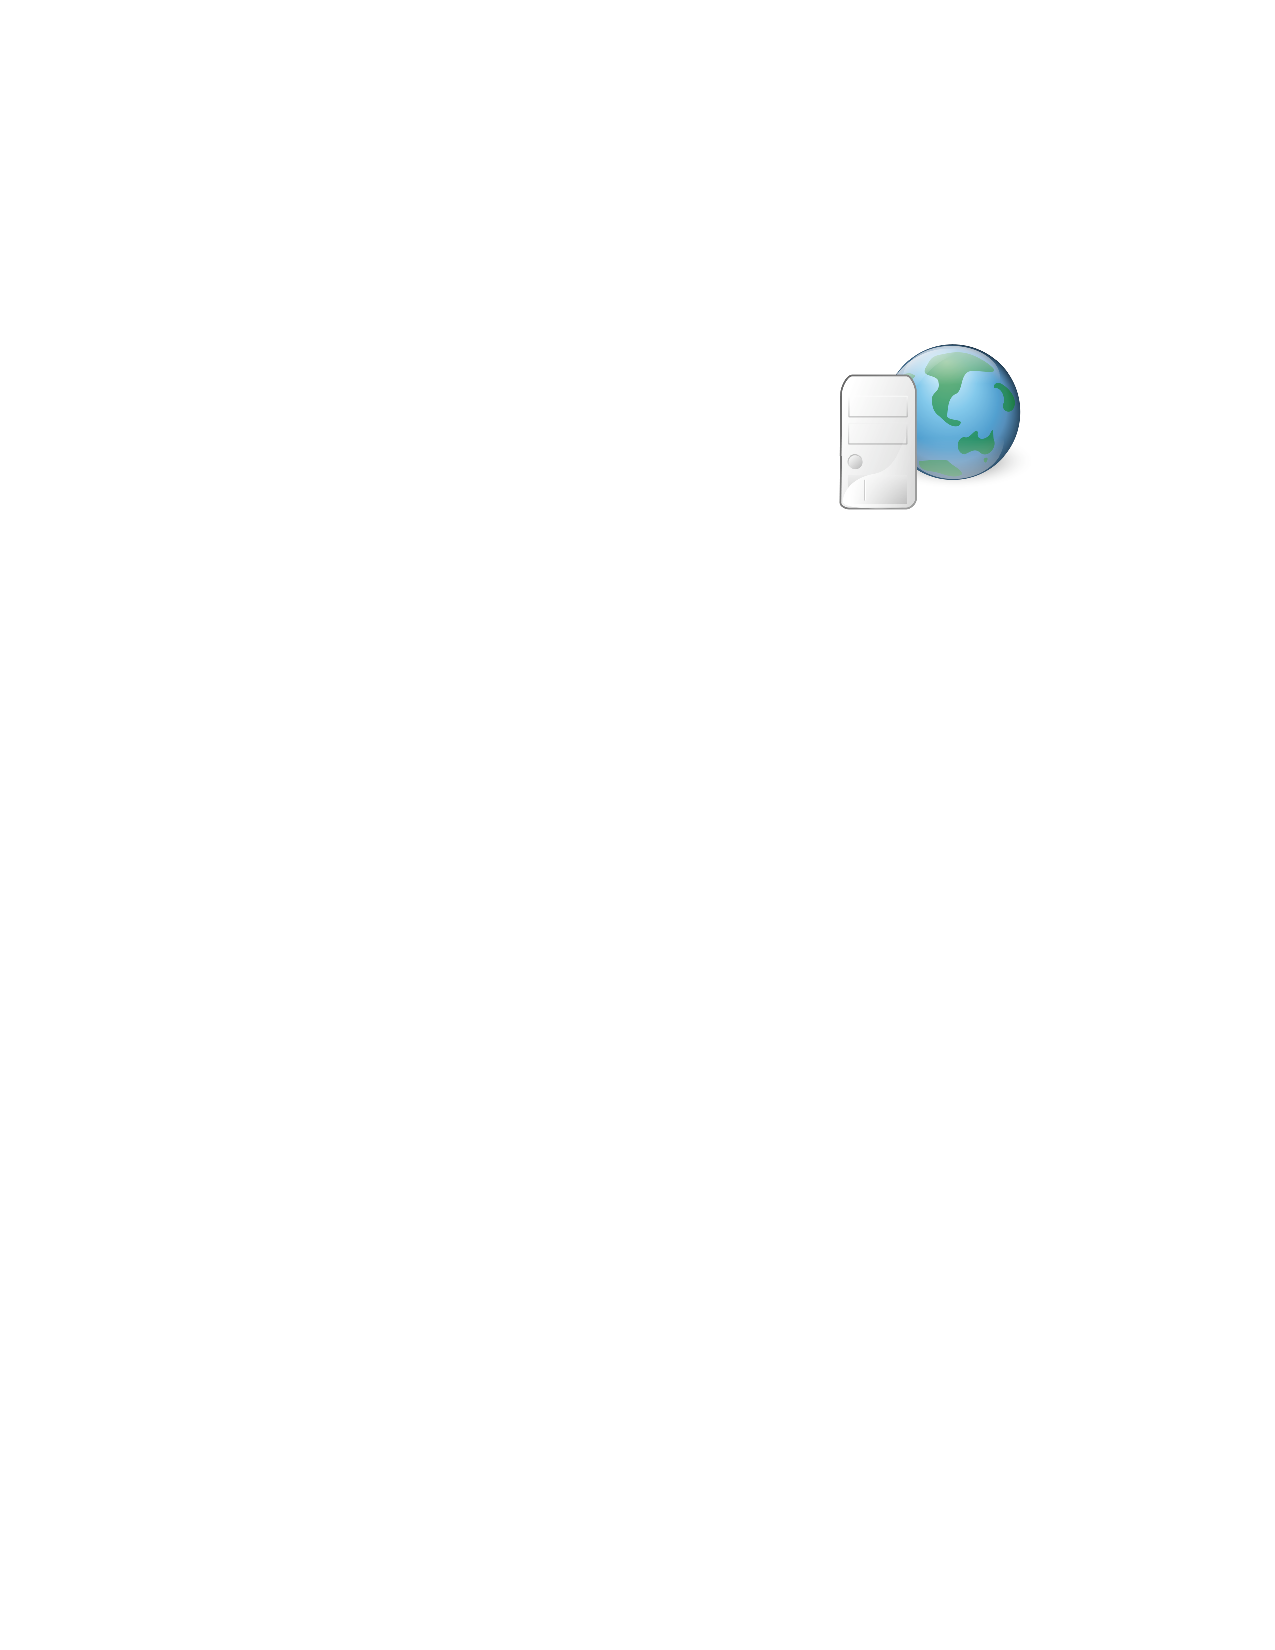
\includegraphics[height=\websize]{figures/webserver}}};
	\node[mirror] (nikhef) at (canvas polar cs:angle=45,radius=\router) {\parbox{\rmirror}{\small\centering NIKHEF\\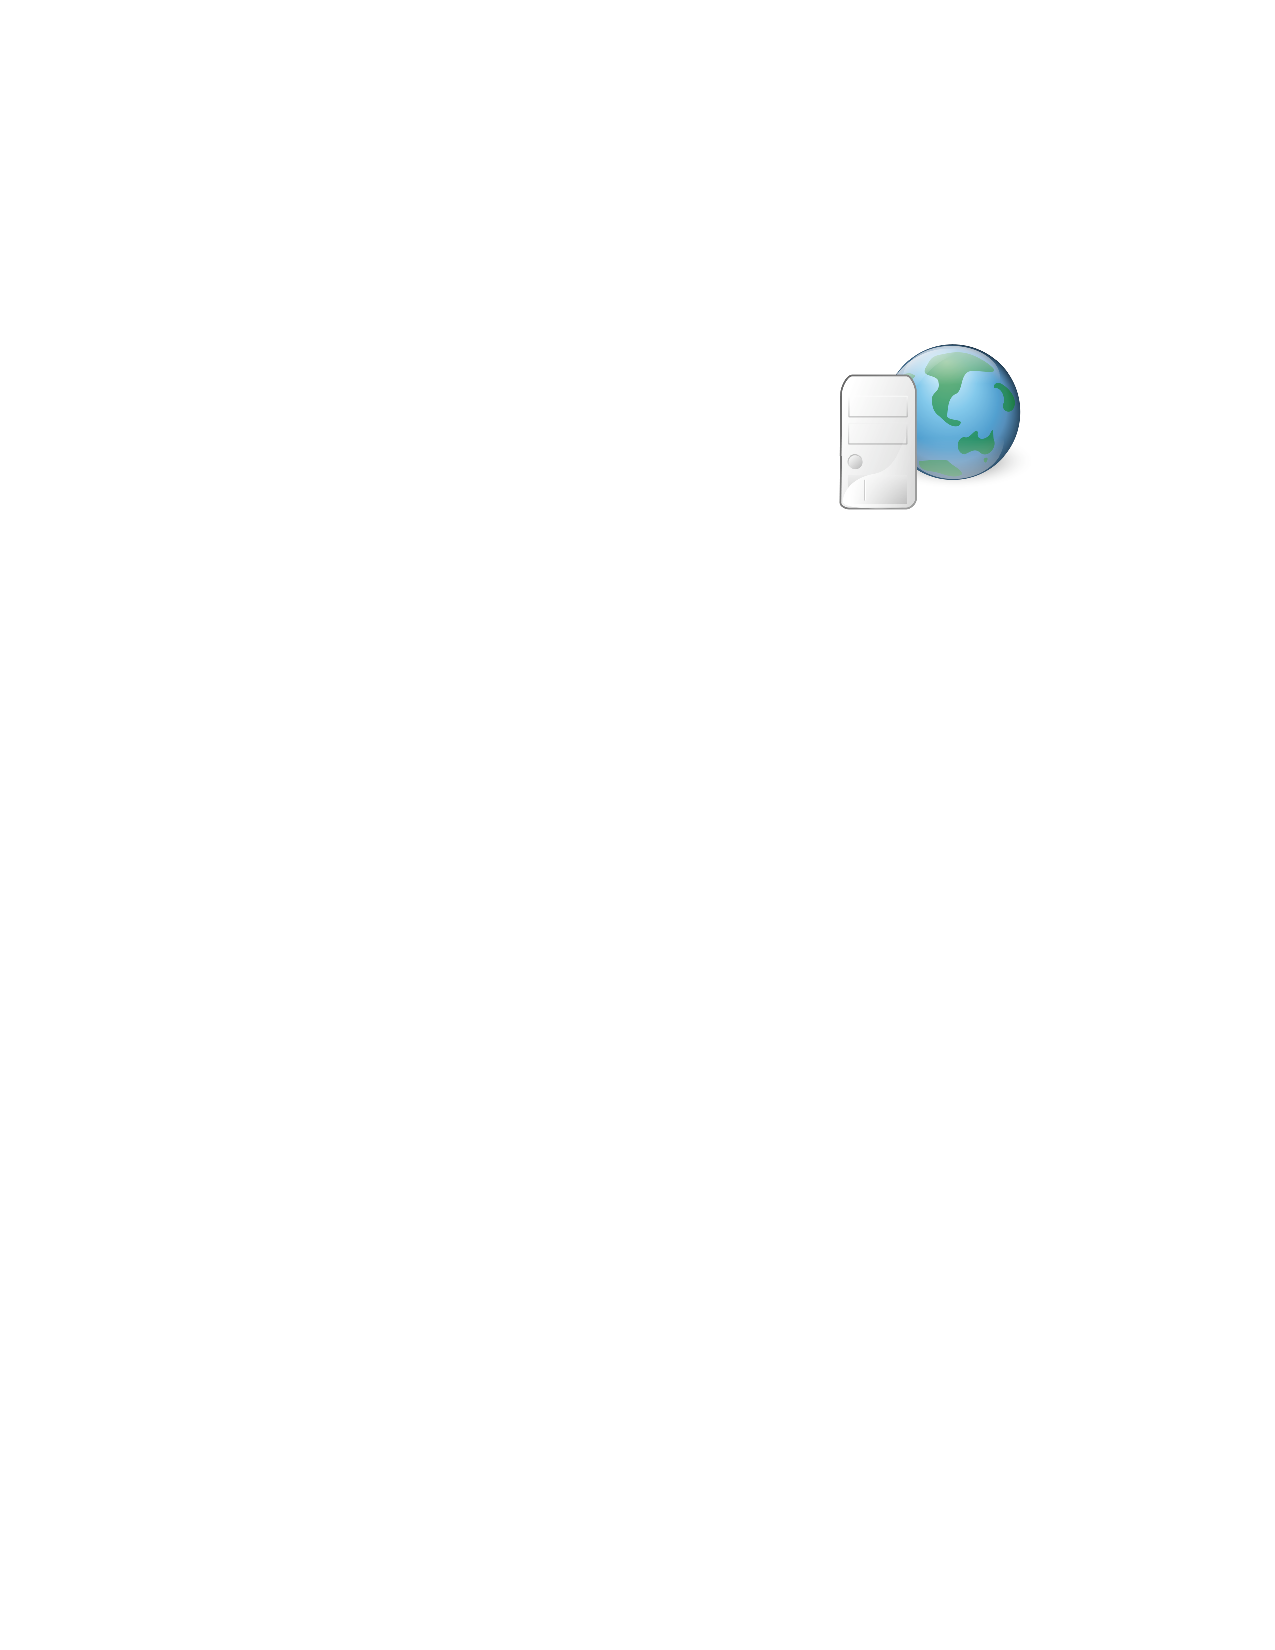
\includegraphics[height=\websize]{figures/webserver}}};
	%\draw[mirror] (bnl) circle (\rmirror);
	\node[mirror] (other) at (0,-\router) {\parbox{\rmirror}{\small\centering \emph{ASGC (Taiwan)}\\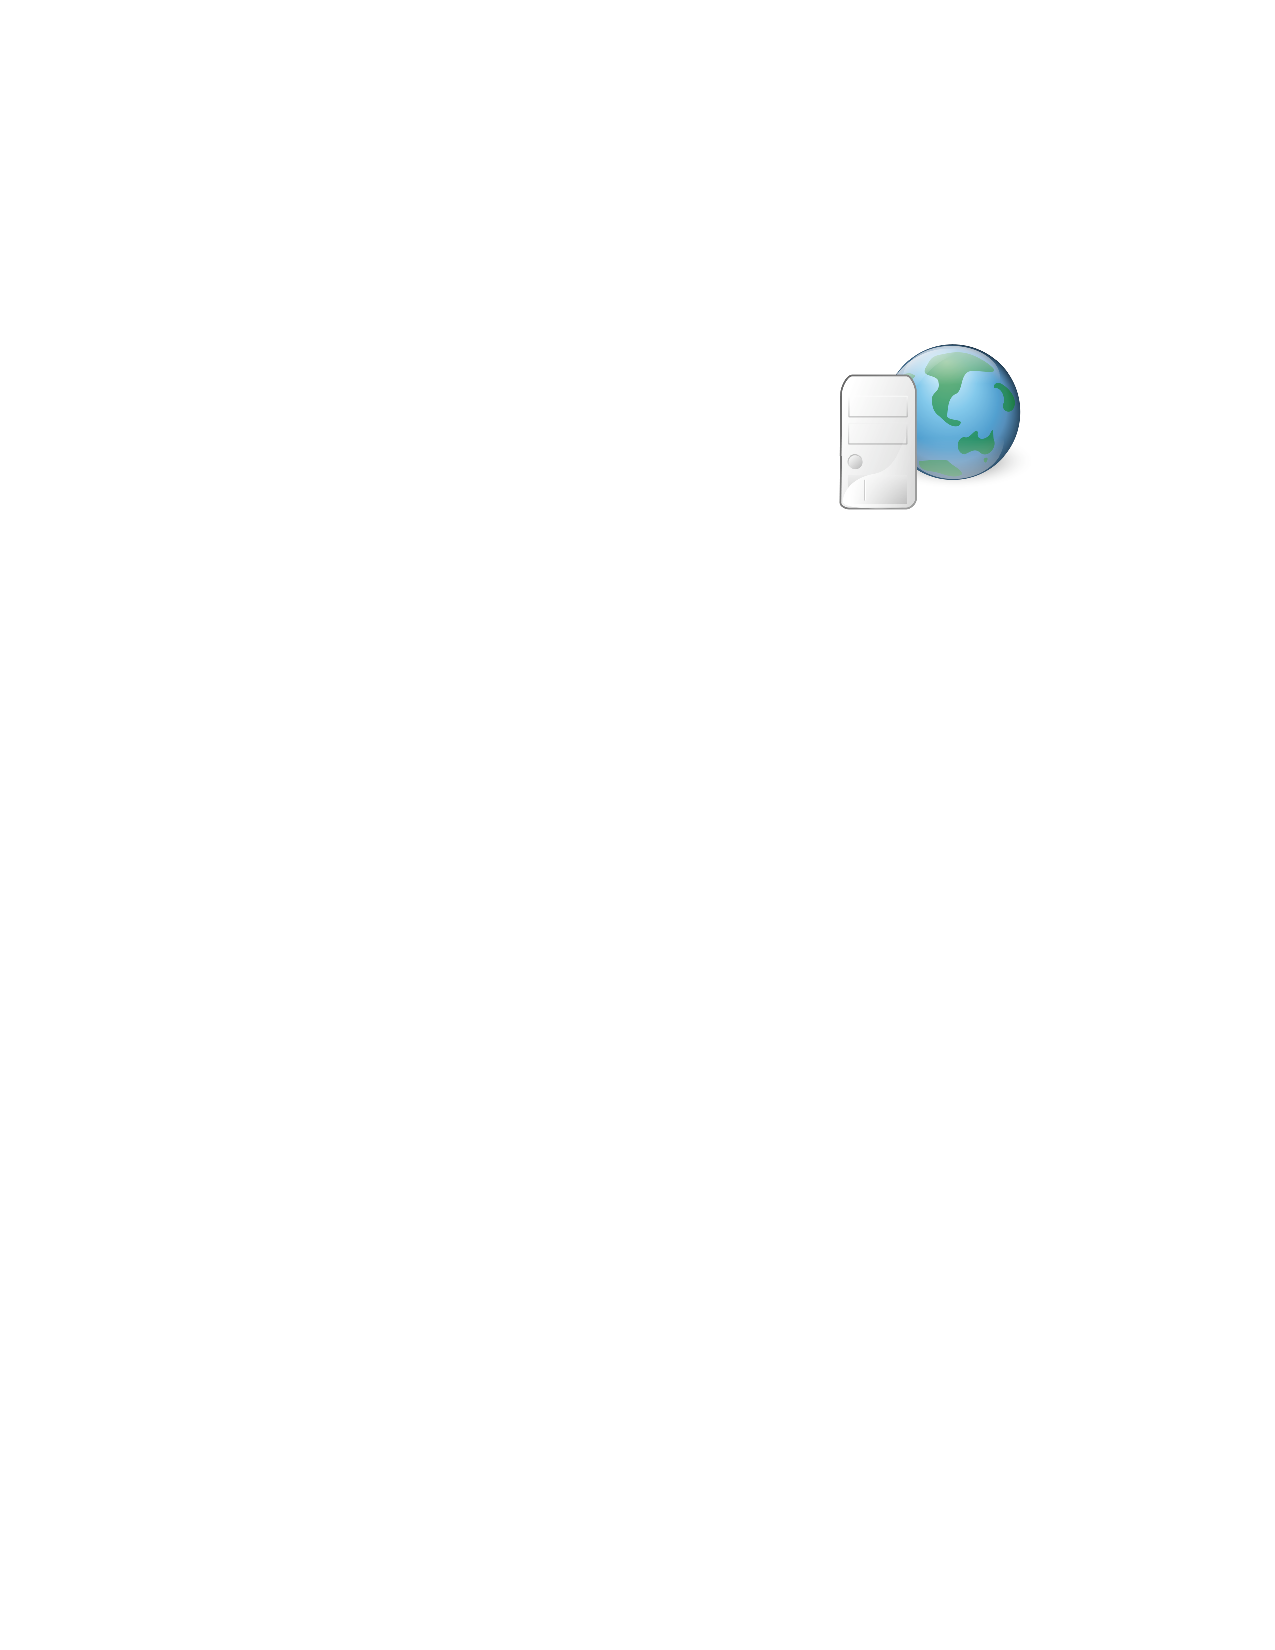
\includegraphics[height=\websize]{figures/webserver}}};
	%\draw[mirror] (other) circle (\rmirror);
	
	
	\draw[decorate,decoration={text along path,text color=blue,text={~~~~~~~~~~~~~~~~~~~|\small\it|Stratum 1||~}}] (-\router-0.3cm,0) arc (180:90:\router+0.3cm);
	\draw[decorate,decoration={text along path,text color=blue,text={~~~~~~~~~~~~~|\small|Public Mirrors||~}}] (-\router+0.5cm,0) arc (180:90:\router-0.5cm);
	%\draw (0,0) .. controls +(up:2cm) and +(left:2cm) .. (1,3) {node[public,sloped,above]{\emph{Stratum 1} Public Mirrors}};
	
	%\node[red,thick,fill=white,draw,cloud,aspect=1.5,xshift=\router+\rmirror+2cm] (tier1) {\parbox{2.2cm}{\centering\footnotesize\emph{Stratum 2}\\Private Replicas\\(Tier 1)}};
	
	\draw[replication] (rw) -- (cern);
	\draw[replication] (rw) -- (ral);
	\draw[replication] (rw) -- (bnl);
	\draw[replication] (rw) -- (fermilab);
	\draw[replication] (rw) -- (desy);
	\draw[replication] (rw) -- (nikhef);
	\draw[replication] (rw) -- (other);
	%\draw[replication,red] (ral) -- ($(tier1)-(1.8cm,0)$);
	
	\node[proxycolor,fill=white] at (-1.6*\router,0) {\parbox{1.5cm}{\centering\small Proxy\\Hierarchy}};
	\node[proxycolor,fill=white] at (1.6*\router,0) {\parbox{1.5cm}{\centering\small Proxy\\Hierarchy}};
	
\end{tikzpicture}

%\end{document}
}
	\end{center}
	\caption{\cvmfs\ content distribution network for the cern.ch domain: Stratum~1 replica servers are located in Europe, the U.S.\ and Asia.  
		One protected r/w instance (Stratum 0) is feeding up the public, distributed mirror servers. 
		A distributed hierarchy of proxy servers fetches content from the closest public mirror server.}
	\label{fig:stratum1}
\end{figure}

A Stratum~1 server is a standard web server that uses the \cvmfs\ server toolkit to create and maintain a mirror of a \cvmfs\ repository served by a Stratum~0 server.
To this end, the \texttt{cvmfs\_server} utility provides the \texttt{add-replica} command.
This command will register the Stratum~0 URL and prepare the local web server.
Periodical synchronization has to be scheduled, for instance with \texttt{cron}, using the \texttt{cvmfs\_server snapshot} command.
The advantage over general purpose mirroring tools such as \product{rSync} is that all \cvmfs\ file integrity verifications mechansims from the \fuse\ client are reused.
Additionally, by the aid of the \cvmfs\ file catalogs, the \texttt{cvmfs\_server} utility knows beforehand (without remote listing) which files to transfer.

In order to prevent accidental synchronization from a repository, the Stratum~0 repository maintainer has to create a \texttt{.cvmfs\_master\_replica} file in the HTTP root directory.
Also keep in mind that replication will thrash any caches that might be between Stratum~1 and Stratum~0.
A direct connection is therefore preferable.

\section{Recommended Setup}
The vast majority of HTTP requests will be served by the site's local proxy servers.
Being a publicly available service, however, we recommend to install caching \squid\ frontends in front of the Stratum~1 web server.
This setup is shown in Figure~\ref{fig:stratum1front}

\begin{figure}
	\centering
	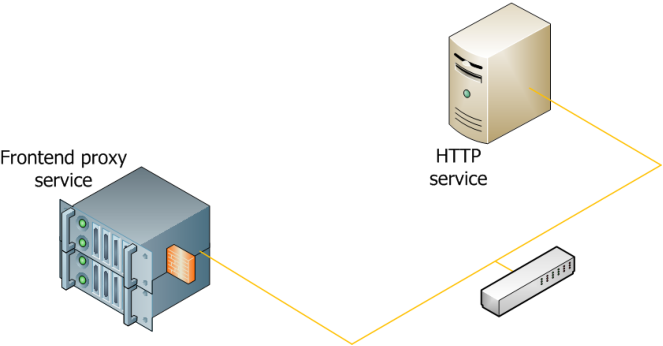
\includegraphics{figures/stratum1front}
	\caption{Recommended setup: 2 DNS load-balanced (round-robin) \squid\ machines in a reverse proxy mode in front of a single storage and web server.}
	\label{fig:stratum1front}
\end{figure}

We suggest the following key parameters:
\begin{description}
	\item[Storage.] 
		RAID-protected storage.
		The \texttt{cvmfs\_server} utility should have low latency to the storage because it runs a large number of system calls (\texttt{stat()}) against it.
		For the local storage backends ext3/4 filesystems are preferred (rather than XFS).
	\item[Web server.]
		A standard Apache server.
		Directory listing is not required.
		In addition, it is a good practice to exclude search engines from the replica web server by an appropriate robots.txt.
		The work load is mainly covered by the \squid\ servers, hence performance of the web server is not critical.
		However, the webserver should be close to the storage in terms of latency.
	\item[Squid frontend.]
		At least 2 \squid\ servers configured in load-balance mode as reverse proxies for the web server.
		The Squid frontends should listen on ports 80 and 8000.
		The more RAM \squid\ can use for caching, the better.
\end{description}

\section{Squid Configuration}
The \squid\ configuration differs from the site-local Squids because the Stratum~1 \squid\ servers are transparent to the clients (\emph{reverse proxy}).
The Squid server is configured as reverse proxy for the web server.
Concurrent requests for the same URL should be collapsed into one request to the backend.
Additionally, the cache sizes have to be set.
As the expiry rules are set by the web server, \squid\ cache expiry rules remain unchanged.

The following lines should appear accordingly in /etc/squid/squid.conf:
\begin{verbatim}
  http_port 80 accel
  http_port 8000 accel
  http_access allow all
  cache_peer <APACHE_HOSTNAME> parent 80 0 no-query originserver
  collapsed_forwarding on

  max_filedesc 8192

  cache_mem <MEM_CACHE_SIZE> MB
  cache_dir aufs /var/spool/squid <DISK_CACHE_SIZE in MB> 32 256
  maximum_object_size 1024 MB
  maximum_object_size_in_memory 8 MB
\end{verbatim}
\quad\\
Note that \texttt{http\_access allow all} has to be inserted before (or instead of) the line \texttt{http\_access deny all}.

Check the configuration syntax by \texttt{squid -k parse}.
Create the hard disk cache area with \texttt{squid -z}. 
In order to make the increased number of file descriptors effective for \squid, execute \texttt{ulimit -n 8192} prior to starting the squid service.

\section{Monitoring}
The \texttt{cvmfs\_server} utility reports status and problems to \texttt{stdout} and \texttt{stderr}.

For the infrastructure, standard \nagios\ HTTP checks do the job.
Configure it with the URL \url{http://$replica-server/cvmfs/$repository_name/.cvmfspublished}.
This file can also be used to monitor if the same repository revision is served by the Stratum~0 server and all the Stratum~1 servers.
In order to tune the hardware and cache sizes, keep an eye on the Squid server's CPU and I/O load.

Keep an eye on HTTP 404 errors.
For normal CernVM-FS traffic, such failures should not occur.
Traffic from \cvmfs\ clients is marked by an \texttt{X-CVMFS2} header.


\chapter{Implementation Notes}

\cvmfs\ has a modular structure and relies on several open source libraries.
Figure~\ref{fig:cvmfsblocks} shows the internal building blocks of \cvmfs.
Most of these libraries are shipped with the \cvmfs\ sources and are linked statically in order to facilitate debugging and to keep the system dependencies minimal.

\begin{figure}
	\begin{center}
		%\documentclass[a4paper, 11pt]{article}

%\usepackage{tikz,ifthen}
%\usetikzlibrary{shapes,matrix,shadows,fit,backgrounds}

%\begin{document}
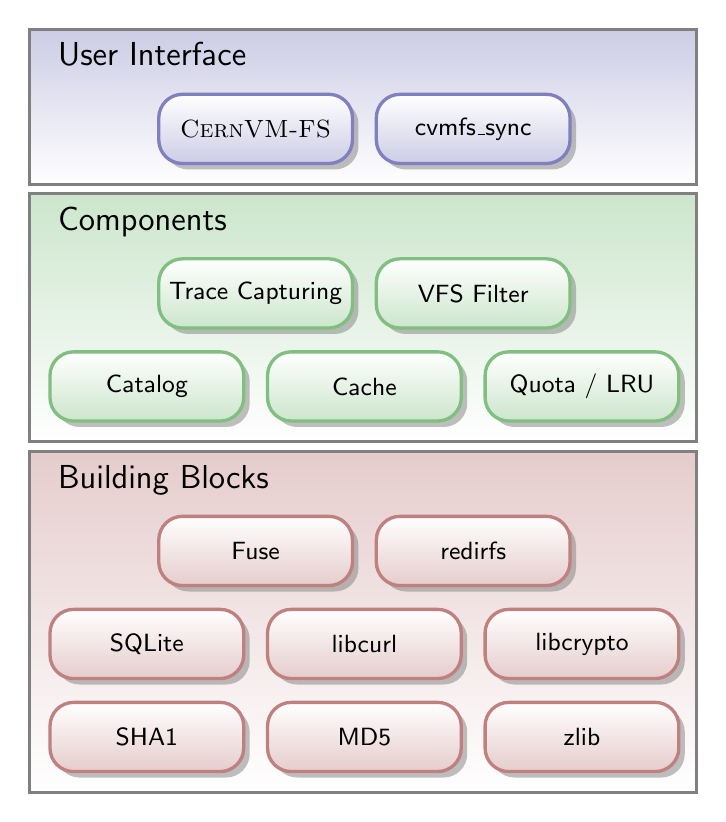
\begin{tikzpicture}
\edef\blockwidth{7em} 
\edef\blockheight{2.5em}
\scope[ 
      block/.style={
         anchor=south west,
         rectangle,
         very thick,
         drop shadow,
         rounded corners=3mm,
         minimum width=\blockwidth,
         minimum height=\blockheight},   
      buildingblock/.style={
         block,
         draw=red!50!black!50,
         top color=white,
         bottom color=red!50!black!20},
      module/.style={
         block,
         draw=green!50!black!50,
         top color=white,
         bottom color=green!50!black!20},
      fuse/.style={
         block,
         draw=blue!50!black!50,
         top color=white,
         bottom color=blue!50!black!20},
      blocklabel/.style={
         anchor=north west,
         inner ysep=-0.5ex,
         font=\large\sf},
      every fit/.style={
         rectangle,
         very thick,
         draw=gray},
      font={\small\sf}
   ]
   
   \edef\spacesep{2ex}
   \edef\numofelemsperline{3}

   % Bulding Blocks
   \edef\numofelems{8} 
   \pgfmathparse{floor(\numofelems/\numofelemsperline)*\numofelemsperline}\edef\fitsuntil{\pgfmathresult}
   \foreach \i / \name in {0 / SHA1, 1 / MD5, 2 / zlib, 3 / SQLite, 4 / libcurl, 5 / libcrypto, 6 / Fuse, 7 / redirfs}
   {
      \ifthenelse{\i<\fitsuntil}{\edef\offset{0}}{
         \pgfmathparse{((\numofelemsperline-mod(\numofelems,\numofelemsperline))/2)*(\blockwidth+\spacesep)}\edef\offset{\pgfmathresult}}
      \pgfmathparse{\offset + mod(\i,\numofelemsperline)*(\blockwidth+\spacesep)}\edef\blockx{\pgfmathresult}
      \pgfmathparse{floor(\i/\numofelemsperline) * (\blockheight+\spacesep)}\edef\blocky{\pgfmathresult}
      \coordinate (blockxy) at (\blockx pt, \blocky pt);
      \node [buildingblock] at (blockxy) {\name};
   }
   \pgfmathparse{\numofelemsperline*(\blockwidth+\spacesep)-\spacesep}\edef\extremx{\pgfmathresult}
   \pgfmathparse{ceil(\numofelems/\numofelemsperline)*(\blockheight+\spacesep)-\spacesep + 4ex}\edef\extremy{\pgfmathresult}
   \coordinate (extremxy) at (\extremx pt, \extremy pt);
   \node (bb bottom left) at (0,0) {};
   \node (bb top right) at (extremxy) {};
   \begin{pgfonlayer}{background}
      \node [fit=(bb bottom left) (bb top right),top color=red!50!black!20,bottom color=white] (bb box) {};
      \node [blocklabel] at (0,\extremy pt) {Building Blocks};
   \end{pgfonlayer}
   

   % Modules
   \pgfmathparse{\extremy+2*\spacesep}\edef\yoffset{\pgfmathresult}
   \edef\numofelems{5}
   \pgfmathparse{floor(\numofelems/\numofelemsperline)*\numofelemsperline}\edef\fitsuntil{\pgfmathresult}
   \foreach \i / \name in {0 / Catalog, 1 / Cache, 2 / {Quota / LRU}, 3 / Trace Capturing, 4 / {VFS Filter}}
   {
      \ifthenelse{\i<\fitsuntil}{\edef\offset{0}}{
         \pgfmathparse{((\numofelemsperline-mod(\numofelems,\numofelemsperline))/2)*(\blockwidth+\spacesep)}\edef\offset{\pgfmathresult}}
      \pgfmathparse{\offset + mod(\i,\numofelemsperline)*(\blockwidth+\spacesep)}\edef\blockx{\pgfmathresult}
      \pgfmathparse{\yoffset + floor(\i/\numofelemsperline) * (\blockheight+\spacesep)}\edef\blocky{\pgfmathresult}
      \coordinate (blockxy) at (\blockx pt, \blocky pt);
      \node [module] at (blockxy) {\name};
   }
   \pgfmathparse{\numofelemsperline*(\blockwidth+\spacesep)-\spacesep}\edef\extremx{\pgfmathresult}
   \pgfmathparse{\yoffset+ceil(\numofelems/\numofelemsperline)*(\blockheight+\spacesep)-\spacesep + 4ex}\edef\extremy{\pgfmathresult}
   \coordinate (extremxy) at (\extremx pt, \extremy pt);
   \node (mod bottom left) at (0,\yoffset pt) {};
   \node (mod top right) at (extremxy) {};
   \begin{pgfonlayer}{background}
      \node [fit=(mod bottom left) (mod top right),top color=green!50!black!20,bottom color=white] (mod box) {};
      \node [blocklabel] at (0,\extremy pt) {Components};
   \end{pgfonlayer}
   
   %fuse
   \pgfmathparse{\extremy+2*\spacesep}\edef\yoffset{\pgfmathresult}
   \edef\numofelems{2}
   \pgfmathparse{floor(\numofelems/\numofelemsperline)*\numofelemsperline}\edef\fitsuntil{\pgfmathresult}
   \foreach \i / \name in {0 / \cvmfs, 1 / cvmfs\_sync}
   {
      \ifthenelse{\i<\fitsuntil}{\edef\offset{0}}{
         \pgfmathparse{((\numofelemsperline-mod(\numofelems,\numofelemsperline))/2)*(\blockwidth+\spacesep)}\edef\offset{\pgfmathresult}}
      \pgfmathparse{\offset + mod(\i,\numofelemsperline)*(\blockwidth+\spacesep)}\edef\blockx{\pgfmathresult}
      \pgfmathparse{\yoffset + floor(\i/\numofelemsperline) * (\blockheight+\spacesep)}\edef\blocky{\pgfmathresult}
      \coordinate (blockxy) at (\blockx pt, \blocky pt);
      \node [fuse] at (blockxy) {\name};
   }
   \pgfmathparse{\numofelemsperline*(\blockwidth+\spacesep)-\spacesep}\edef\extremx{\pgfmathresult}
   \pgfmathparse{\yoffset+ceil(\numofelems/\numofelemsperline)*(\blockheight+\spacesep)-\spacesep + 4ex}\edef\extremy{\pgfmathresult}
   \coordinate (extremxy) at (\extremx pt, \extremy pt);
   \node (fuse bottom left) at (0,\yoffset pt) {};
   \node (fuse top right) at (extremxy) {};
   \begin{pgfonlayer}{background}
      \node [fit=(fuse bottom left) (fuse top right),top color=blue!50!black!20,bottom color=white] (fuse box) {};
      \node [blocklabel] at (0,\extremy pt) {User Interface};
   \end{pgfonlayer}      
\endscope
\end{tikzpicture}
%\end{document}

	\end{center}
	\caption{\cvmfs\ block diagram.}
	\label{fig:cvmfsblocks}
\end{figure}


\section{File Catalog}

A \cvmfs\ repository is defined by its \emph{file catalog}.
The file catalog is an \sqlite\footnote{\url{https://www.sqlite.org}} database~\cite{sqlite10} having a single table that lists files and directories together with its metadata.
The table layout is shown in Table~\ref{tab:catalog}.

\begin{table}
	\begin{center}
		\begin{tabular}[b]{ccc}
			\begin{tabular}{ll}
				\toprule
				\bf Field & \bf Type \\
				\midrule
				\bf Path MD5		& 128\,Bit Integer \\
				Parent Path MD5		& 128\,Bit Integer \\
				Hardlinks			& Integer \\
				SHA1 Content Hash	& 160\,Bit Integer \\
				Size 				& Integer\\
				Mode 				& Integer \\
				Last Modified 		& Timestamp \\
				Flags 				& Integer \\
				Name 				& String \\
				Symlink 			& String \\
				uid 				& Integer \\
				gid 				& Integer \\
				\bottomrule
			\end{tabular} &
			\qquad & 
			\begin{tabular}{ll}
				\toprule
				\bf Flags & \bf Meaning\\
				\midrule
				1		& Directory \\
				2		& Transition point to a nested catalog \\
				33		& Root directory of a nested catalog \\
				3		& Regular file \\
				4		& Symbolic link \\
				\bottomrule
			\end{tabular}
		\end{tabular}
	\end{center}
	\caption{Metadata information stored per directory entry.  
		The inode is dynamically issued by \cvmfs\ at runtime.}
	\label{tab:catalog}
\end{table}

In order to save space we do not store absolute paths.
Instead we store MD5~\cite{rfc1321,rfc6151} hash values of the absolute path names.
Symbolic links are kept in the catalog.
Symbolic links may contain environment variables in the form \texttt{\$(VAR\_NAME)} that will be dynamically resolved by \cvmfs\ on access.
Hardlinks are emulated by \cvmfs.
The hardlink count is stored in the lower 32bit of the hardlinks field, a \emph{hardlink group} is stored in the higher 32 bit.
If the hardlink group is greater than zero, all files with the same hardlink group will get the same inode issued by the \cvmfs\ Fuse client.
The emulated hardlinks work within the same directory, only.
The SHA-1~\cite{rfc3175} content hash referrs to the zlib-compressed~\cite{rfc1950} version of the file.
Flags indicate the type of an directory entry (see Table~\ref{tab:catalog}).

A file catalog contains a \emph{time to live} (TTL), stored in seconds.
The catalog TTL advises clients to check for a new version of the catalog, when expired.
Checking for a new catalog version takes place with the first file system operation on a \cvmfs\ volume after the TTL has expired.
The default TTL is one hour.
If a new catalog is available, \cvmfs\ delays it's loading for the period of the \cvmfs\ kernel cache life time (default: 1 minute).
During this drain-out period, the kernel caching is turned off.
The first file system operation on a \cvmfs\ volume after that additional delay will apply a new file catalog and kernel caching is turned back on.

\subsection{Nested Catalogs}
In order to keep catalog sizes reasonable\footnote{As a rule of thumb, file catalogs up to \SI{25}{\mega\byte} (compressed) are reasonably small.}, repository subtrees may be cut and stored as separate \emph{nested catalogs}.
There is no limit on the level of nesting.
A reasonable approach is to store separate software versions as separate nested catalogs.
Figure~\ref{fig:nested} shows the directory structure which we use for the ATLAS repository.
\begin{figure}
	\begin{center}
		\framebox{%\documentclass[a4paper, 11pt]{article}

%\include{jtex}
%\usepackage{tikz,ifthen}
%\usetikzlibrary{arrows,positioning,shapes,topaths,calc,fit,backgrounds,matrix,shadows}

%\begin{document}

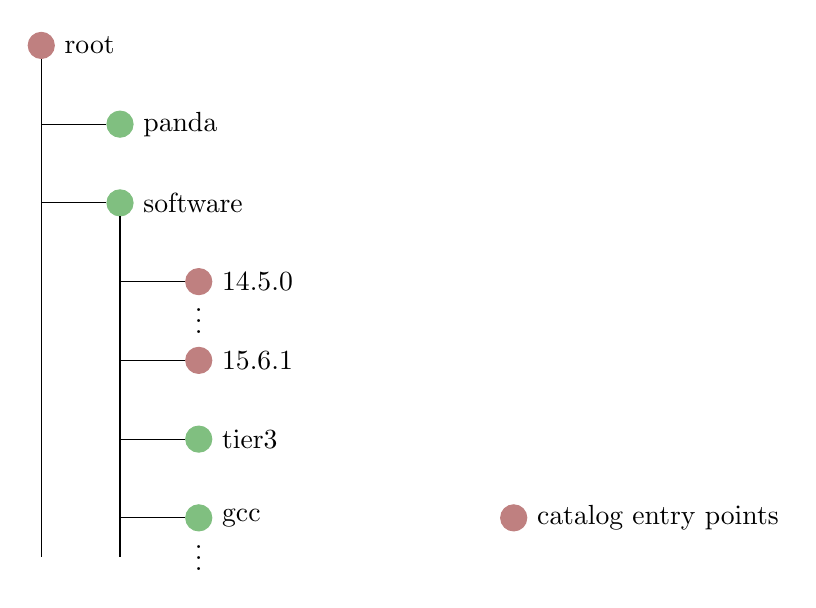
\begin{tikzpicture}
	[
		dirent/.style={
			circle,
			draw=green!50!black!50,
			fill=green!50!black!50
		}
	]
	\node[dirent,label=right:root,red!50!black!50,fill=red!50!black!50] (root) at (0,0) {};
	\node[dirent,label=right:panda] (panda) at (1, -1) {};
	\node[dirent,label=right:software] (software) at (1, -2) {};
	\node[dirent,label=right:14.5.0,red!50!black!50,fill=red!50!black!50] (1450) at (2, -3) {};
	\node[] (dots1) at (2, -3.4) {$\vdots$};
	\node[dirent,label=right:15.6.1,red!50!black!50,fill=red!50!black!50] (1561) at (2, -4) {};
	\node[dirent,label=right:tier3] (tier3) at (2, -5) {};
	\node[dirent,label=right:gcc] (gcc) at (2, -6) {};
	\node[] (dots2) at (2, -6.4) {$\vdots$};
	\node[dirent,label=right:catalog entry points,red!50!black!50,fill=red!50!black!50] (key) at (6,-6) {};
	
	%\node[dirent] (d2) at (0.4, 0.8) {};
	%\node[dirent,red!50!black!50,fill=red!50!black!50] (d21) at (0.8, 0.4) {};
	%\node[dirent] (d22) at (0.8, 0) {};
	%\node[scale=0.175] (file) at (2, 0.8) {\pdfimage{file.pdf}};
	
	\draw (root) -- (0,-1) -- (panda);
	\draw (0,-1) -- (0,-2) -- (software);
	\draw (0,-2) -- (0,-6.5);
	\draw (software) -- (1,-3) -- (1450);
	\draw (1,-3) -- (1,-4) -- (1561);
	\draw (1,-4) -- (1,-5) -- (tier3);
	\draw (1,-5) -- (1,-6) -- (gcc);
	\draw (1,-6) -- (1,-6.5);
\end{tikzpicture}
%\end{document}}
	\end{center}
	\caption{Directory structure useds for the ATLAS repository (simplified).}
	\label{fig:nested}
\end{figure}

When a subtree is moved into a nested catalog, its entry directory serves as \emph{transition point} for nested catalogs.
This directory appears as empty directory in the parent catalog with flags set to 2.
The same path appears as root-directory in the nested catalog with flags set to 33.
Because the MD5 hash values refer to full absolute paths, nested catalogs store the root path prefix.
This prefix is prepended transparently by \cvmfs.
The SHA-1 key of nested catalogs is stored in the parent catalog.
Therefore, the root catalog fully defines an entire repository.

Loading of nested catalogs happens on demand by \cvmfs\ on the first attempt to access of anything inside, \ie a user won't see the difference between a single large catalog and several nested catalogs.
While this usually avoids unnecessary catalogs to be loaded, recursive operations like \texttt{find} can easily bypass this optimization.

\subsection{Catalog Statistics}
A \cvmfs\ file catalog maintains several counters about its contents and the contents of all of its nested catalogs. 
The idea is that the catalogs know how many entries there are in their sub catalogs even without opening them.
This way, one can immediately tell how many entries, for instance, the entire ATLAS repository has. 
The numbers are shown using the number of inodes in \texttt{statvfs}. 
So \texttt{df -i} shows the overall number of entries in the repository and (as number of used inodes) the number of entries of currently loaded catalogs. 
Nested catalogs create an additional entry (the transition directory is stored in both the parent and the child catalog). 
File hardlinks are still individual entries (inodes) in the cvmfs catalogs.
The following counters are maintained for both a catalog itself and for the subtree this catalog is root of:
\begin{itemize}
	\item Number of regular files
	\item Number of symbolic links
	\item Number of directories
	\item Number of nested catalogs
\end{itemize}

%\subsection{$\mu$-Catalogs}
%The $\mu$-catalogs can be constructed in addition to the normal file catalogs.
%The $\mu$-catalogs can be considered as a special case of nested catalogs, in which each directory is a nested catalog.
%Essentially they are a precalculated \texttt{ls -la} for all directories.
%They are implemented as SQlite catalogs as well having the same structure as normal catalogs.
%The SHA-1 content hashes of the $\mu$-catalogs are stored in the hash field of the directory entries in the catalog table.


\subsection{Catalog Signature}
In order to provide authoritative information about a repository publisher, file catalogs are signed by an X.509 certificate.
The \cvmfs\ server tool kit uses a X.509 certificate together with its private key in order to sign a catalog and its nested catalogs.
It is important to note that it is sufficient to sign just the file catalog.
Since every file is listed with its SHA-1 content hash inside the catalog, we gain a secure chain and may speak of a ``signed repository''.

In order to validate file catalog signatures, \cvmfs\ uses a white-list of valid publisher certificates.
The white-list contains the SHA-1 fingerprints of known publisher certificates and a timestamp.
A white-list is valid for 30 days.
It is signed by a private RSA key, which we refer to as \emph{master key}.
%For the cern.ch repositories, the master key is kept offline on a secure smart card at \cern.
%So the security of the master key is ensured by 2-factor authentication (possession of the smart card and knowledge of the pin).
%The smart card is used with a smart card reader with pin pad.
%Neither the key nor the pin are ever exposed outside the scope of those secure devices.
The public RSA key that corresponds to the master key is distributed with the \cvmfs\ sources and the \texttt{cvmfs-keys} RPM as well as with every instance of \cernvm.

In addition, \cvmfs\ checks certificate fingerprints against the local blacklist /etc/cvmfs/blacklist.
The blacklisted fingerprints have to be in the same format than the fingerprints on the white-list.
The blacklist has precedence over the white-list.

As crypto engine, \cvmfs\ use \product{libcrypto} from the \product{OpenSSL} project~\cite{openssl}.
Figure~\ref{fig:security} shows the trust chain with a signed repository.
\begin{figure}
	\begin{center}
		%\documentclass[a4paper, 11pt]{article}\usepackage{tikz,ifthen}\usetikzlibrary{arrows,positioning,shapes,topaths,calc,fit,backgrounds,matrix,shadows}\begin{document}

\begin{tikzpicture}
	[block/.style={node distance=1cm,rounded corners,draw,minimum height=0.7cm,minimum width=3cm},
	 fig/.style={}]
	
	\node[fig,gray] (release manager) at (6cm,0cm) {\parbox{2cm}{\centering release\\
\includegraphics[width=1.25cm]{figures/releasemanager}\\manager}};
	\node[fig,gray,anchor=north] (whitelist) at (0cm,-2cm) {\parbox{3cm}{\centering \parbox[top][2cm][c]{2.5cm}{
\includegraphics[width=2.5cm]{figures/cernvm}}\\certificate white-list}};
	\node[fig,gray,anchor=north] (web server) at (12cm,-2cm) {\parbox{3cm}{\centering \parbox[top][2cm][c]{2.5cm}{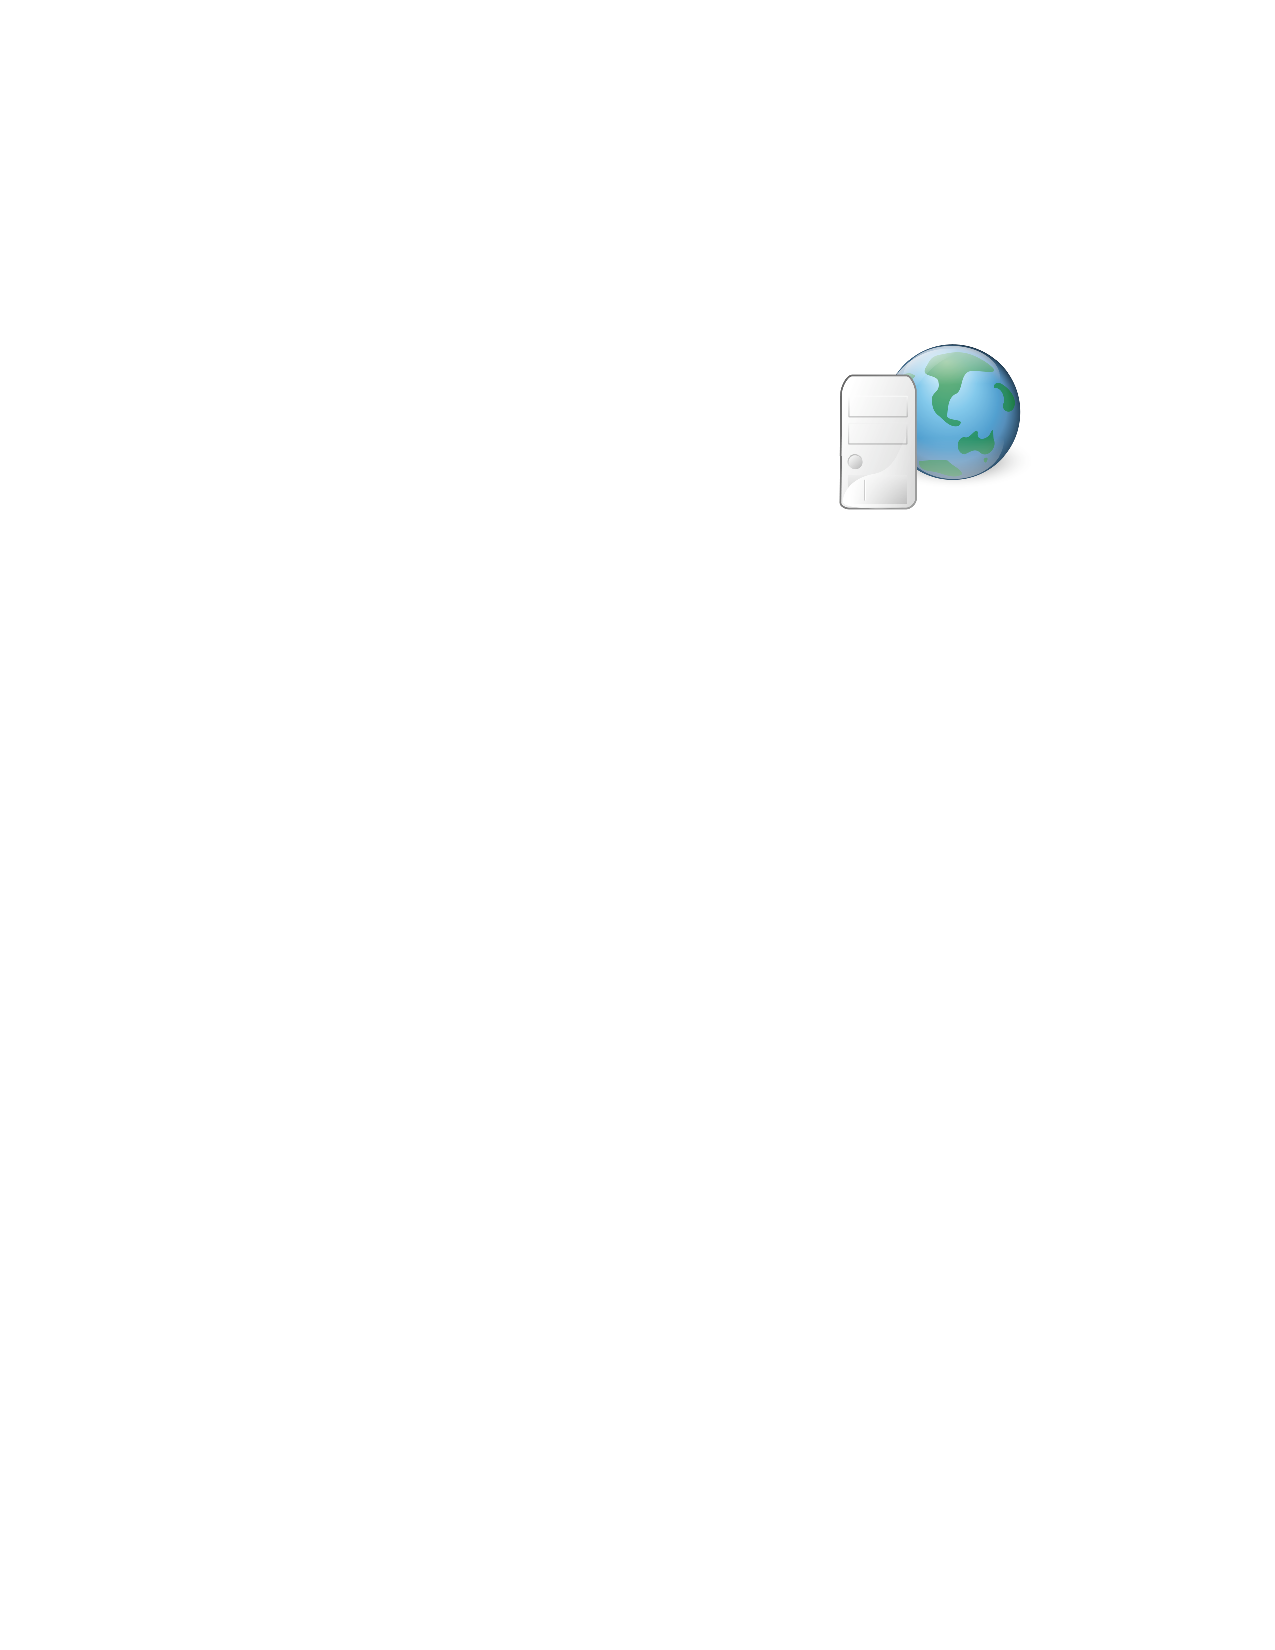
\includegraphics[width=1.75cm]{figures/webserver}}\\repository}};
	\node[block,green!50!black,very thick] (cvmfs) at (6cm,-9cm) {\parbox{3.5cm}{\centering{\scshape CernVM-FS +\\CernVM} public key}};
	
	\draw[->,gray,very thick] (release manager.west) -- node[gray,fill=white] {\parbox{2cm}{\centering
\includegraphics[width=1cm]{figures/fingerprint}\\ fingerprint}} (whitelist.north);
	\draw[->,gray,very thick] (release manager.east) -- node[gray,fill=white] {\parbox{2cm}{\centering
\includegraphics[width=1cm]{figures/sign-cert}\\ sign repository}} (web server.north);
	\draw[->,gray,very thick] (whitelist.east) -- node[white,fill] {\parbox{2cm}{\centering
\includegraphics[width=1cm]{figures/sign}\\ \textcolor{gray}{sign whitelist}}} ($(whitelist.east) + (8.75,0)$);
	
	\draw[->,very thick,blue!75,curve to,out=200,in=90] (web server.south west) to node[blue!75,fill=white] {\parbox{3cm}{\centering {\tikz \node[fill,draw,circle,inner sep=1pt]{\textcolor{white}1};}\\download\\signed catalog +\\signed whitelist}} (cvmfs.north);
	\node[blue!75,above left=of cvmfs,xshift=0.75cm,yshift=-0.75cm] {\parbox{3cm}{\centering {\tikz \node[fill,draw,circle,inner sep=1pt]{\textcolor{white}2};}\\verify whitelist +\\check fingerprint}};
	\draw[->,very thick,blue!75,curve to,out=270,in=45] (web server.south) to node[blue!75,below] {\parbox{2cm}{\centering {\tikz \node[fill,draw,circle,inner sep=1pt]{\textcolor{white}3};}\\download\\files}} (cvmfs.north east);
	\node[blue!75] at (6cm,-10.5cm) {\parbox{4cm}{\centering {\tikz \node[fill,draw,circle,inner sep=1pt]{\textcolor{white}4};}\\compare secure hash\\against catalog entry}};
\end{tikzpicture} 

%\end{document}

	\end{center}
	\caption{Trust chain with a signed repository.}
	\label{fig:security}
\end{figure}


%\section{Repository Layout}
%\label{sct:repository}

\section{Use of HTTP}
The particular way of using the \indexed{HTTP} protocol has significant impact on the performance and usability of \cvmfs.
If possible, \cvmfs\ tries to benefit from the HTTP/1.1 features keep-alive and cache-control.
Internally, \cvmfs\ uses the \product{libcurl} library~\cite{libcurl}.

The HTTP behaviour affects a system with cold caches only.
As soon as all necessary files are cached, there is only network traffic when a catalog TTL expires.
%Usually we'll see network traffic right after booting a \cernvm\ for the first time, after switching to another experiment environment, and after a new software version has been published.

The \cvmfs\ download manager runs as a separate thread that handles download requests asynchronously in parallel.
Concurrent download requests for the same URL are collapsed into a single request.

\subsection{DoS Protection}
A subtle denial of service attack (DoS) can occur when \cvmfs\ is successfully able to download a file but fails to store it in the local cache.
This situation escalates into a DoS when the application using \cvmfs\ remains in an endless loop and tries to open a file over and over again.
Such a situation is prevented by \cvmfs\ by re-trying with an exponential backoff.
%That prevents request storms to web servers from applications trying to open a file in an endless loop.
The backoff is triggered by consequtive filaures to cache a downloaded file within 10 seconds.

\subsection{Keep-Alive}
Although the HTTP protocol overhead is small in terms of data volume, in high latency networks we suffer from the bare number of requests: Each request-response cycle has a penalty of at least the network round trip time. 
Using plain HTTP/1.0, this results in at least $3\cdot\text{round trip time}$ additional running time per file download for TCP handshake, HTTP GET, and TCP connection finalisation.
By including the \texttt{Connection:~Keep-Alive} header into HTTP requests, we advise the HTTP server end to keep the underlying TCP connection opened.
This way, overhead ideally drops to just round trip time for a single HTTP GET.
The impact of the keep-alive feature is shown in Figure~\ref{fig:keepalive}.
\begin{figure}
	\begin{center}
		\resizebox{0.5\linewidth}{!}{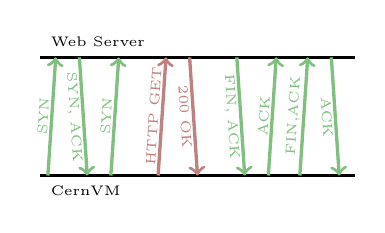
\begin{tikzpicture}
	[
		legend/.style={
			font=\tiny,
			outer sep=-2pt
		},
		legendframe/.style={
			font=\tiny
		},
		seq/.style={
			->, 
			very thick, 
			green!50!black!50	
		},
		http/.style={
			->, 
			very thick, 
			red!50!black!50	
		}
	]
	
	\draw[very thick]  (0,1.5) -- node[legendframe,above,anchor=south west] {Web Server} (0,1.5) -- (4,1.5);
	\draw[very thick]  (0,0) -- node[legendframe,below,anchor=north west] {CernVM} (0,0) -- (4,0);
	
	\draw[seq] (0.1,0) -- node[legend,sloped,above] {SYN} (0.2,1.5);
	\draw[seq] (0.5,1.5) -- node[legend,sloped,below] {SYN, ACK} (0.6,0);
	\draw[seq] (0.9,0) -- node[legend,sloped,above] {SYN} (1,1.5);
	
	\draw[http] (1.5,0) -- node[legend,sloped,above] {HTTP GET} (1.6,1.5);
	\draw[http] (1.9,1.5) -- node[legend,sloped,below] {200 OK} (2,0);
	
	\draw[seq] (2.5,1.5) -- node[legend,sloped,below] {FIN, ACK} (2.6,0);
	\draw[seq] (2.9,0) -- node[legend,sloped,above] {ACK} (3,1.5);
	\draw[seq] (3.3,0) -- node[legend,sloped,above] {FIN,ACK} (3.4,1.5);
	\draw[seq] (3.7,1.5) -- node[legend,sloped,below] {ACK} (3.8,0);
	
\end{tikzpicture}}
	\end{center}
	\caption{Impact of keep-alive header on multiple file downloads.}
	\label{fig:keepalive}
\end{figure}

This feature, of course, somewhat sabotages a server-side load-balancing.
However, exploiting the HTTP keep-alive feature does not affect scalability per se. 
The servers and proxies may safely close idle connections anytime, in particular if they run out of resources.
In practice, the maximum connection duration has to be set carefully for the HTTP deamon.

\subsection{Cache Control}
\label{sct:cachecontrol}
In a limited way, \cvmfs\ advises intermediate web caches how to handle its requests.
Therefor it uses the \texttt{Pragma:~no-cache} and the \texttt{Cache-Control:~no-cache} headers in certain cases.
These cache control headers apply to both, forward proxies as well as reverse proxies.
However, this is by no means a guarantee that intermediate proxies fetch a fresh original copy (though they should).

By including these headers, \cvmfs\ tries to not fetch outdated cache copies.
This has to be handled with care, of course, in order to not overload the repository source server.
Only in case \cvmfs\ downloads a corrupted file from a proxy server, it retries having the HTTP \texttt{no-cache} header set.
This way, the corrupted file gets replaced in the proxy server by a fresh copy from the backend.

\subsection{Identification Header}
\cvmfs\ sends a custom header (\lstinline{X-CMFS2}) to be identified by the web server.
If you have set the \cernvm\ GUID, this GUID is also transmitted.
%In \cernvm\ we use this header to rewrite URL's to the respective repository format for \cvmfs\ version 1 or \cvmfs\ version 2.

\section{Disk Cache}
\label{sct:mamangedcache}
Each running \cvmfs\ instance requires a local cache directory.
Data are downloaded into a temporary files.
Only at the very latest point they are renamed into their content-addressable SHA-1 names atomically by \texttt{rename()}.

The hard disk cache is managed, \ie \cvmfs\ maintains cache size restrictions and replaces files according to the \indexed{least recently used}\index{LRU|see{least recently used}} (LRU) strategy~\cite{lru06}.
In order to keep track of files sizes and relative file access times, \cvmfs\ sets up another \sqlite\ database in the cache directory, the \emph{cache catalog}.
The cache catalog contains a single table; its structure is shown in Table~\ref{tab:cachecatalog}.
\begin{table}
	\begin{center}
		\begin{tabular}{ll}
			\toprule
			\bf Field 							& \bf Type \\
			\midrule
			\bf SHA-1 							& String (hex notation) \\
			Size 								& Integer \\
			Access Sequence						& Integer \\
			Pinned								& Integer \\
			File type (chunk or file catalog)	& Integer\\
			\bottomrule
		\end{tabular}
	\end{center}
	\caption{Cache catalog table structure.}
	\label{tab:cachecatalog}
\end{table}

\cvmfs\ does not strictly enforce a the cache limit.
Instead \cvmfs\ works with two customizable soft limits, the \emph{cache quota} and the \emph{cache threshold}.
When exceeding the cache quota, files are deleted until the overall cache size is less than or equal to the cache threshold.
The cache threshold is currently hard-wired to half of the cache quota.
The cache quota is for data files as well as file catalogs.
Currently loaded catalogs are pinned in the cache, \ie they will not be deleted until unmount or until a new repository revision is applied.
On unmount, pinned file catalogs are updated with the highest sequence number.

The cache catalog can be re-constructed from scratch on mount.
Re-constructing the cache catalog is necessary when the managed cache is used for the first time and every time when ``unmanaged'' changes occurred to the cache directory, \eg when \cvmfs\ was terminated unexpectedly.
Re-construction has to be triggered manually.

In case of an exclusive cache, the cache manager runs as a separate thread of the \texttt{cvmfs2} process.
This thread gets notified by the Fuse module whenever a file is opened or inserted.  
Notification is done through a pipe.  
The shared cache uses the very same code, except that the thread becomes a separate process (see Figure~\ref{fig:sharedcache}).  
This cache manager process is not another binary but \texttt{cvmfs2} forks to itself with special arguments, indicating that it is supposed to run as a cache manager.  
The cache manager does not need to be started as a service.  
The first \cvmfs\ instance that uses a shared cache will automatically spawn the cache manager process.  
Subsequent \cvmfs\ instances will connect to the pipe of this cache manager.
Once the last \cvmfs\ instance that uses the shared cache is unmounted, the communication pipe is left without any writers and the cache manager automatically quits.

\begin{figure}
	\centering
	%\documentclass[a4paper, 11pt]{article}\usepackage{tikz,ifthen}\usetikzlibrary{circuits.logic.US,arrows,positioning,arrows,shapes,topaths,calc,fit,backgrounds,matrix,shadows,decorations.pathreplacing,decorations.text,trees}\usepackage[margin=2cm]{geometry}\begin{document}\sf

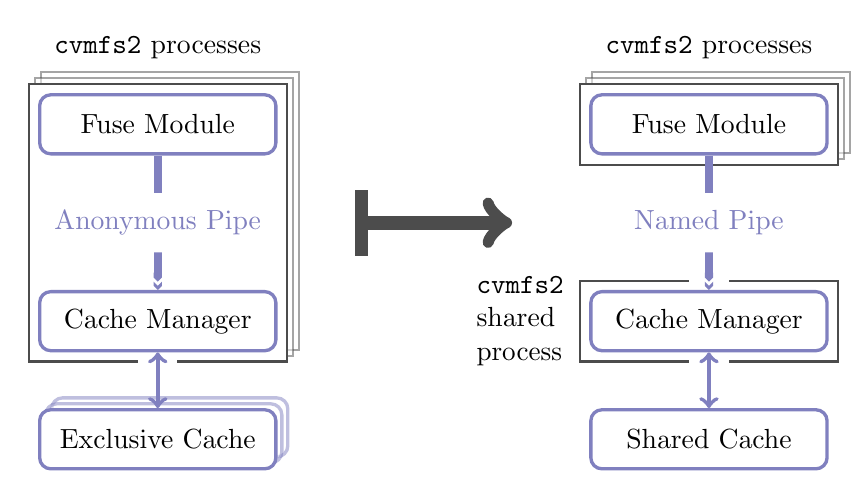
\begin{tikzpicture}
	[
		item/.style={
			rectangle,
			rounded corners,
			very thick,
			minimum width=3cm,
			minimum height=0.75cm,
			draw=blue!50!black!50,
		},
		process/.style={
			rectangle,
			thick,
			draw=black!70,
		}
	]

	\node[item] (threaded fuse) {Fuse Module};
	\node[item] (threaded mgr) at ($(threaded fuse)+(0, -2.5)$) {Cache Manager};
	
	\begin{pgfonlayer}{background}
		\node[process, fill=white, double copy shadow={opacity=0.5}, label={[label distance=5pt]above:{\texttt{cvmfs2} processes}}, fit=(threaded fuse)  (threaded mgr)] {};
	\end{pgfonlayer}
	
	\node[item, fill=white, double copy shadow={opacity=0.5}] (threaded cachedb) at ($(threaded mgr)+(0, -1.5)$) {Exclusive Cache};
	
	\draw[item, arrows=-fast cap, line width=3pt] (threaded fuse) -- node[blue!50!black!50, fill=white] {Anonymous Pipe}(threaded mgr); 
	\node[fill=white, anchor=north, minimum width=0.5cm] at (threaded mgr.south) {};
	\draw[item, <->, line width=1.5pt] (threaded mgr) -- (threaded cachedb); 
	
	%\draw[black!70, |-|, very thick] ($(threaded fuse.north west)-(0.75,-0.75)$) -- node[above, rotate=90] {$n$ times} ($(threaded cachedb.south west)-(0.75,0.1)$);
	
	
	
	\draw[black!70, |->, line width=5pt] (2.5,-1.25) -- (4.5,-1.25);
	
	
	\node[item] (shared fuse) at (7,0) {Fuse Module};
	\node[item] (shared mgr) at ($(shared fuse)+(0, -2.5)$) {Cache Manager};
	
	\begin{pgfonlayer}{background}
		\node[process, fill=white, double copy shadow={opacity=0.5}, label={[label distance=5pt]above:{\texttt{cvmfs2} processes}}, fit=(shared fuse)] {};
	\end{pgfonlayer}
	\node[process, label={[label distance=5pt]left:{\parbox{1cm}{\centering\texttt{cvmfs2}\\ shared\\ process}}}, fit=(shared mgr)] {};
	
	\node[fill=white, anchor=north, minimum width=0.5cm] at (shared mgr.south) {};
	\node[fill=white, anchor=south, minimum width=0.5cm] at (shared mgr.north) {};
	
	\draw[item, arrows=-fast cap, line width=3pt] (shared fuse) -- node[blue!50!black!50, fill=white] {Named Pipe} (shared mgr); 
	\node[item, fill=white] (shared cachedb) at ($(shared mgr)+(0, -1.5)$) {Shared Cache};
	\draw[item, <->, line width=1.5pt] (shared mgr) -- (shared cachedb); 
	
\end{tikzpicture}

%\end{document}

	\caption{The \cvmfs\ shared local hard disk cache.}
	\label{fig:sharedcache}
\end{figure}


\section{File System Traces}\index{traces}\index{file system traces|see{traces}}
\cvmfs\ has an optional file system operations tracer.
The tracer creates logs of usage, which can---for instance---be used as profiling information for pre-fetching.
The trace file is created in \indexed{CSV} format (see Figure~\ref{fig:traces}).
\begin{figure}
	\centering
	\begin{verbatim}
"1481074921.015","1","/root/i686-pc-linux-gnu/include/TQObject.h","OPEN"
"1481074931.030","1","/root/i686-pc-linux-gnu/include/KeySymbols.h","OPEN"
"1481074931.220","3","/root/i686-pc-linux-gnu/include/KeySymbols.h","READ (TRY)"
"1481074964.565","3","/root/i686-pc-linux-gnu/include/KeySymbols.h","READ 7407@0"
"1481074965.005","1","/root/i686-pc-linux-gnu/include/TRootCanvas.h","OPEN"
	\end{verbatim}
	\caption{Example snippet of a trace log. The first columns stores time stamps as number of microseconds starting from the Unix epoch. The second column stores the event type. Negative event types are reserved for \cvmfs\ internal events.}
	\label{fig:traces}
\end{figure}

The tracing runs in a separate thread and adapts the \emph{tread-safe trace buffer}, a technique used for multi-thread debugging~\cite[Chapter 8]{multicore06}.
Since traces are kept in a memory ring buffer\footnote{Usually, each trace record requires two atomic \texttt{fetch-and-add} operations.} and written to disk in blocks of thousands of lines, the performance overhead for tracing is low.

\section{NFS Maps}
In normal mode, \cvmfs\ issues inodes based on the row number of an entry in the file catalog.
When exported via NFS, this scheme can result in inconsistencies because \cvmfs\ does not control the cache lifetime of NFS clients.
A once issued inode can be asked for anytime later by a client. 
To be able to reply to such client queries even after reloading catalogs or remounts of \cvmfs, the \cvmfs\ \emph{NFS maps} implement a persistent store of the path names $\mapsto$ inode mappings.
Storing them on hard disk allows for control of the \cvmfs\ memory consumption (currently $\approx\SI{45}{\mega\byte}$ extra) and ensures consistency between remounts of \cvmfs. 
The performance penalty for doing so is small. 
\cvmfs\ uses Google's \leveldb\cite{leveldb}, a fast, local key value store. 
Reads and writes are only performed when meta-data are looked up in \sqlite, in which case the \sqlite\ query supposedly dominates the running time.

A drawback of the NFS maps is that there is no easy way to account for them by the cache quota. 
They sum up to some 150-200 Bytes per path name that has been accessed.
A recursive \texttt{find} on /cvmfs/atlas.cern.ch with 25 million entries, for instance, would add up \SI{5}{\giga\byte} in the cache directory.  
This is mitigated by the fact that the NFS mode will be only used on few servers that can be given large enough spare space on hard disk.

\section{Loader}

The \cvmfs\ \fuse\ module comprises a minimal \emph{loader} loader process (the \texttt{cvmfs2} binary) and a shared library containing the actual \fuse\ module (\texttt{libcvmfs\_fuse.so}).
This structure makes it possible to reload \cvmfs\ code and parameters without unmounting the file system.
Loader and library don't share any symbols except for two global structs \texttt{cvmfs\_exports} and \texttt{loader\_exports} used to call each others functions.  
The loader process opens the Fuse channel and implements stub \fuse\ callbacks that redirect all calls to the \cvmfs\ shared library.  
Hotpatch is implemented as unloading and reloading of the shared library, while the loader temporarily queues all file system calls in-between.  
Among file system calls, the Fuse module has to keep very little state.  
The kernel caches are drained out before reloading.  
Open file handles are just file descriptors that are held open by the process. 
Open directory listings are stored in a Google dense\_hash that is saved and restored. 

%\section{Pre-fetching}\index{pre-fetching}
%\label{sct:prefetching}

\section{File System Interface}
\label{sct:interface}

Since \cvmfs\ is a read-only file system, there are only few non-trivial call-back functions to implement.
These call-back functions provide the system interface.

\subsection{\tt mount}
On mount, the file catalog has to be loaded.
First, the file catalog \emph{manifest} \texttt{.cvmfspublished} is loaded.
The manifest is only accepted on successful validation of the signature.
In order to validate the signature, the certificate and the white-list are downloaded in addition if not found in cache.
If the download fails for whatever reason, \cvmfs\ tries to load a local file catalog copy.
As long as all requested files are in the disk cache as well, \cvmfs\ continues to operate even without network access (\emph{offline mode}).
If there is no local copy of the manifest or the downloaded manifest and the cache copy differ, \cvmfs\ downloads a fresh copy of the file catalog.

\subsection{{\tt getattr} and {\tt lookup}}
Requests for file attributes are entirely served from the mounted catalogs, \ie there is no network traffic involved.
This function is called as pre-requisite to other file system operations and therefore the most frequently called \fuse\ callback.
In order to minimize relatively expensive \sqlite\ queries, \cvmfs\ uses a hash table to store negative and positive query results.
The default size of \SI{16}{\mega\byte} for this memory cache is determined according to compilation benchmarks.

Additionally, the callback takes care of the catalog TTL.
If the TTL is expired, the catalog is re-mounted on the fly.
Note that a re-mount might possibly break running programs.
We rely on careful repository publishers that produce more or less immutable directory trees, \ie new repository versions just add files.

If a directory with a nested catalog is accessed for the first time, the respective catalog is mounted in addition to the already mounted catalogs.
Loading nested catalogs is transparent to the user.

\subsection{\tt readlink}
A symbolic link is served from the file catalog.
As a special extension, \cvmfs\ detects environment variables in symlink strings written as \texttt{\$(VARIABLE)}.
These variables are expanded by \cvmfs\ dynamically on access (in the context of the \texttt{cvmfs2} process).
This way, a single symlink can point to different locations depending on the environment.
This is helpful, for instance, to dynamically select software package versions residing in different directories.

\subsection{\tt readdir}
A directory listing is served by a query on the file catalog.
Although the ``parent''-column is indexed (\cf Table~\ref{tab:catalog}), this is a relatively slow function.
We expect directory listing to happen rather seldom.

\subsection{\tt open / read}
The \texttt{open()} call has to provide a file descriptor for a given path name.
In \cvmfs\ file requests are always served from the disk cache.
The \fuse\ file handle is a file descriptor valid in the context of the \cvmfs\ process.
It points into the disk cache directory.
Read requests are translated into the \texttt{pread()} system call.

\subsection{\tt getxattr}
\cvmfs\ uses extended attributes to display additional repository information.
There are two supported attributes:
\begin{description}
	\item[expires]
		Shows the remaining life time of the mounted root file catalog in minutes.
	\item[fqrn]
		Shows the fully qualified repository name of the mounted repository.
	\item[inode\_max]
		Shows the highest possible inode with the current set of loaded catalogs.		
	\item[hash]
		Shows the SHA-1 hash of a regular file as listed in the file catalog.
	\item[host]
		Shows the currently active HTTP server.
	\item[lhash]
		Shows the SHA-1 hash of a regular file as stored in the local cache, if available.
	\item[maxfd]
		Shows the maximum number of file descriptors available to file system clients.
	\item[nclg]
		Shows the number of currently loaded nested catalogs.
	\item[ndiropen]
		Shows the overall number of opened directories.
	\item[ndownload]
		Shows the overall number of downloaded files since mounting.
	\item[nioerr]
		Shows the total number of I/O errors encoutered since mounting.			
	\item[nopen]
		Shows the overall number of \texttt{open()} calls since mounting.
	\item[pid]
		Shows the process id of the \cvmfs\ \fuse\ process.		
	\item[proxy]
		Shows the currently active HTTP proxy.
	\item[rawlink]
	    Shows unresolved variant symbolic links; only accessible as root.
	\item[revision]
		Shows the file catalog revision of the mounted root catalog, an auto-increment counter increased on every repository publish.
	\item[root\_hash]
		Shows the SHA-1 hash of the root file catalog.
	\item[rx]
		Shows the overall amount of downloaded kilobytes.
	\item[speed]
		Shows the average download speed.
	\item[timeout]
		Shows the timeout for proxied connections in seconds.
	\item[timeout\_direct]
		Shows the timeout for direct connections in seconds.
	\item[rawlink]
		Shows the unresolved variant symlink.	
	\item[uptime]
		Shows the time passed since mounting in minutes.
	\item[usedfd]
		Shows the number of file descriptors currently issued to file system clients.		
	\item[version]
		Shows the version of the loaded \cvmfs\ binary.	
\end{description}

Extended attributes can be queried using the \texttt{attr} command.
For instance, \texttt{attr -g hash /cvmfs/atlas.cern.ch/ChangeLog} returns the SHA-1 key of the file at hand.
The extended attributes are used by the \texttt{cvmfs\_config stat} command in order to show a current overview of health and performance numbers.


\section{Repository Publishing}

Repositories are not immutable, every now and then they get updated. 
This might be installation of a new release or a patch for an existing release.  
But, of course, each time only a small portion of the repository is touched, say \SI{2}{\giga\byte} out of \SI{100}{\giga\byte}.
In order not to re-process an entire repository on every update, we create a read-write file system interface to a \cvmfs\ repository where all changes are written into a distinct scratch area.

\subsection{Read-write Interface using a Union File System}
Union file systems combine several directories into one virtual file system that provides the view of merging these directories.
These underlying directories are often called \emph{branches}.
Branches are ordered; in the case of operations on paths that exist in multiple branches, the branch selection is well-defined.
By stacking a read-write branch on top of a read-only branch, union file systems can provide the illusion of a read-write file system for a read-only file system.
All changes are in fact written to the read-write branch.

Preserving POSIX semantics in union file systems is non-trivial; the first fully functional implementation has been presented by Wright et al.~\cite{unionfs04}.
By now, union file systems are well established for ``Live CD'' builders, which use a RAM disk overlay on top of the read-only system partition in order to provide the illusion of a fully read-writable system.
\cvmfs\ uses the AUFS union file system.
Another union file system with similar semantics can be plugged in if necessary.

Union file systems can be used to track changes on CernVM-FS repositories (Figure~\ref{fig:overlay}).
In this case, the read-only file system interface of CernVM-FS is used in conjunction with a writable scratch area for changes.

\begin{figure}
	\begin{center}
		\resizebox{0.5\textwidth}{!}{%\documentclass[a4paper, 11pt]{article}\usepackage{tikz,ifthen}\usetikzlibrary{arrows,positioning,shapes,topaths,calc,fit,backgrounds,matrix,shadows}\begin{document}

\newsavebox{\tikzfilesystemovl}
\savebox{\tikzfilesystemovl}{
\begin{tikzpicture}
	[
		dirent/.style={
			circle,
			draw=green!50!black!50,
			fill=green!50!black!50,
			scale=0.35pt
		}
	]
	\node[dirent] (root) at (0,1.6) {};
	\node[dirent,red!50!black!50,fill=red!50!black!50] (d1) at (0.4, 1.2) {};
	\node[dirent] (d2) at (0.4, 0.8) {};
	\node[dirent,red!50!black!50,fill=red!50!black!50] (d21) at (0.8, 0.4) {};
	\node[dirent] (d22) at (0.8, 0) {};
	
	\draw (root) -- (0,1.2) -- (d1);
	\draw (0,1.2) -- (0,0.8) -- (d2) -- (0.4, 0.4) -- (d21);
	\draw (0.4,0.4) -- (0.4,0) -- (d22);
	\draw (0,0.8) -- (0,0);		
	
	\node at (-0.2,0.1) {
\includegraphics[height=1cm]{figures/folder}};
\end{tikzpicture}
}

\begin{tikzpicture}
	\tikzstyle{every node}=[font=\large]
	\colorlet{colrepo}{blue!50}
	\colorlet{colscratch}{red!40}
	\colorlet{colunion}{blue!50!black}

	\node[fill=colrepo, semitransparent, trapezium, trapezium left angle=30, trapezium right angle=-30, minimum width=9.5cm] (repository) {};
	\node[blue, anchor=south, xshift=0.5cm] at (repository.bottom side) {CernVM-FS Read-Only};
	
	\node[fill=colscratch, semitransparent, drop shadow, trapezium, trapezium left angle=30, trapezium right angle=-30, minimum width=9.25cm] (scratch) at ($(repository)+(0.75, 0.75)$) {};
	\node[red!80!black, anchor=south, xshift=0.5cm] at (scratch.bottom side) {Read/Write Scratch Area};
	
	\draw[colunion, ->, line width=1ex, rounded corners] (4,-0.5) -- node[fill=white] {\parbox{4.5cm}{\centering AUFS\\(Union File System)}} ++(0,-2) -- ++(-3.75,0);
	
	\node[draw, rectangle, very thick, colunion, rounded corners, minimum width=4.75cm, minimum height=2.75cm] at (-2.5, -3) {};
	\node[label={[colunion, label distance=-0.5cm]left:\parbox{2.5cm}{Read/Write\\ Interface}}] at (-1.25, -3) {\usebox{\tikzfilesystemovl}};
\end{tikzpicture}

%\end{document}}
	\end{center}
	\label{fig:overlay}
	\caption{A union file system combines a CernVM-FS read-only mount point and a writable scratch area.  
		It provides the illusion of a writable CernVM-FS mount point, tracking changes on the scratch area.}
\end{figure}

Based on the read-write interface to CernVM-FS, we create a feed-back loop that represents the addition of new software releases to a CernVM-FS repository.
A repository in base revision $r$ is mounted in read-write mode on the publisher's end.
Changes are written to the scratch area and, once published, are re-mounted as repository revision $r+1$.
In this way, CernVM-FS provides snapshots. 
In case of errors, one can safely resume from a previously committed revision.


%\chapter{Sample Infrastructure Setup}

\appendix
%\chapter{\deprecated{A Release Manager Machine for \zep}}
\label{apx:releasemgr}
At \cern\ we host repositories using OpenSolaris/ZFS, Apache, and Squid servers running on a VMware vSphere virtualized infrastructure.
However, for small VOs similar functionality can be achieved with a single standard SLC5 machine.

So, let's assume you are software manager for the ambitious and imaginary \zep\ experiment driven by the famous and imaginary Aviation Research Institute.
Recently you decided to distribute your software packages with \cvmfs\ and you are in charge of maintaining the releases.
So you acquired an SLC5 machine and an additional harddisk that is supposed to store the repository.
The machine is available from the outside as \texttt{zeppelin-webfs.aviation-research.org}.

\section{Roadmap}
The release manager machine will have three purposes:
\begin{enumerate}
	\item Serve as a template machine where software releases are installed and tested
	\item Store snapshots of the software releases
	\item Publish releases via HTTP
\end{enumerate}
Software releases will be installed in \texttt{/opt/zeppelin}, which is supposed to be a self-contained software directory.
We use the logical volume manger (LVM) in order to create snapshots of different releases.
These snapshots are mounted read-only in \texttt{/srv/www/webfs} and served to the outside by Apache under \url{http://zeppelin-webfs.aviation-research.org/opt/zeppelin}.
This way you are able to install and test new software releases while always serving a consistent repository.

\section{Initial Setup}
We start by installing the necessary software for the rest of the installation procedure.
Make sure, the following SLC5 packages are installed:
\begin{lstlisting}[language=bash]
yum install autoconf automake gcc gcc-c++ pcre-devel curl-devel \
            openssl-devel fuse fuse-devel screen httpd
\end{lstlisting}
Additionally we require \texttt{inotify-tools}.
The tarball can be downloaded from \url{http://inotify-tools.sourceforge.net}.
After untaring, the installation is a straight forward \lstinline{./configure; make; make install}.

We now have the necessary requirements to build and install \cvmfs.
Download the latest tarball from \url{https://cernvm.cern.ch/project/trac/cernvm/downloads} (cf.~Section \ref{sct:start}).
Note that we need to work with the tarball since we require the server part and additional scripts not shipped with the RPM.
After untaring we build and install by
\begin{lstlisting}[language=bash]
./configure --enable-sqlite3-builtin --enable-libcurl-builtin
make
make install
\end{lstlisting}

It's now time to prepare the repository harddisk, which we assume to be located at \texttt{/dev/sdb}.
We start the interactive utility \lstinline{/usr/sbin/parted /dev/sdb} to initialize the disk.
We use the \lstinline{print} command to make sure we see the empty partition table of the correct harddisk.
Also, remember the size of the harddisk as shown by \lstinline{print}.
We create an ms-dos partition table by \lstinline{mklabel} and a primary partition spanning the entire size with \lstinline{mkpart}.
We check again with \lstinline{print} and leave the utility with \lstinline{quit}.
Now there should be \texttt{/dev/sdb} and \texttt{/dev/sdb1}

The next step is to setup LVM in the newly created partition.
At this point, we have to estimate a maximum size of the software repository.
In order to make sure that snapshots never become unusable, each snapshot has to have at least the size of the working repository.
So the size of the harddisk should be large enough to store the working repository and a couple of snapshots.
For this tutorial, let's assume a 200\,GB harddisk and an upper bound of 20\,GB for the repository.
The following commands set up the repository volume:
\begin{lstlisting}[language=bash]
/usr/sbin/pvcreate /dev/sdb1
/usr/sbin/vgcreate vg-zeppelin /dev/sdb1
/usr/sbin/lvcreate -L 20G -n lv-zeppelin vg-zeppelin
/sbin/mkfs.ext3 /dev/vg-zeppelin/lv-zeppelin
\end{lstlisting}
The volume ist supposed to be mounted at \texttt{/srv/cvmfs/zeppelin}.
We create the necessary directory hieves by:
\begin{lstlisting}[language=bash]
mkdir -p /srv/cvmfs/zeppelin # working repository
mkdir -p /srv/www/webfs/zeppelin # Apache document root
mkdir -p /opt/zeppelin # Install and test your software here

# Create repository directory structure
mount  /dev/vg-zeppelin/lv-zeppelin /srv/cvmfs/zeppelin
mkdir -p /srv/cvmfs/zeppelin/pub/catalogs /srv/cvmfs/zeppelin/pub/data \
         /srv/cvmfs/zeppelin/ctrl /srv/cvmfs/zeppelin/shadow
umount /srv/cvmfs/zeppelin
\end{lstlisting}
To mount the volume persistently we edit \texttt{/etc/fstab} and add the lines
\begin{lstlisting}[language=bash]
/dev/vg-zeppelin/lv-zeppelin  /srv/cvmfs/zeppelin  ext3  defaults       0 0
/srv/cvmfs/zeppelin/shadow    /opt/zeppelin        bind  defaults,bind  0 0
\end{lstlisting}
We test the changes with \lstinline{mount -a; mount}.

As last step, we create a user to install and test software.
This user becomes owner of the repository, \ie we run
\begin{lstlisting}[language=bash]
useradd zeppelin
chown -R zeppelin:zeppelin /srv/cvmfs/zeppelin
\end{lstlisting}

\section{Maintaining the Repository}
Your software will be installed in \texttt{/opt/zeppelin}.
This directory has to be under surveillance of \texttt{cvmfs\_journald}.
This utility records all the changes to the \texttt{/opt/zeppelin} directory in order to synchronize it with the \cvmfs\ repository (cf.~Section~\ref{sct:createrepo}).
You can use the \texttt{initd} script in the \texttt{add-ons} directory of the \cvmfs\ tarball.
The important command to startup the utility is
\begin{lstlisting}[language=bash]
screen -dmS cvmfs_journald sudo -u zeppelin sh -c \
 "LD_LIBRARY_PATH=/usr/local/lib:$LD_LIBRARY_PATH /usr/local/bin/cvmfs_journald\
 -w /opt/zeppelin -r /srv/cvmfs/zeppelin/pub -e /srv/cvmfs/zeppelin/inotify_events\
 -l /src/cvmfs/zeppelin/ctrl/log -s /srv/cvmfs/zeppelin/ctrl/in_sync\
 -o /srv/cvmfs/zeppelin/ctrl/ready -a  /srv/cvmfs/zeppelin/ctrl/auth\
 | tee /srv/cvmfs/zeppelin/ctrl/stdout"
\end{lstlisting}
Always make sure that \texttt{cvmfs\_journald} is running before making changes to the repository.
As root you can check with \lstinline{screen -x cvmfs_journald}.

Now switch to user zeppelin by \lstinline{su zeppelin} and install and test your installation.
For now we just create a single file with \lstinline{echo "Hello, CVMFS" > /opt/zeppelin/README}.
For publishing it, we switch back to root, create and LVM snapshot and mount it under \texttt{/srv/www/webfs/zeppelin}.
In the \texttt{add-ons} directory of the \cvmfs\ tarball you'll find the \texttt{cvmfs-publish} shell script that wraps up all the necessary steps.
Listing~\ref{lst:publish} shows the essential commands from that script.
\begin{lstlisting}[caption=Excerpt from \texttt{cvmfs-publish} utility,label=lst:publish,language=bash]
REPOSITORY=$1
COMMAND=$2

switch_snapshot ()
{
  snapshot=$1
  fstabline="/dev/vg-$REPOSITORY/$snapshot /srv/www/webfs/$REPOSITORY \
             ext3 defaults,ro 0 0 #CVMFS_AUTOPUBLISH"
  grep -v CVMFS_AUTOPUBLISH /etc/fstab > /etc/fstab.2
  echo $fstabline >> /etc/fstab.2
  mv /etc/fstab.2 /etc/fstab
  umount /srv/www/webfs/$REPOSITORY 2>/dev/null
  mount -a
}

case $COMMAND in
  list)
    snapshots=`ls /dev/vg-$REPOSITORY/ 2>/dev/null`
    for s in $snapshots
    do
      echo $s
    done    
  ;;
  publish)
    origin="/dev/vg-$REPOSITORY/lv-$REPOSITORY"
    size=`lvs --noheadings -o lv_size --units K $origin`

    touch /opt/$REPOSITORY/.cvmfscatalog 
    sleep 2
    while [ ! -f /srv/cvmfs/$REPOSITORY/ctrl/in_sync ]; do
      sleep 2
    done
    
    timestamp=`date "+%Y%m%d%H%M%S"`
    snapshot=lv-$REPOSITORY-$timestamp
    /usr/sbin/lvcreate -s -L $size -p r -n $snapshot $origin
    
    switch_snapshot $snapshot
  ;;
  switch)
    snapshot=$3
    switch_snapshot $snapshot
  ;;
  remove)
    snapshot=$3
    /usr/sbin/lvremove /dev/vg-$REPOSITORY/$snapshot
  ;;
esac
\end{lstlisting}
So we run \lstinline{cvmfs-publish zeppelin publish} and check with \lstinline{cvmfs-publish zeppelin list}.

\section{Apache Configuration}
We are almost done.
The last step is to make Apache publish \texttt{/srv/www/webfs/zeppelin}.
To do so, we first add the apache user to the zeppelin group by \lstinline{usermod -a -G zeppelin apache}.
Then we drop an Apache configure file in \texttt{/etc/httpd/conf.d/webfs.conf}.
This configuration will create a virtual directory \url{http://zeppelin-webfs.aviation-research.org/opt} without touching the rest of your Apache configuration.
You can find the \texttt{initd} script in the \texttt{add-ons} directory of the \cvmfs\ tarball.
Listing~\ref{lst:apache} shows the essential options from that configuration file.
\begin{lstlisting}[caption=Excerpt from \texttt{webfs.conf} Apache configuration,label= lst:apache,language=bash]
RewriteEngine on

#  - /opt/<experiment> is forced to be lower case 
RewriteMap toLower int:tolower

# Lowering the case for repository names
RewriteRule ^/opt/([A-Za-z0-9\-\.]+)/(.*)$ /opt/${toLower:$1}/pub/catalogs/$2 [PT] 

# Translation URL to real pathname
Alias /opt /srv/www/webfs

# Close access to non-pub directories
<DirectoryMatch /srv/www/webfs/[A-Za-z0-9\-\.]+/(shadow|ctrl)>
    Order allow,deny
    Deny from all
</DirectoryMatch>

<Directory "/srv/www/webfs">
    Options Indexes -MultiViews FollowSymLinks
    AllowOverride All
    Order allow,deny
    Allow from all

    IndexOptions +SuppressDescription +FoldersFirst +VersionSort +SuppressIcon

    EnableMMAP Off
    EnableSendFile Off

    AddType application/x-compress-cvmfs .cvmfschecksum

    FileETag INode MTime Size 
    ExpiresActive On
    ExpiresDefault "access plus 15 minutes"
    ExpiresByType text/html "access plus 5 minutes" 
    ExpiresByType application/x-compress-cvmfs "access" 
</Directory>
\end{lstlisting}

At this point, we have to deal with some of the security measures in SLC5.
In particular, SELinux and iptables will shield you from all the dangers in the world.
Apart from that, they will also shield your users from accessing the repository.
So, as a first step, we tell SELinux that the repository is really supposed to be served by Apache (note that we have to publish again afterwards)
\begin{lstlisting}
chcon -h -R -t httpd_sys_content_t /srv/cvmfs/zeppelin
cvmfs-publish zeppelin publish
\end{lstlisting}
Secondly, in order to let other machines talk to your release manager machine, you have to open TCP port 80 in iptables.
There is a configuration utility to do that without editing the iptables configuration files.
Run \lstinline{system-config-securitylevel} (text based), go to ``customize'' and open WWW for incoming traffic.

\section{Test the Release Manager Machine}
The first step is to open a web browser and look if you can browse through \url{http://zeppelin-webfs.aviation-research.org/opt/zeppelin}.
You should be able to jump to the \texttt{data} directory and in the subdirectories within \texttt{data}.
In case there are any errors, \texttt{/var/log/httpd/access\_log} and \texttt{/var/log/httpd/error\_log} might contain useful information.
For SELinux, looking into \texttt{/var/log/audit/audit.log} might be helpful as well.

To test with the \cvmfs\ client part, we run the following commands:
\begin{lstlisting}
modprobe fuse
mkdir -p /var/cache/cvmfs2/default /mnt/cvmfs
cvmfs2 /mnt/cvmfs http://localhost/opt/zeppelin
cat /mnt/cvmfs/README
umount /mnt/cvmfs
\end{lstlisting}
In case of success, we have just observed a \texttt{Hello, CVMFS}.
\chapter{Available RPMs}
\label{apx:rpms}

The \cvmfs\ software is available in form of several RPM packages:
\begin{description}
	\item[cvmfs-release] Adds the \cvmfs\ yum repository.
	\item[cvmfs-keys] Contains the public key for signature verification of repositories in the cern.ch domain.
	\item[cvmfs] Contains the Fuse module and additional client tools.  It has dependencies to cvmfs-keys, fuse, and autofs.
	\item[cvmfs-devel] Contains the \texttt{libcvmfs.a} static library and the \texttt{libcvmfs.h} header file for use of \cvmfs\ with Parrot\cite{parrot05}.
	\item[cvmfs-init-scripts] Contains special settings for some of the repositories.
		For instance, the ATLAS nightly builds are provided by a URL other than the other repositories in cern.ch.
		Depends on cvmfs.
	\item[cvmfs-auto-setup] Only available through yum. 
		This is a wrapper for \texttt{cvmfs\_config setup}. 
		This is supposed to provide automatic configuration for the ATLAS Tier3s.
		Depends on cvmfs.
	\item[cvmfs-server] Contains the \cvmfs\ server tool kit for maintaining Stratum~0 and Stratum~1 servers.
		Depends on cvmfs-keys and httpd.
	\item[kernel-$\cdots$-.aufs21] Scientific Linux 6 kernel with aufs.
		Required for SL6 based Stratum~0 servers.
	\item[cvmfs-unittests] Contains the \texttt{cvmfs\_unittests} binary.  Only required for testing.
\end{description}

\chapter{\cvmfs\ Parameters}
\label{apx:parameters}

\section{Client parameters}
Parameters recognized in configuration files under /etc/cvmfs:
 

\section{Server parameters}

\chapter{\cvmfs\ Server Infrastructure}
\label{apx:serverinfrastructure}

This is trying to be a full documentation of a \cvmfs\ server setup including the infrastructure necessary for an individual repository.
It is highly recommended to first consult Section~\ref{sct:repoanatomy} for a more general overview of the involved directory structure.

\section{Prerequisites}
A \cvmfs\ server installation depends on some environment setup and tools to be in place:
\begin{itemize}
\item \aufs\ support in the kernel (see Section~\ref{sct:customkernelinstall})
\item Backend storage location available through HTTP
\item \textbf{cvmfs} and \textbf{cvmfs-server} packages installed
\end{itemize}

\section{Local Backend Storage Infrastructure}
\cvmfs\ stores the entire repository content (file content and meta-data catalogs) into a content addressable storage (CAS).
This storage can either be a file system at \texttt{/srv/cvmfs} or an S3 compatible key-value storage system (see Section~\ref{sct:s3storagesetup} for details).
In the former case the contents of \texttt{/srv/cvmfs} are as follows:

\LTXtable{\textwidth}{figures/tablocalstorageanatomy.tex}
\pagebreak

\section{Server Spool Area of a Repository (Stratum0)}
The spool area of a repository contains transaction infrastructure and scratch area of a Stratum0 or specifically a release manager machine installation.
It is always located inside \texttt{/var/spool/cvmfs} with directories for individual repositories.
Note that the data volume of the spool area can grow very large for massive repository updates since it contains the writable AUFS branch and a \cvmfs\ client cache directory.

\LTXtable{\textwidth}{figures/tabrepospoolanatomy.tex}
\pagebreak

\section{Repository Configuration Directory}
The authoritative configuration of a \cvmfs\ repository is located in \texttt{/etc/cvmfs/repositories.d} and should only be writable by the administrator.
Furthermore the repository's keychain is located in \texttt{/etc/cvmfs/keys} and follows the naming convention \texttt{<fqrn>.crt} for the certificate, \texttt{<fqrn>.key} for the repository's private key and \texttt{<fqrn>.pub} for the public key.
All of those files can be symlinked somewhere else if necessary.

\LTXtable{\textwidth}{figures/tabrepoconfiganatomy.tex}
\pagebreak


\pagestyle{plain}
\bibliographystyle{alpha}
\bibliography{references}

%\printindex

\end{document}
